\documentclass[letterpaper]{article}
\usepackage{authblk}

\usepackage[footnotes,definitionLists,hashEnumerators,smartEllipses,hybrid]{markdown}
\usepackage{adjustbox}
\usepackage{natbib,alifeconf}  %% The order is important
\usepackage[table,xcdraw]{xcolor}
\usepackage{subcaption}
\usepackage{longtable}
\usepackage{listings}
\usepackage{amsmath}
\usepackage{hyperref,cleveref}
\usepackage[moderate]{savetrees}
\usepackage[parfill]{parskip}
\usepackage{rotating}
\usepackage{tabularx}
\usepackage{rotating}
\usepackage{pdflscape,lipsum}
\usepackage{eso-pic,zref-user}
% \newcounter{cntsideways}
\usepackage{fancyheadings}
\usepackage{tikz}
\usetikzlibrary{calc}
\usepackage{orcidlink}

\usepackage{floatpag}
\floatpagestyle{plain}
\fancypagestyle{mylandscape}{%
  \fancyhf{}% Clear header/footer
  \fancyfoot{% Footer
  % adapted from https://tex.stackexchange.com/a/9086
  \tikz[remember picture,overlay]
        \node[outer sep=0.5in,above,rotate=90] at (current page.east) {\thepage};}  \renewcommand{\headrulewidth}{0pt}% No header rule
  \renewcommand{\footrulewidth}{0pt}% No footer rule
}

% adapted from https://tex.stackexchange.com/a/472608
\usepackage{eso-pic,zref-user}
\newcounter{cntsideways}
\makeatletter
\AddToShipoutPictureBG{%
  \PLS@RemoveRotate
}
\AddToShipoutPictureBG{%
 \ifnum\zref@extractdefault{rotate\number\value{page}}{page}{0}=0
  \PLS@RemoveRotate
 \else
  \PLS@AddRotate{90}%
 \fi}

\newcommand\rotatesidewayslabel{\stepcounter{cntsideways}%
 \zlabel{tmp\thecntsideways}\zlabel{rotate\zref@extractdefault{tmp\thecntsideways}{page}{0}}}

\let\originalsidewaysfigure\sidewaysfigure
\let\endoriginalsidewaysfigure\endsidewaysfigure
\renewenvironment{sidewaysfigure}{%
  \begin{originalsidewaysfigure}%
  \thisfloatpagestyle{mylandscape}%
  \rotatesidewayslabel%
}{%
  \end{originalsidewaysfigure}%
}

% \renewenvironment{sidewaysfigure*}{%
%   \begin{originalsidewaysfigure}%
%   \thisfloatpagestyle{mylandscape}%
%   \rotatesidewayslabel%
% }{%
%   \end{originalsidewaysfigure}%
% }

\let\originalsidewaystable\sidewaystable
\let\endoriginalsidewaystable\endsidewaystable
\renewenvironment{sidewaystable}{%
  \begin{originalsidewaystable}%
  \thisfloatpagestyle{mylandscape}%
  \rotatesidewayslabel%
}{%
  \end{originalsidewaystable}%
}
\renewenvironment{sidewaystable*}{%
  \begin{originalsidewaystable}%
  \thisfloatpagestyle{mylandscape}%
  \rotatesidewayslabel%
}{%
  \end{originalsidewaystable}%
}

\let\originallandscape\landscape
\let\endoriginallandscape\endlandscape
\renewenvironment{landscape}{%
  \begin{originallandscape}%
  \thispagestyle{mylandscape}%
  \rotatesidewayslabel%
}{%
  \end{originallandscape}%
}

\makeatother

%%% Renew command for full page figures:
\renewcommand{\topfraction}{1.0}

% Blank page (if needed)
\newcommand\blankpage{%
    \null
    \thispagestyle{empty}%
    \addtocounter{page}{-1}%
    \newpage}


% pragma once, adapted from https://tex.stackexchange.com/a/195173
\makeatletter
\let\pragma@iinput=\@iinput
\def\@iinput#1{\xdef\@pragmafile{#1}\pragma@iinput{#1}}
\def\@pragmafile{default}
\def\pragmaonce{%
   \csname pragma@\@pragmafile\endcsname
   \global\expandafter\let \csname pragma@\@pragmafile\endcsname = \endinput
}
\makeatother

\ifdefined\mydraft
\mydraft
\fi

% \setcounter{tocdepth}{4}
% \setcounter{secnumdepth}{4}

% *****************
%  Requirements:
% *****************
%
% - All pages sized consistently at 8.5 x 11 inches (US letter size).
% - PDF length <= 8 pages for full papers, <=2 pages for extended
%    abstracts (not including citations).
% - Abstract length <= 250 words.
% - No visible crop marks.
% - Images at no greater than 300 dpi, scaled at 100%.
% - Embedded open type fonts only.
% - All layers flattened.
% - No attachments.
% - All desired links active in the files.

% Note that the PDF file must not exceed 5 MB if it is to be indexed
% by Google Scholar. Additional information about Google Scholar
% can be found here:
% http://www.google.com/intl/en/scholar/inclusion.html.


% If your system does not generate letter format documents by default,
% you can use the following workflow:
% latex example
% bibtex example
% latex example ; latex example
% dvips -o example.ps -t letterSize example.dvi
% ps2pdf example.ps example.pdf


% For pdflatex users:
% The alifeconf style file loads the "graphicx" package, and
% this may lead some users of pdflatex to experience problems.
% These can be fixed by editing the alifeconf.sty file to specify:
% \usepackage[pdftex]{graphicx}
%   instead of
% \usepackage{graphicx}.
% The PDF output generated by pdflatex should match the required
% specifications and obviously the dvips and ps2pdf steps become
% unnecessary.


% Note:  Some laser printers have a serious problem printing TeX
% output. The use of ps type I fonts should avoid this problem.

\begin{document}

% Case Study Examining Novelty, Complexity, Adaptation, and Fraternal Evolutionary Transition in Individuality

\title{
    Loose Coupling in the Evolution of Novelty, Complexity, and Adaptation under Biotic Selection
    % along a lineage?
    %: (something about digital evolution?)
}
% A Case Study Examining Novelty, Complexity, and Adaptation during Evolutionary Transitions in Individuality
% A Case Study of Life Histories during Evolutionary Transitions in Individuality
% A Case Study Exploring Novelty, Complexity, and Adaptation during Evolutionary Transitions in Individuality <-- final choice
\author{
    Matthew Andres Moreno\orcidlink{0000-0003-4726-4479}$^{1,2,3,4,\dagger}$,\ %
    Santiago Rodriguez Papa\orcidlink{0000-0002-6028-2105}$^{5,7}$,\ %
    Charles Ofria\orcidlink{0000-0003-2924-1732}$^{5,6,7}$ \\
    \mbox{}\\
    $^1$Department of Ecology and Evolutionary Biology
    $^2$Center for the Study of Complex Systems \\
    $^3$Michigan Institute for Data and AI in Society
    $^4$University of Michigan, Ann Arbor, USA \\
    $^5$Department of Computer Science and Engineering
    $^6$Program in Ecology, Evolution, and Behavior \\
    $^7$Michigan State University, East Lansing, USA \\
    $^\dagger$\texttt{morenoma@umich.edu}
}

\maketitle

% For several authors from the same institution use the same number to
% refer to one address.
%
% If the names do not fit well on one line use
%         Author 1, Author 2 ... \\ {\Large\bf Author n} ...\\ ...
%
% If the title and author information do not fit in the area
% allocated, place \setlength\titlebox{<new height>} after the
% \documentclass line where <new height> is 2.25in

% redefine subsubsection so that there's a newline after every header
% taken from https://tex.stackexchange.com/a/60438
% \makeatletter
% \def\subsubsection{\@startsection{subsubsection}{3}%
%   \z@{.5\linespacing\@plus.7\linespacing}{.1\linespacing}%
%   {\normalfont\itshape}}
% \makeatother


\begin{abstract}
Biotic selection, the emergent interplay between evolutionary processes and environmental effects driven by evolved traits, is broadly considered essential to the diversity and sophistication characteristic of biological life.
For this reason, substantial interest exists as to how changes in novelty, complexity, and adaptation unfold along lineages under selection driven by freeform, localized biotic interactions.
%  multidimensional, localized
% freeform, arbitrary, open to _______?
% it remains unclear to what
In particular, fundamental questions include whether novelty, complexity, and adaptation arise gradually versus episodically, and the extent to which they are coupled.
% extent to which these phenomena are coupled, and whether they spike in discrete events or are more gradual.
% In conjunction with , Experimental approaches to classical work concerning hypothetical plausibility of isolated scenarios, attempting to reproduce ETIs under controlled conditions tests the sufficiency of an integrated model to account for the origins of biological structure and complexity in concrete instances.
To explore these topics, we examine a detailed evolutionary history encompassing two sequential morphological novelties, drawn from a digital multicell model incorporating extensive biotic interactions.
% an \textit{in silico} model system competition for space and resources among multicell groups.
% open to arbitrary biotic interactions among independent replicator cells capable of arbitrary behaviors.
Using knockout experiments and competition trials, we trace quantitative measures of fitness, phenotypic complexity, and genetic complexity across a series of 100 intermediate snapshots captured across evolutionary time.
%  through knockout experiments and fitness changes through competition trials, we plot out a detailed evolutionary context timeline surrounding these novelties across a series of 100 snapshot specimens. % captured across evolutionary time.
% We two phenotypic novelties in  arise — we see first cell groups adopt asymmetrical patterning; subsequently, we see these groups add a later secondary coordinated burst of outwards growth.
We find the establishment of an asymmetrical cigar patterning among multicells to be accompanied by moderate increases in both genetic complexity and fitness, as well as a substantial spike in phenotypic complexity.
However, later introduction of coordinated bursts in outward growth is accompanied by none of these effects.
% In a subsequent episode, a genome expansion drove strong fitness increase, but no notable changes in morphology or any complexity measures.
% Furthermore, strongest fitness effects are associated with no changes in genetic or phenotypic complexity --- although a notable later adaptive increase in genome size is observed.
Confirming the presence of biotic selection, we find some competition outcomes to reverse based on background presence of other evolved lineages.
Surprisingly, though, in one case we observe this effect associated with a sharp decrease in complexity and a loss of multicell patterning.
% Furthermore, late in evolutionary history, we see a sudden increase in genome size with strong fitness advantage but no apparent changes in complexity or life history.
% In several sampled, apparent "dead-end" lineages, we see apparent reversions with and loss of cooperative traits.
% Our a concrete
Finally, in partial contrast to adaptationist framings of biological complexity, we do not find increases in genetic complexity to be directly associated with fitness gains.
Instead, increases in genetic complexity are significantly associated with future fitness gains, possibly indicative of a potentiating relationship.
% with complexity increase not significantly associated with fitness benefit, but
On the other hand, our observation that complexity measures sometimes --- albeit inconsistently --- spike coincident with morphological novelty partially supports adaptationist framings of complexity.
% Providing a detailed, concrete glimpse into the evolution of complexity, novelty, and adaptation under a regime influenced by biotic selection,
% and provide a foundation for future work in tandem with new avenues of experimental evolution in \textit{in vivo},
% foundation for future work with replay experiments and multistrain tests across independent evolutionary trajectories

% Abstract length should not exceed 250 words
% Continuing generation of novelty, complexity, and adaptation is well-established as a core aspect of open-ended evolution.
% However, it has yet to be firmly established to what extent these phenomena are coupled and by what means they interact.
% In this work, we track the co-evolution of novelty, complexity, and adaptation in a case study from the DISHTINY simulation system, which is designed to study the evolution of digital multicellularity.
% In this case study, we describe ten qualitatively distinct multicellular morphologies, several of which exhibit asymmetrical growth and distinct life stages.
% We contextualize the evolutionary history of these morphologies with measurements of complexity and adaptation.
% Our case study suggests a loose --- sometimes divergent --- relationship can exist among novelty, complexity, and adaptation.
\end{abstract}


% \pragmaonce

% adapted from https://www.overleaf.com/learn/latex/Commands
\providecommand{\dissertationexclude}[1]{%
% adapted from https://tex.stackexchange.com/a/33577
\ifdefined\DISSERTATION
\else
#1
\fi
}


\section{Introduction}

The challenge, and promise, of open-ended evolution has animated decades of inquiry and discussion within the artificial life community \citep{packard2019overview}.
The difficulty of devising models that produce continuing open-ended evolution suggests profound philosophical or scientific blind spots in our understanding of the natural processes that gave rise to contemporary organisms and ecosystems.
Already, pursuit of open-ended evolution has yielded paradigm-shifting insights.
For example, novelty search demonstrated how processes promoting non-adaptive diversification can ultimately yield adaptive outcomes that were previously unattainable \citep{lehman2011abandoning}.
Such work lends insight to fundamental questions in evolutionary biology, such as the relevance --- or irrelevance --- of natural selection with respect to increases in complexity \citep{lehman2012evolution, Lynch8597} and the origins of evolvability \citep{lehman2013evolvability,Kirschner8420}.
Evolutionary algorithms devised in support of open-ended evolution models also promise to deliver tangible broader impacts for society.
Possibilities include the generative design of engineering solutions, consumer products, art, video games, and AI systems \citep{nguyen2015,stanley2019open}.

Preceding decades have witnessed advances toward defining --- quantitatively and philosophically --- the concept of open-ended evolution \citep{lehman2012beyond,dolson2019modes,bedau1998classification} as well as investigating causal phenomena that promote open-ended dynamics such as ecological dynamics, selection, and evolvability \citep{dolson2019constructive,soros2014identifying,huizinga2018emergence}.
The concept of open-endedness is fundamentally characterized by intertwined generation of novelty, functional complexity, and adaptation \citep{taylor2016open}.
The strength and nature of relationships among these three phenomena, however, is yet to be fully understood.
Here, we aim to complement ongoing work to develop a firmer theoretical understanding of the relationship between novelty, complexity, and adaptation by exploring the evolution of these phenomena through a case study using the DISHTINY digital multicelullarity framework \dissertationexclude{\citep{moreno2019toward}}.
We apply a suite of qualitative and quantitative measures to assess how these qualities can change over evolutionary time and in relation to one another.


\section{Methods} \label{sec:methods;ch:measuring-cna}

\subsection{Simulation}

\begin{figure}

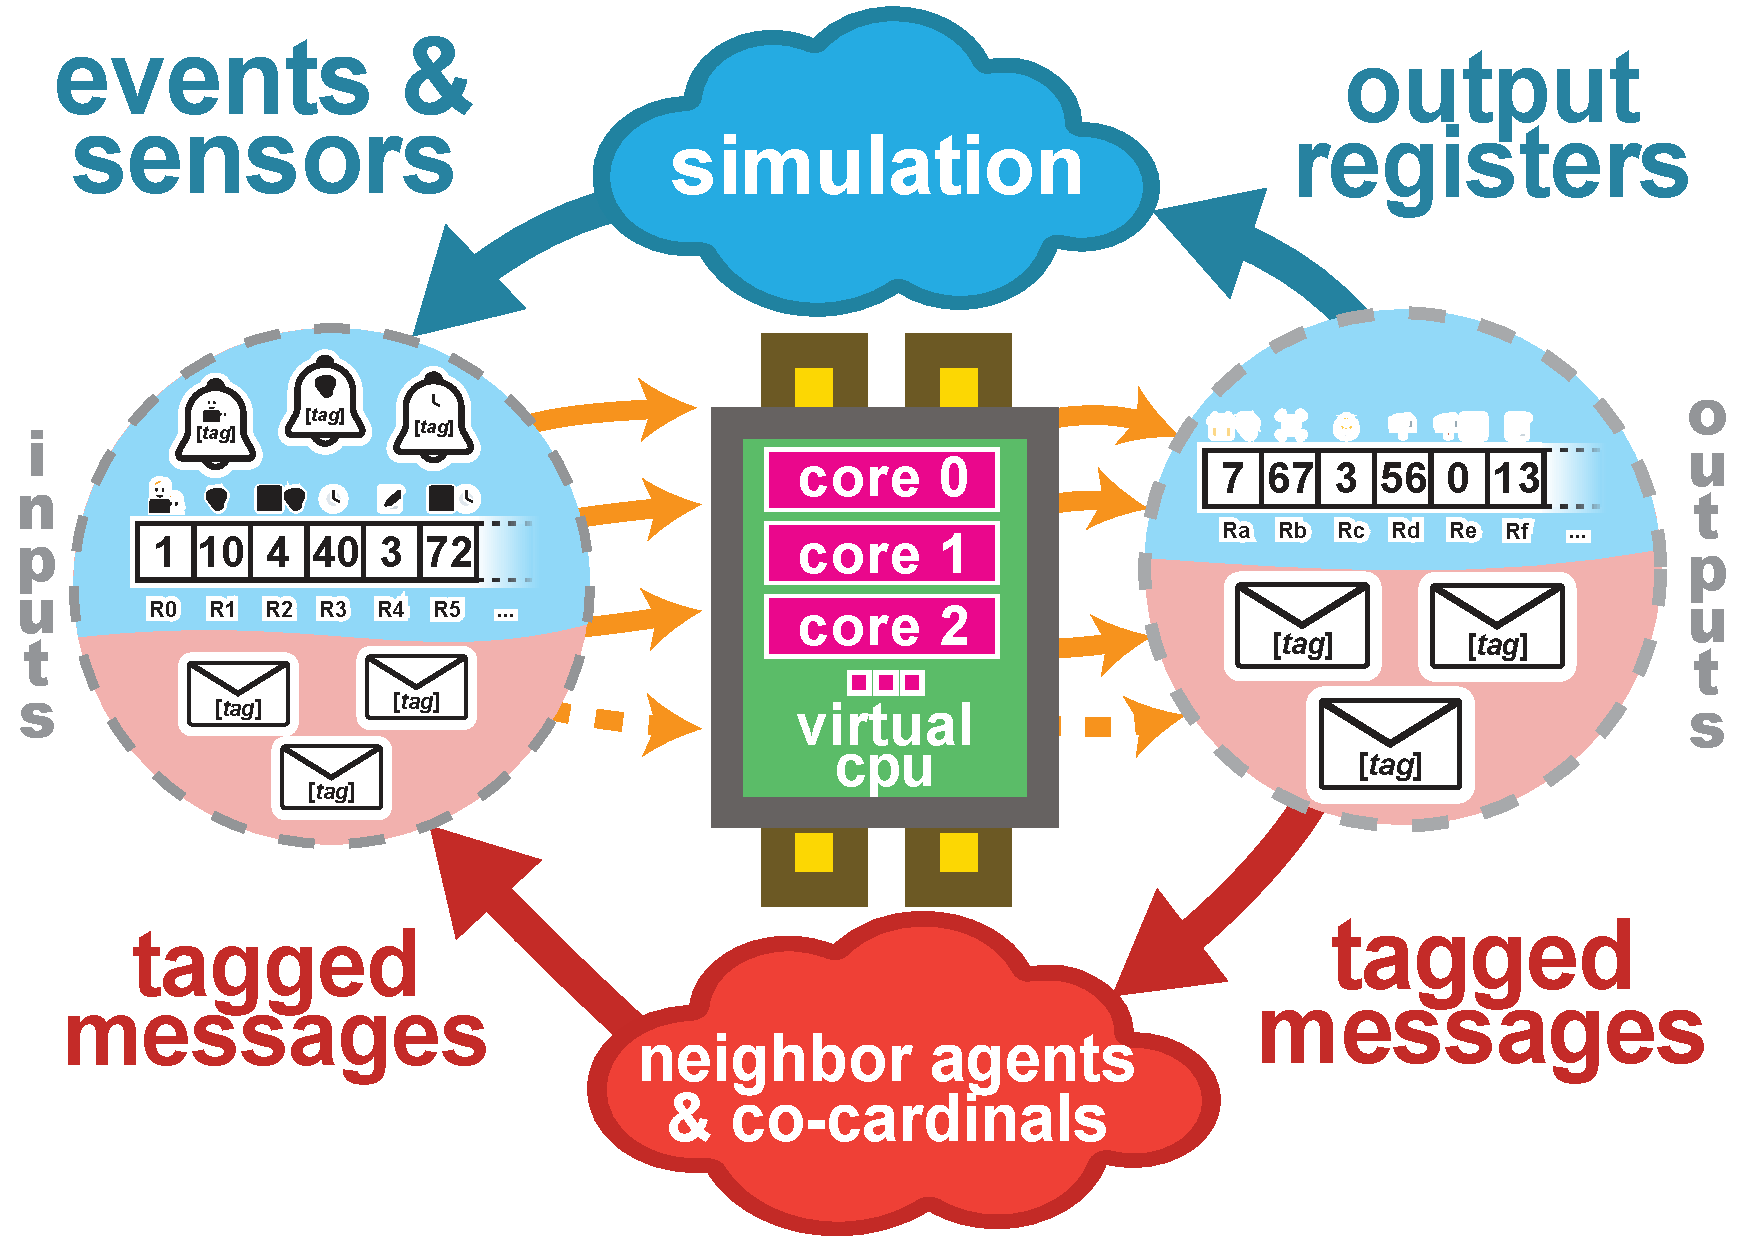
\includegraphics[width=\linewidth]{{img/cpu_detail}}

\caption{ \footnotesize
Overview of genome execution.
Tagged events and messages (shown as bells and envelopes, respectively) activate module execution on virtual cores.
Simulation state can also be read directly using sensor instructions to access input registers.
Special instructions write to output registers, allowing interaction with the simulation, and generate tagged messages, allowing interaction with other virtual CPUs.
}
\label{fig:cpu_detail}
\end{figure}


\begin{figure*}

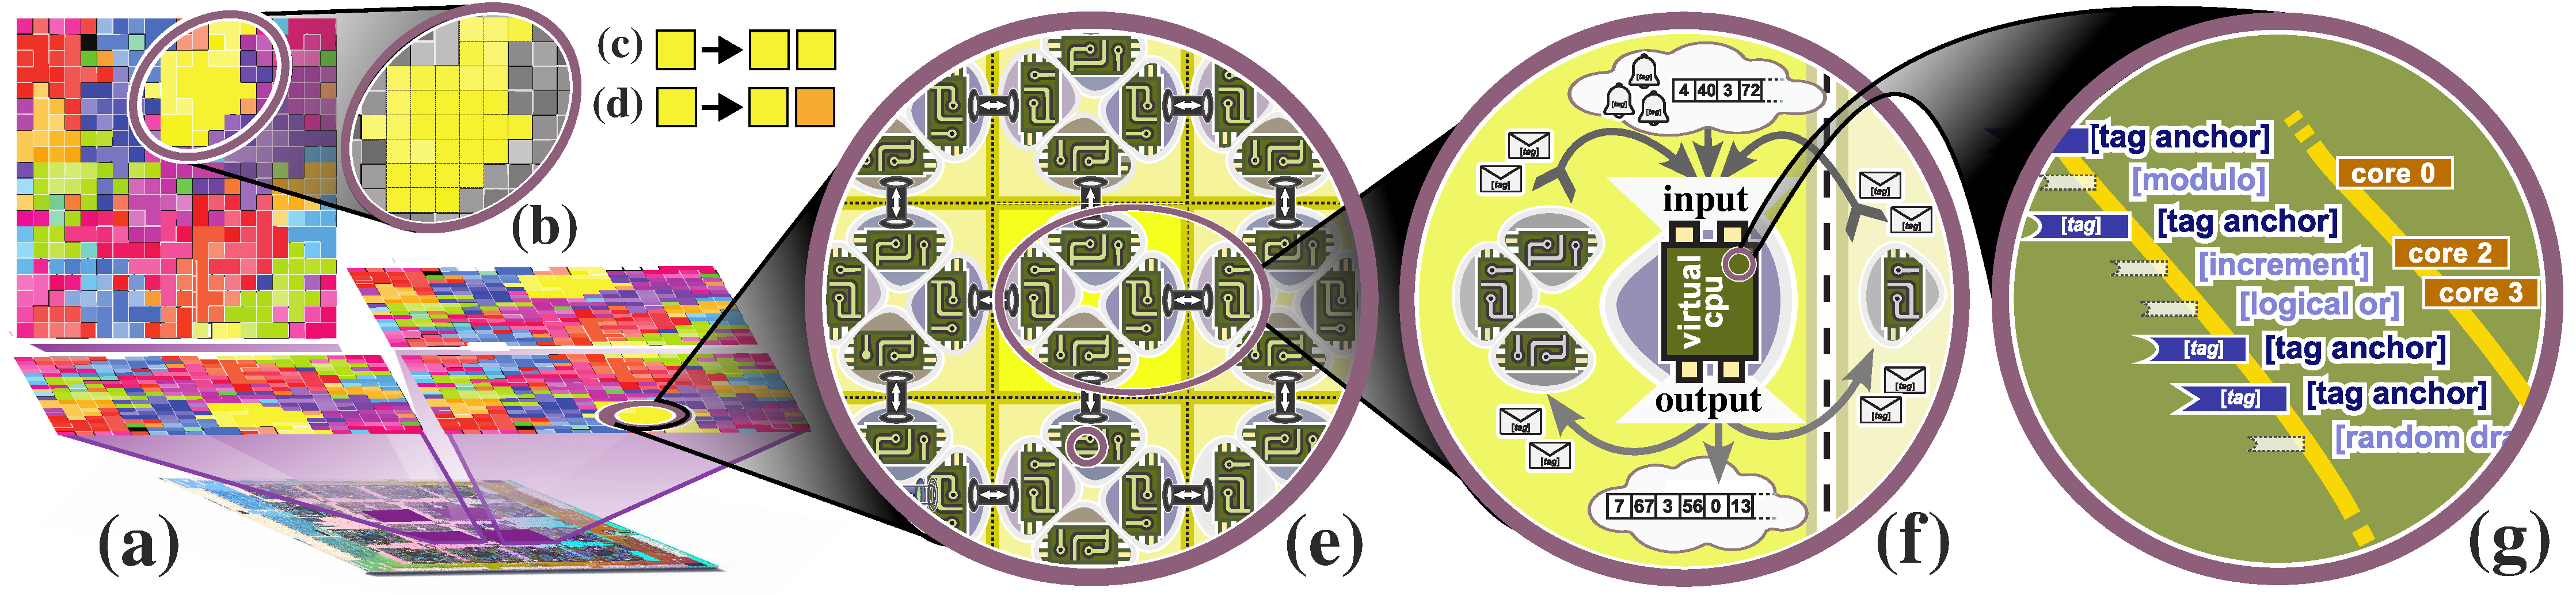
\includegraphics[width=\linewidth]{{img/graphic-oee4-cpu.pdf}}

\caption{
\textbf{Overview of digital multicell model.}
\footnotesize
Population comprises a toroidal grid of cells occupied by replicating computer programs.
In the surveyed case study, grid size was 14,400 cells ($120\times120$).
To accelerate the feasible evolutionary depth of experiments, population subgrids are evaluated across available hardware threads and processes --- in this work, 4 threads (panel $a$).
At subgrid boundaries where inter-cell interactions reach between different threads or processes, communication is handled on a best-effort basis via the underlying Conduit library.
On the population grid, cells may form local multicell groups --- shown as colored patches in visualizations (panel $b$).
Cells replicate by copying program content into a chosen neighbor cell, and may choose to grow their existing multicell group ($c$) --- or splinter their offspring off to found a new group ($d$).
Within each cell, behavior is directed by a collection of four virtual CPUs (N, S, E, and W ``cardinals''), each independently managing the cell's interactions with a one neighbor cell (panel $c$).
Each cardinal can interact with other cardinals in its own cell via message passing.
A cardinal can also exchange messages with its counterpart cardinal in the abutting neighbor cell, allowing arbitrary inter-cell communication.
Alongside message-passing I/O, cardinals accept input to sense local simulation state and create output to perform cell actions (panel $f$).
Sensory input occurs via a combination of special input registers (e.g., for own- and neighbor-cell resource availability, cell age, etc.) and special messages triggered by simulation conditions (``events,'' depicted as bells in panel $f$).
Behavior outputs are dispatched via special output registers (e.g., for resource sharing, replication, apoptosis, etc.).
At implementation level, replicator program code is evaluated via an event-driven execution model.
That is, tag-matching mechanisms trigger program submodules in response to stimuli (panel $g$).
In addition to external stimuli (i.e., inter-cellular messages, intra-cellular messages, and simulation events), program code can also trigger arbitrary self-stimuli.
Virtual hardware supports concurrent interaction handling via independent pseudo-cores, as well as dynamic plasticity through regulation of tag-matching affinities within each cardinal.
}
\label{fig:overview}
\end{figure*}


The DISHTINY simulation environment tracks cells occupying tiles on a $120\times120$ toroidal grid.
Cells collect a uniform inflow of continuous-valued resource.
This resource can be spent in increments of $1.0$ to attempt asexual reproduction into any of a cell's four adjacent cells.
A cell can only be replaced if it commands less than $1.0$ resource.
If a cell rebuffs a reproduction attempt, its resource stockpile decrements by $1.0$.

In order to facilitate the formation of coherent multicellular groups, the DISHTINY framework provides a mechanism for cells to form groups and detect group membership \citep{moreno2019toward}.
Groups arise through cellular reproduction.
When a cell proliferates, it may choose to initiate its offspring as a member of its kin group, thereby growing it, or induce the offspring to found a new kin group.
This process is similar to the growth of biological multicellular tissues, where cell offspring can be retained as members of the tissue or permanently expelled.

We incentivize group formation by providing an additional resource inflow bonus based on group size.
Groups that are too small do not receive this bonus.
Group that are too large receive a penalty.
In order to ensure group turnover, we force groups to fragment into unicells after 8,192 updates.

% Like physical attachment in biology, these kin groups do not in and of themselves  with respect to functional individuality.
% That is, the formation of kin groups doesn't necessarily imply that constituent cells are acting as a cohesive multicellular organism (TODO cite)--- it is necessary to test for traits characteristic of multicellularity such as cooperation, coordination, and reproductive division of labor.

In previous work, we established that this framework can select for traits characteristic of multicellularity, such as cooperation, coordination, and reproductive division of labor \cite{moreno2021exploring}.
We also found more case studies of interest arose when two nested levels of group membership were tracked
as opposed to a single, un-nested level of group membership \cite{moreno2021exploring}.
With nested group membership, group growth still occurs by cellular reproduction.
However, cells are given the choice to expel offspring from the innermost group (but retain membership in the outermost group) in addition to choosing to retain offspring within both groups or to expel offspring from both groups.
In this work, we allow for nested kin groups.

In addition to controlling reproduction behavior, evolving genomes can also share resources with adjacent cells, perform apoptosis (recovering a small amount of resource that may be shared with neighboring cells), and pass arbitrary messages to neighboring cells.
Cell behaviors are controlled by event-driven genetic programs in which linear GP modules are activated in response to cues from the environment or neighboring agents; signals are handled in quasi-parallel on up to 32 virtual cores (Figure \ref{fig:cpu_detail}) \citep{lalejini2018evolving}.
Each cell contains four independent virtual CPUs, all of which execute the same genetic program (Figure \ref{fig:overview}a).
Each CPU manages interactions with a single neighboring cell.
We refer to a CPU managing interactions with a particular neighbor as a ``cardinal'' (as in ``cardinal direction'').
These CPUs may communicate via intra-cellular message passing.
Full details on the instruction set and event library used as well as simulation logic and parameter settings appear in supplementary material.

\subsection{Evolution}
\label{sec:evolution;ch:measuring-cna}

We performed evolution in three hour windows for compatibility with our compute cluster's scheduling system.
We refer to these windows as ``stints.''
One-hundred instruction genomes were randomly generated at the outset of the initial stint, stint 0.
At the end of each three hour window, genomes were harvested and stored in a population file.
Subsequent stints were then seeded with the previous stint's population.
No simulation state besides genome content was preserved between stints.

In order to ensure heterogeneity of biotic environmental factors experienced by evolving cells, we imposed a diversity maintenance scheme.
In this scheme, descendants of a single progenitor cell from stint 0 that proliferated to constitute more than half of the population were penalized with resource loss.
The severity of the penalty increased with increasing prevalence beyond half of the population.
Thus, we ensured that descendants from at least two distinct stint 0 progenitors remained over the course of the simulation.
We arbitrarily chose the strain with the lowest integer root ID for primary study --- we refer to this strain as the ``focal'' strain and others as ``background'' strains.
(In our case study, there was only one background strain.)

In our screen for case studies, we evolved 40 independent populations for 101 stints.
We selected population 16005 from among these 40 to profile as a case study due to its distinct asymmetrical group morphology.

At the conclusion of each stint, we selected the most abundant genome within the population as a representative specimen.
We performed a suite of follow-up analyses on each representative specimen to characterize aspects of complexity, detailed in the following subsections.
To ensure that specimens were consistently sampled from descendants of the same stint 0 progenitor, we only considered genomes with the lowest available stint 0 progenitor ID.

\subsection{Phenotype-neutral Nopout}
\label{sec:phenotype_neutral_nopout}

After harvesting representative specimens from each stint, we began filtered out genome instructions that had no impact on the simulation.

To accomplish this, we performed sequential single-site ``nopouts'' where individual genome instructions were disabled by replaced with a \texttt{Nop} instruction.
\footnote{
This \texttt{Nop} instruction was chosen to perform the same number of random number generator touches as the original instruction to control for arbitrary effects of advancing the generator.
}
We reverted nopouts that altered a strain's phenotype and kept those that did not.
To determine whether phenotypic alteration occurred, we seeded an independent, mutation-disabled simulation with the stain in question and ran it side-by-side with an independent, mutation-disabled simulation of the wildtype strain.
If any divergence in resource concentration was detected between the two strains within a 2,048 update window, the single site nopout was reverted.
We continued this process until no single-site nopouts were possible without altering the genome's phenotype.
To speed up evaluation, we performed step-by-step, side-by-side comparisons using a smaller toroidal grid size of just 100 tiles.

This process left us with a ``Phenoytpe-neutral Nopout'' variant of the wildtype genome where all remaining instructions contributed to the phenotype.
%We called the number of remaining instructions in this skeleton genome its ``phenotype complexity.''

However, in further analyses we discovered that 21 phenotype-neutral nopouts from our case study were \textit{not} actually neutral --- competition experiments revealed they were significantly less fit than the wildtype strain.
This might be due to insufficient spatial or temporal scope to observe expression of particular genome sites in our test for phenotypic divergence.
%or effects of an instruction on the mutation.

\subsection{Estimating Critical Fitness Complexity}

Next, we sought to detect genome instructions that contributed to a strain's fitness.

For each remaining op instruction in the Phenotype-neutral Nopout variant, we took the wildtype strain and applied a nopout at the corresponding site.
We then competed this variant against the wildtype strain.
Only evaluating remaining op instructions in the Phenotype-neutral Nopout variant allowed us to decrease the number of fitness competitions we had to perform.

Fitness competitions began by seeding a population half-and-half with two strains.
These competitions ran for 10 minutes (about 4,200 updates) on a $60\times60$ toridal grid after which the simulation was ended and the relative abundances of descendants of both seeded strains were assessed.

To determine whether fitness differed significantly between a wildtype and variant strain, we compared the relative abundance of the strains observed at the end of competitions against outcomes from 20 control wildtype-vs-wildtype competitions.
We fit a $T$-distribution to the abundance outcomes observed under the control wildtype-vs-wildtype competitions and deemed outcomes that fell outside the central 98\% probability density of that distribution a significant difference in fitness.
This allowed us to screen for fitness effects of single-site nopouts while only performing a single competition per site.

This process left us with a ``Fitness-noncritical Nopout'' variant of the wildtype genome where all remaining instructions contributed to the phenotype.
We called the number of remaining instructions its ``critical fitness complexity.''
We adjusted this figure downwards for the expected 1\% rate of false-positive fitness differences among tested genome sites.
This metric mirrors the MODES complexity metric described in \citep{dolson2019modes} and the approximation of sequence complexity advanced in \citep{adami2000evolution}.

% \subsection{Estimating Interpolated Fitness Complexity}

% Single-instruction nopouts  reveal sites that are critical to fitness, but are insufficient to reveal all sites that contribute to fitness.
% For example, when instructions or modules are necessary but functionally redundant, disabling only one at a time will not discover their contribution to fitness.
% Indeed, we discovered that in 97 out of the 101 representative specimens analyzed, the Fitness-noncritical Nopout variant was significantly less fit than wildtype --- clearly noncritical sites also were contributing to fitness.

% Ideally, in order to whittle down to a  ``Fitness-neutral nopout'' skeleton, we would perform a Jenga-like procedure similar to that used to arrive at the ``Phenotype-neutral nopout''.
% However, because fitness is implicit in this simulation system and must be assessed statistically through competition experiments, it is costly to assess and cannot be determined with perfect reliability.
% (Playing a large game of Jenga to completion becomes intractable if attempting to remove a piece takes more than a few seconds or you can remove a critical piece early on without realizing it.)

% Instead, we used a sampling approach and statistical inference to estimate the number of noncritical genome sites that contribute to fitness.
% We focused on the role of the $n$ instructions that were present in a strain's phenotype-neutral nopout and but absent in its fitness-noncritical nopout.
% We performed 50 fitness competitions.
% Each competition $i$ was held between a wildtype genome and the phenotype-neutral nopout with with $h_i=i\times n/50$ randomly chosen additional noncritical instructions nopped out.
% This allowed us to sample the genome space interpolated between the phenotype-neutral nopout and the fitness-noncritical nopout.

% We modeled the occurrence of deleterious fitness effect as drawing any complete set of $s$ cards from a deck totaling $n$ cards with $m$ distinct sets shuffled in among them.
% In this model, a deleterious effect manifests when a set of $s$ specific sites are nopped out together.
% The model allows for $m$ independent available sets, any of which could cause a deleterious fitness effect.
% The probability $p_d(n,m,s,h)$ of a deleterious outcome (nopping at least one complete set of interacting sites) for a specific value of $m$, $n$, and $s$ given that $h$ sites have been nopped out can be calculated exactly through a recursive formula (Supplementary Listing \ref{lst:probability_deleterious}).

% For each sampled competition, we observed either a deleterious or a neutral outcome.
% The probability of the $i$th outcome with $h_i$ sites nopped is
% \begin{align*}
% p_i(m,s) =
% \begin{cases}
%     p_d(n,m,s,h_i) & \text{if deleterious}\\
%     1 - p_d(n,m,s,h_i) & \text{if neutral}
% \end{cases}
% \end{align*}

% We can calculate the likelihood of the particular set of 50 outcomes we observed given an underlying number of sets $m$ and set size $s$ as $\prod_i p_i(m,s)$.
% This formula allows us to find the values of $m$ an $s$ that maximize likelihood and best explain our observed data.

% To our surprise, we found that in most instances a set size $s$ of 1 gave higher likelihoods of the observed data than larger set sizes.
% It appears that the redundancy that prevented these sites from being detected in the fitness-critical nopout was eliminated by the phenotype-neutral nopout.
% In the future, it may be practical to couple this approach with a exhaustive battery single-site nopouts on sites present in a strain's phenotype-neutral nopout and but
% %todo which word? and or but?
% absent in its fitness-noncritical nopout.
% However, for parsimony's sake for all further analyses in this work we fixed $s=1$.

% We took the value $m$ that gave maximum likelihood of observed interpolation competition outcomes as the estimate for the number of noncritical instructions that contribute to fitness.
% We called this ``interpolated fitness complexity.''
% (Noncritical fitness complexity might be a better term for this metric moving forward, however.)
% We used the range of $m$ that accounts for the central 95\% of likelihood density to construct a 95\% credible interval for this metric.

% However, we were unable to perform this estimate because in 21 phenotype-neutral nopouts were significantly less fit than wildtype.
% %todo fix this sentence; not sure what it should say

\subsection{Estimating State Interface Complexity}
\label{sec:estimating-state-interface-complexity;ch:measuring-cna}

In addition to estimating the number of genome sites that contribute to fitness, we were interested in measuring the number of different environmental cues and the number of different output mechanisms that cells adaptively incorporated into behavior.

One possible way to take this measure would be to disable event cues, sensor instructions, and output registers one by one and test for changes in fitness.
However, this approach would fail to distinguish context-dependent input/output from merely contingent input/output.
For example, a cell might happen to depend on a sensor being set at a certain frequency but not on the actual underlying simulation information the sensor represents.

To isolate context-dependent input/output state interactions, we tested the fitness effect of swapping particular input/output states between CPUs rather than completely disabling them.
That is, for example, CPU $b$ would be forced to perform the output generated by CPU $a$ or CPU $b$ would be shown the input meant for CPU $a$.
We performed this manipulation on half the population in a fitness competition for each individual component of the simulation's introspective state (44 sensor states relating to the status of a CPU's own cell), extrospective state (61 sensor states relating to the status of a neighboring cell), and writable state (18 output states, 10 of which control cell behavior and 8 of which act as global memory for the CPU).
\footnote{
A full description of each piece of introspective, extrospective, and writable state is listed in supplementary material.
}
We deemed a state as fitness-critical if this manipulation resulted in decreased fitness at significance $p < 0.01$ using a $T$-test parameterized by 20 control wild-type vs wild-type competitions.

We describe the number of states that cells interact with to contribute to fitness as ``State Interface Complexity.''

\subsection{Estimating Messaging Interface Complexity}
\label{sec:estimating-messaging-interface-complexity;ch:measuring-cna}

In addition to estimating the number of input/output states cells use to interact with the environment, we were interested in estimating the number of distinct intra-cellular messages cardinals within a cell use to coordinate and inter-cellular messages that cells use to coordinate.
As with state interface complexity, distinguishing context-dependent behavior from contingent behavior is critical to attaining a meaningful measurement.
For example, a cardinal might happen to depend on always receiving a inter-cellular message from a neighbor or an intra-cellular message from another cardinal.
Although meaningless, if that message were blocked fitness would decrease.
So, instead of simply discarding messages to test for a fitness effect, we re-route messages back to the sending cardinal instead of their intended recipient.
We deemed a messages as fitness-critical if this manipulation resulted in decreased fitness at significance $p < 0.01$ using a $T$-test parameterized by 20 control wild-type vs wild-type competitions.

We refer to the number of distinct messages that cells send to contribute to fitness as ``Messaging Interface Complexity.''

We refer to the sum of State Interface Complexity, Intra-messaging Interface Complexity, and Inter-messaging Interface Complexity as ``Cardinal Interface Complexity.''

\subsection{Estimating Adaptation}
\label{sec:measuring-adaptation;ch:measuring-cna}

In order to assess ongoing changes in fitness, we performed fitness competitions between the representative focal strain specimen sampled at each stint and the focal strain population from the preceding stint.
(Recall from Section \ref{sec:evolution;ch:measuring-cna} that, due to a diversity maintenance procedure, two completely independent strains coexisted over the course of the experiment --- the ``focal'' strain selected for analysis and a ``background'' strain.)
Using the population, rather than the representative specimen, from the preceding stint as the competitive baseline ensured more focused, consistent measurement of the fitness properties of the specimen at the current stint (e.g., preventing skewed results from a sampled ``dud'' at the preceding stint).

We performed 20 independent replicates of each competition.
Competing strains were well-mixed within the full-sized toroidal grid at the outset of each competition, which lasted for 10 minutes of wall time.
This was sufficient to simulate about 8,000 updates at stint 0 and 2,000 updates at stint 100 (Supplementary Figures \ref{fig:num_updates_elapsed_heatmap}, \ref{fig:num_updates_elapsed_barplot}, and \ref{fig:num_updates_elapsed_boxplot}).
We determined that a gain of fitness had occurred if the current stint specimen constituted a population majority at the conclusion of more than 17 of those competitions, corresponding to a significance level of $p < 0.005$ under the two-tailed binomial null hypothesis.
Likewise, we deemed winning fewer than 3 competitions a significant fitness loss.


\subsection{Implementation}

Multithreading was employed to speed up execution.
We broke the simulation into four $60\times60$ subgrids.
Each subgrid executed asynchronously, using the Conduit C++ Library to orchestrate best-effort, real-time interactions between simulation elements on different threads.
This approach is inspired by Ackley's notion of indefinite scalability \citep{ackley2014indefinitely}.
In other work benchmarking the system, we have demonstrated that this approach improves scalability.
The simulation scales to 4 threads with 80\% efficiency, up to 64 threads with 40\% efficiency and up to 64 nodes with 80\% efficiency \citep{moreno2021conduit}.
%TODO multicellular between distribute dsystems We are excited about the potential of the system not just

% https://mybinder.org/v2/gh/mmore500/dishtiny/e17e6d5e258b7aacac72d44922008ab14e80e182?filepath=binder%2Fbucket%3Dprq49%2Fa%3Dall_stints_all_series_profiles%2Bendeavor%3D16%2Fcase_study_16005.ipynb
Over the 101 three-hour evolutionary stints performed to evolve the case study, 7,565,309 simulation updates elapsed.
(This translates to 74,904 updates elapsed per stint or about 6.9 updates per second.)
However, the update processing rate was not uniform across stints: the simulation slowed about 77\% as stints progressed.
Supplementary Figure \ref{fig:simulation} shows elapsed updates for each stint.
During stint 0, 176,816 updates elapsed (about 16.3 updates per second).
During stint 100, only 41,920 updates elapsed (about 3.8 updates per second).

% https://mybinder.org/v2/gh/mmore500/dishtiny/e17e6d5e258b7aacac72d44922008ab14e80e182?filepath=binder%2Fbucket%3Dprq49%2Fa%3Dall_stints_all_thread_profiles%2Bendeavor%3D16%2Felapsed_updates.ipynb
Although working asynchronously, threads processed similar number of updates during each stint.
The mean standard deviation of update-processing rate between threads was 2\%.
The mean difference of the update-processing rate between the fastest and slowest threads was 5\%.
The maximum value of these statistics observed during a stint was 9\% and 20\%, respectively, at stint 44.
Supplementary Figure \ref{fig:simulation:thread_updates} shows the distribution of elapsed updates across threads for each stint evolved during the case study.

Software is available under a MIT License at \url{https://github.com/mmore500/dishtiny}.
All data is available via the Open Science Framework at \url{https://osf.io/prq49}.
Supplementary material is available via the Open Science Framework at \url{https://osf.io/gekc8}.
%TODO dependencies


\section{Results}

\subsection{Evolutionary History}

% https://mybinder.org/v2/gh/mmore500/dishtiny/e17e6d5e258b7aacac72d44922008ab14e80e182?filepath=binder%2Fbucket%3Dprq49%2Fa%3Dall_stints_all_series_profiles%2Bendeavor%3D16%2Fcase_study_16005.ipynb
Due to the parallel nature of the experimental framework, we did not perform perfect phylogeny tracking.
However, we did track the total number of ancestors seeded into stint 0 with extant descendants.
At the end of stints 0 and 1, three distinct original phylogenetic roots were present in the population.
From stint 2 onward, only two distinct original phylogenetic roots were present.

% https://mybinder.org/v2/gh/mmore500/dishtiny/e17e6d5e258b7aacac72d44922008ab14e80e182?filepath=binder%2Fbucket%3Dprq49%2Fa%3Dall_stints_all_series_profiles%2Bendeavor%3D16%2Fcase_study_16005.ipynb
We performed follow-up analyses on specimens sampled from the lowest original phylogenetic root ID present in the population.
For the first two stints, this was root ID 2,378.
During stint 2, original phylogenetic root 2,378 went extinct.
So, all further follow-up analyses were sampled from descendants of ancestor 12,634.

We also tracked the number of genomes reconstituted at the outset of each stint with extant descendants at the end of that stint.
This count grows from approximately 10 around stint 15 to upwards of 30 around stint 40 (Supplementary Figure \ref{fig:phylogeny:stint_roots}\citep{Moreno_2021}).
Among descendants of the lowest original phylogenetic root, the number of independent lineages spanning a stint also increases from around 5 to around 15
(Supplementary Figure \ref{fig:phylogeny:lowestroot_stint_roots} \citep{Moreno_2021}).
This decrease in phylogenetic consolidation on a stint-by-stint basis correlates with the waning number of simulation updates performed per stint (Supplementary Figures \ref{fig:phylogeny:updates_vs_stint_roots} and \ref{fig:phylogeny:log_updates_vs_stint_roots} \citep{Moreno_2021}).
More complete phylogenetic data will be necessary in future experiments to address questions about the possibility of long-term stable coexistence beyond the two strains supported under the explicit diversity maintenance scheme.

% https://mybinder.org/v2/gh/mmore500/dishtiny/e17e6d5e258b7aacac72d44922008ab14e80e182?filepath=binder%2Fbucket%3Dprq49%2Fa%3Dall_stints_all_series_profiles%2Bendeavor%3D16%2Fcase_study_16005.ipynb
On the specimen from stint 100 used in the final case study, an evolutionary history of 20,212 cell generations had elapsed.
Of these cellular reproductions, 11,713 (58\%) had full kin group commonality, 7,174 had partial kin group commonality (35\%), and 1,325 had no kin group commonality (7\%).
On this specimen, 1,672 mutation events had elapsed.
During these events, 7,240 insertion-deletion alterations had occurred and 26,153 point mutations had occurred.
This strain experienced a selection pressure of 18\% over its evolutionary history, meaning that only 82\% of the mutations that would be expected given the number of cellular reproductions that had elapsed were present.

\begin{figure*}
\centering
\includegraphics[width=0.8\linewidth]{{submodule/dishtiny_event_tag_phylogenetics/teeplots/ladderized_parsimony_tree_no_outliers/viz=draw+ext=}}

\caption{
\textbf{Estimated phylogeny of sampled focal strain representatives.}
\footnotesize
Phylogeny constructed using parsimony algorithm based on genome tag bitstring content \citep{cock2009biopython}.
Each leaf node corresponds to a sampled representative.
Representatives from stints 0 and 1, which share no common ancestry with representatives from other stints, are excluded.
Numbers refer to stint that each representative was sampled from.
Color coding and parentheticals of stint labels correspond to qualitative morph codes described in Table \ref{tab:morph_descriptions}.
}
\label{fig:phylo_parsimony_tree}
\end{figure*}


% https://github.com/mmore500/dishtiny_event_tag_phylogenetics/commit/ecc2ab8a580b125bea9f661e49cd4d7f34bfa1bb
In order to characterize the evolutionary history of the experiment in greater detail, we performed a parsimony-based phylogenetic reconstruction on the sampled representative specimens from each stint, shown in Figure \ref{fig:phylo_parsimony_tree}.
We used genomes' fixed-length blocks of 35 64-bit tags that mediate environmental interactions as the basis for this reconstruction.
These tag blocks underwent bitwise mutation over the course of the experiment.\footnote{
In future experiments, we plan to incorporate new methodology for ``Hereditary Stratigraph'' genome annotations expressly designed to facilitate phylogenetic reconstruction \citep{moreno2022hereditary}.
}
Supplementary Figure \ref{fig:phylo_distance_matrix_heatmap} shows hamming distance between all pairs of tag blocks.
We additionally tried several other tree inference methods, discussed in supplementary material; however, these yielded lower-quality reconstructions.

Although the phylogeny of stint representatives includes many instances breaking strict stint-on-stint ladderization (i.e., each stint's representative descending directly from the preceding stint's representative), we did not observe evidence of long-term coexistence of clades over more than ten stints.

\subsection{Qualitative Morphological Categorizations}

\input{lib/dissertationelse.tex}
\input{lib/dissertationexclude.tex}
\input{lib/dissertationonly.tex}

\newcommand{\includesnapshot}[1] {%
\adjustbox{trim={0.05\width} {0.35\width} {0.05\width} {0.35\width},clip}%
    {\includegraphics[height=\dissertationexclude{0.3}\dissertationonly{0.25}\textheight]{#1}}
}
\newcommand{\morphtext}[1] {%
\color[HTML]{FFFFFF} \huge \raisebox{1.2em}{\textbf{#1}}%
}
\newcommand{\videolink}[1] {%
\raisebox{
\dissertationexclude{2.8em}
\dissertationonly{2.2em}
}{\begin{minipage}{\dissertationelse{2.4cm}{1.3 cm}} \dissertationelse{\fontsize{6}{7}\selectfont}{\tiny}\url{#1} \end{minipage}}
}
\newcommand{\descript}[1] {%
\raisebox{
  \dissertationexclude{2.8em}
  \dissertationonly{2.2em}
}{\begin{minipage}{\linewidth}\dissertationonly{\fontsize{8}{8}\selectfont} #1 \end{minipage}}
}


{
\catcode`\%=12
\begin{table*}
\begin{tabular}{cp{0.4\textwidth}ll}
\multicolumn{1}{l}{\textbf{ID}}               & \textbf{Morphology} & \textbf{Snapshot} & \textbf{Video} \\
\cellcolor[HTML]{4C72B0}{ \morphtext{a} } & \descript{Individual cells, no multicellular kin groups. Resource use is low---most cells simply hoard resource until their stockpile is beyond sufficient to reproduce. Only a handful of cells intermittently expend resource.} & \includesnapshot{\detokenize{snapshots/sanitized/a=kin-group-id+idx=0+proc=0+series=16005+stint=0+thread=0+update=28991+ext=.png}}             &  \videolink{https://hopth.ru/21/b=prq49+s=16005+t=0+v=video+w=specimen}          \\
\cellcolor[HTML]{DD8452}{\morphtext{b}} & \descript{Mostly individual cells, with some two-, three-, and four-cell groups evenly spread out. Resource usage occurs in short spurts in one or two adjacent cells. } & \includesnapshot{\detokenize{snapshots/sanitized/a=kin-group-id+idx=0+proc=0+series=16005+stint=1+thread=0+update=14271+ext=.png}}                 & \videolink{https://hopth.ru/21/b=prq49+s=16005+t=1+v=video+w=specimen}              \\
\cellcolor[HTML]{55A868}{\morphtext{c}} & \descript{Large multicellular groups dominate, consisting of hundreds of cells. Group growth is unchecked and continues until cells' resource stockpiles are entirely depleted by the excess group size penalty.} & \includesnapshot{\detokenize{snapshots/sanitized/a=kin-group-id+idx=0+proc=0+series=16005+stint=2+thread=0+update=17471+ext=.png}}                  & \videolink{https://hopth.ru/21/b=prq49+s=16005+t=2+v=video+w=specimen}             \\
\cellcolor[HTML]{C44E52}{\morphtext{d}} & \descript{Clear groups of 10 to 15 cells form. Cell proliferation appears somewhat more active at the periphery of groups compared to the interior.} & \includesnapshot{\detokenize{snapshots/sanitized/a=kin-group-id+idx=0+proc=0+series=16005+stint=14+thread=0+update=16959+ext=.png}}                  & \videolink{https://hopth.ru/21/b=prq49+s=16005+t=14+v=video+w=specimen}               \\
\cellcolor[HTML]{8172B3}{\morphtext{e}} & \descript{Groups are visibly elongated along the horizontal axis. After initial development, some gradual, irregular growth occurs along the vertical axis.} & \includesnapshot{\detokenize{snapshots/sanitized/a=kin-group-id+idx=0+proc=0+series=16005+stint=15+thread=0+update=16639+ext=.png}}                  & \videolink{https://hopth.ru/21/b=prq49+s=16005+t=15+v=video+w=specimen}              \\
\cellcolor[HTML]{937860}{\morphtext{f}} & \descript{Groups are horizontally elongated similarly to morphology $e$, but have a larger consistent vertical thickness of three or four cells.} & \includesnapshot{\detokenize{snapshots/sanitized/a=kin-group-id+idx=0+proc=0+series=16005+stint=39+thread=0+update=10303+ext=.png}}                  & \videolink{https://hopth.ru/21/b=prq49+s=16005+t=39+v=video+w=specimen}             \\
\cellcolor[HTML]{DA8BC3}{\morphtext{g}} & \descript{Initial group growth is almost entirely horizontal, with groups usually taking up only one row of cells. However, after an apparent timing cue groups perform a brief bout of aggressive vertical growth.} & \includesnapshot{\detokenize{snapshots/sanitized/a=kin-group-id+idx=0+proc=0+series=16005+stint=45+thread=0+update=12991+ext=.png}}                  & \videolink{https://hopth.ru/21/b=prq49+s=16005+t=45+v=video+w=specimen}              \\
\cellcolor[HTML]{8C8C8C}{\morphtext{h}} & \descript{Groups grow horizontally and then proliferate vertically on a timing cue like morph $e$. However, after that timing cue cell proliferation is incessant with almost no resource retention.} & \includesnapshot{\detokenize{snapshots/sanitized/a=kin-group-id+idx=0+proc=0+series=16005+stint=59+thread=0+update=11839+ext=.png}}                  & \videolink{https://hopth.ru/21/b=prq49+s=16005+t=59+v=video+w=specimen}              \\
\cellcolor[HTML]{CCB974}{\morphtext{i}} & \descript{Irregular groups of mostly less than ten cells. Incessant proliferation with almost no resource retention leads to rapid group turnover.} & \includesnapshot{\detokenize{snapshots/sanitized/a=kin-group-id+idx=0+proc=0+series=16005+stint=74+thread=0+update=12991+ext=.png}}                  & \videolink{https://hopth.ru/21/b=prq49+s=16005+t=74+v=video+w=specimen}              \\
\cellcolor[HTML]{64B5CD}{\morphtext{j}} & \descript{
Groups grow horizontally and then proliferate vertically on a timing cue like morph $e$. However, several viable horizontal-bar offspring groups form before forced fragmentation.} & \includesnapshot{\detokenize{snapshots/sanitized/a=kin-group-id+idx=0+proc=0+series=16005+stint=100+thread=0+update=8767+ext=.png}}                  & \videolink{https://hopth.ru/21/b=prq49+s=16005+t=100+v=video+w=specimen}
\end{tabular}

\caption{
\textbf{Qualitative morph phenotype categorizations.}
\footnotesize
Color coding of morph IDs has no significance beyond guiding the eye in scatter plots where points are labeled by morph.
Snapshot visualizes spatial layout of kin groups on toroidal grid at a fixed point in time.
Each cell corresponds to a small square tile.
Color hue denotes, and black borders divide, outermost kin groups; color saturation denotes, and white borders divide, innermost kin groups.
}
\label{tab:morph_descriptions}

\end{table*}
}


We performed a qualitative survey of the evolved life histories along the evolutionary timeline by analyzing video recordings of monocultures of each stint's representative specimen.

Table \ref{tab:morph_descriptions} summarizes the ten morphological categories we grouped specimens into.
In brief, specimens from early stints largely grew as unicellular or small multicellular groups (morphs $a$, $b$).
Then, the specimen from stint 14 grew as larger, symmetrical groups (morph $d$).
At stint 15, a distinct, asymmetrical horizontal bar morphology evolved (morph $e$).
%todo structure above is confusing
% Consistently left/right, indicating that somehow broke symmetrical of the simulation.
At stint 45, a delayed secondary spurt of group growth in the vertical direction arose (morph $g$).
This morphology was sampled frequently until stint 60 when morph $e$ began to be sampled primarily again.
However, morph $g$ was observed as late as stint 90.

Phylogenetic analysis (Figure \ref{fig:phylo_parsimony_tree}) indicates that observations of morph $e$ at stint 53 and onward are instances of secondary loss rather than retention of trait $e$ by a separate lineage coexisting with the lineage expressing morph $g$.
Three separate reversion events from morph $g$ to morph $e$ appear likely.
Interestingly, morph $g$ individuals at stints 89 and 90 appear to represent subsequent trait re-gain after reversion from morph $g$ to morph $e$.

Table \ref{tab:morph_descriptions} provides more detailed descriptions of each qualitative morph category as well as video and a still image example of each.
Supplementary Table \ref{tab:morph_by_stint} provides morph categorization for each stint as well as links to view the stint's specimen in a video or in-browser web simulation \citep{Moreno_2021}.

% \subsection{Multicellular Phenotypic Traits}

% In order for a transition in individuality, cells have to diminish their own immediate reproductive interests in order to prioritize the interests of the collective.
% In previous work with an earlier version of the system, we've seen multicellular traits evolve such as (blah from abstract) %todo
% \citep{moreno2021exploring}.

% The formation of kin group morphologies in this system does not necessarily imply a transition in individuality.
% It is necessary to test to see if cells within groups are meaningfully cooperating.

% Because cell reproduction is necessarily adversarial in this system, we can test to see whether cells preferentially target or spare their group members.
% A conflict ratio of less than 1 implies that cells preferentially spare their members.
% We observed a  0.5 most of the time.

% Supplementary Figure \ref{fig:conflict:exactly_one} shows the  . %todo
% Supplementary Figure \ref{fig:conflict:at_least_one}
% Supplementary Figure \ref{fig:conflict:exactly_two}.
% However, could be an artifact of cell-offspring cooperation.

% Interestingly, this strain appears to be using ``Is Child Cell Of,'' ``Is Parent Cell Of,'' ``Is Child Group Of,'' and the raw kin group ID of neighbors (but not the raw kin group ID of self).

% %todo change wording, not sure what you're hoping to say with first phrase
% To more conclusively, in future work we plan to look at the reproductive output at the interior of multicellular groups to see if these cells diminish their own reproductive output and to control for cellular relatedness when calculating this element of group cooperation.

% We analyzed other traits characteristic of multicellularity, as well.

% We did not see widespread resource sharing over the evolutionary history.
% Only tiny fractions of cells, less than 1\%, appeared to share tiny amounts of the resource, less than 1\% of the resource required to reproduce per update (Supplementary Figures \ref{fig:resource_sharing:fraction_sharing_monoculture} and \ref{fig:resource_sharing:sharing_amount_monoculture}).
% However, in ten strains sampled along the evolutionary lineage, context-dependent resource-sending behavior contributed to fitness (Supplementary Figure \ref{fig:writable_perturbation}).
% Interestingly, another strain present in the population that was not the subject of analysis appeared to evolve widespread, higher-throughput resource sharing after stint 60 (Supplementary Figures \ref{fig:resource_sharing:fraction_sharing_evolve} and \ref{fig:resource_sharing:sharing_amount_evolve}).

% We observed widespread apoptosis over the evolutionary history.
% As shown in Supplementary Figure \ref{fig:apoptosis:apoptosis_stint}, in most monocultured representative strains, between 10 and 30\% of cell deaths were due to apoptosis.
% However, it is not clear if this apoptosis returned a fitness benefit.
% No context-dependent apoptosis behavior contributed to fitness for any sampled strain over the evolutionary history (Supplementary Figure \ref{fig:writable_perturbation}).
% It is unclear whether context-independent apoptosis might have a fitness benefit.

% The behavior seems like cells from within a group don't explicitly recognize one another according to group membership. However, they do recognize their cell parent/child and arrange themselves in a somewhat linear fashion that minimizes the potential for conflict between cells.
% Overall, there are elements of cooperation but is unclear to what extent this particular strain constitutes a proper fraternal transition in individuality.

\subsection{Fitness}

% \begin{figure}

\input{fig/fitness/fitness_neutrality.tex}
\input{fig/fitness/fitness_magnitude.tex}
\input{fig/fitness/doubling_time.tex}

\caption{ Fitness assays.
Color coding and letters correspond to qualitative morph codes described in Table \ref{tab:morph_descriptions}.
Dotted vertical line denotes emergence of morph $e$.
Dashed vertical line denotes emergence of morph $g$. }
\label{fig:fitness}

\end{figure}

\begin{figure*}

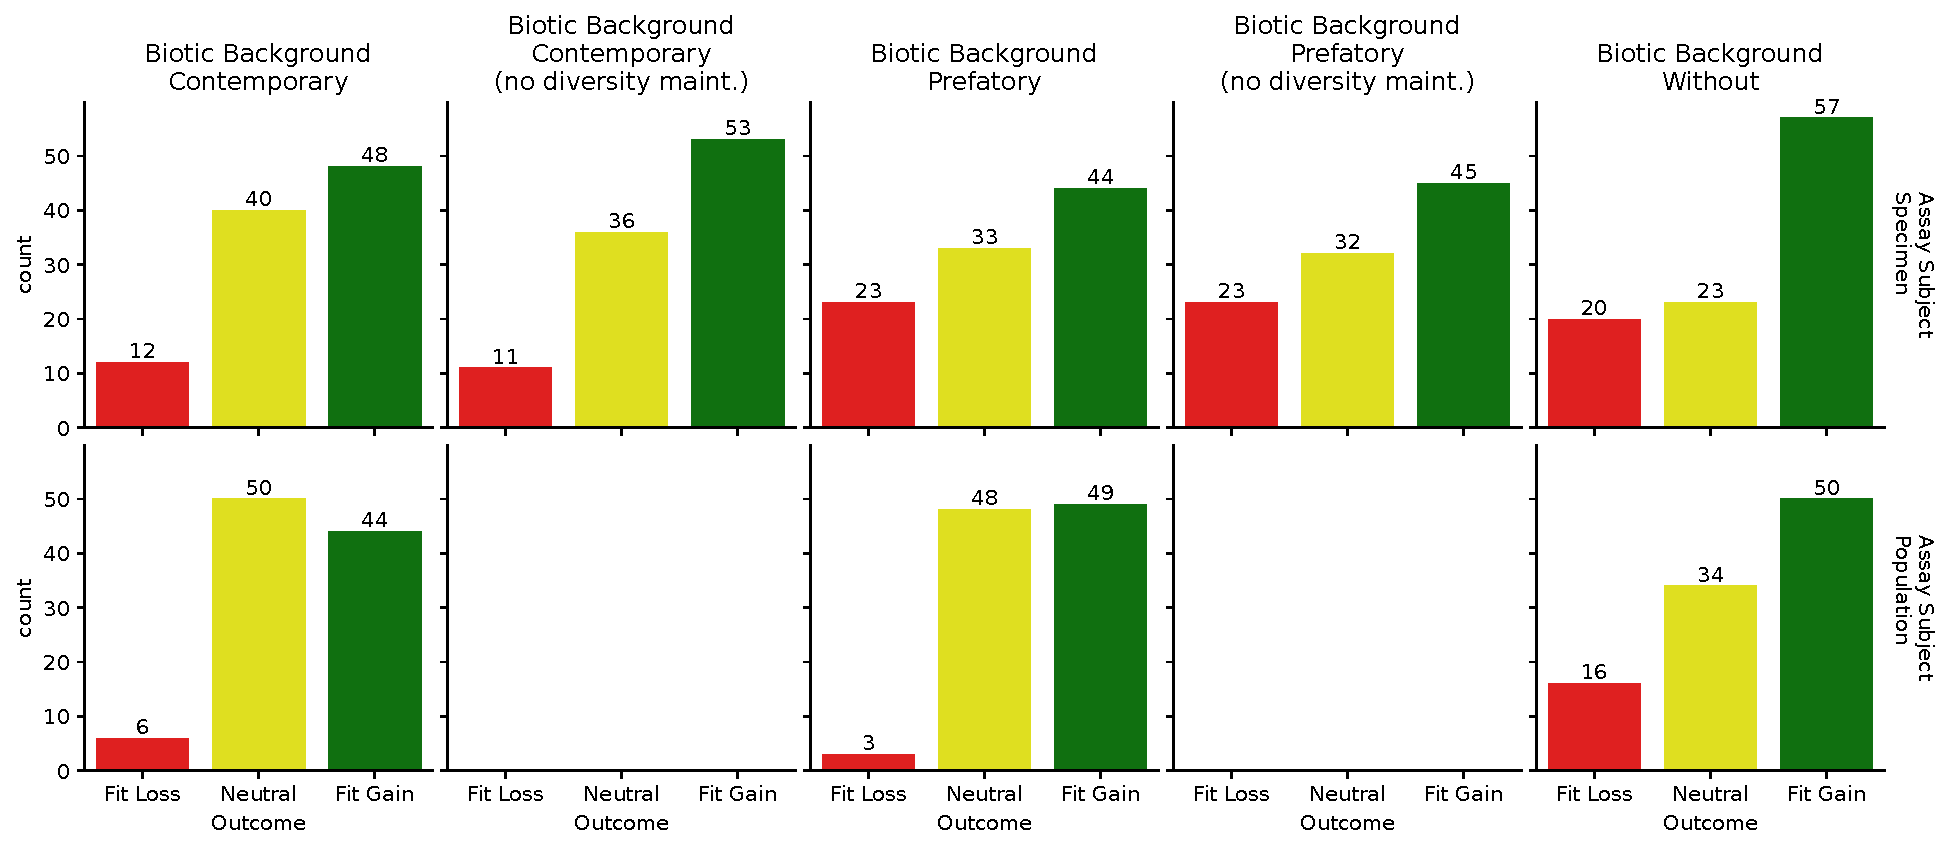
\includegraphics[width=\linewidth]{{submodule/dishtiny/binder/bucket=prq49/a=adaptation_assays+endeavor=16/teeplots/col=biotic-background+kind=count+row=assay-subject+viz=barlabel-catplot+x=outcome+ext=}}

\caption{
TODO
}
\label{fig:outcome_count_distns}
\end{figure*}


Of the 100 competition assays performed, 57 indicated significant fitness gain, 23 were neutral, and 20 indicated significant fitness loss (shown in upper right of Figure \ref{fig:outcome_count_distns}, at the intersection of the ``Biotic Background, Without'' column and ``Assay Subject, Specimen'' row.)

Surprised by the frequency of deleterious outcomes, we performed a second set of experiments to investigate whether these outcomes could be explained as sampling of ``dud'' representatives.
In these competition assays, we competed the entire focal strain population against the focal strain population from the preceding stint.
However, we observed a similar result: 50 assays indicated significant fitness gain, 34 were neutral, and 16 indicated significant fitness loss (shown in lower right of Figure \ref{fig:outcome_count_distns}, at the intersection of the ``Biotic Background, Without'' column and ``Assay Subject, Population'' row.)

\begin{figure*}
\centering
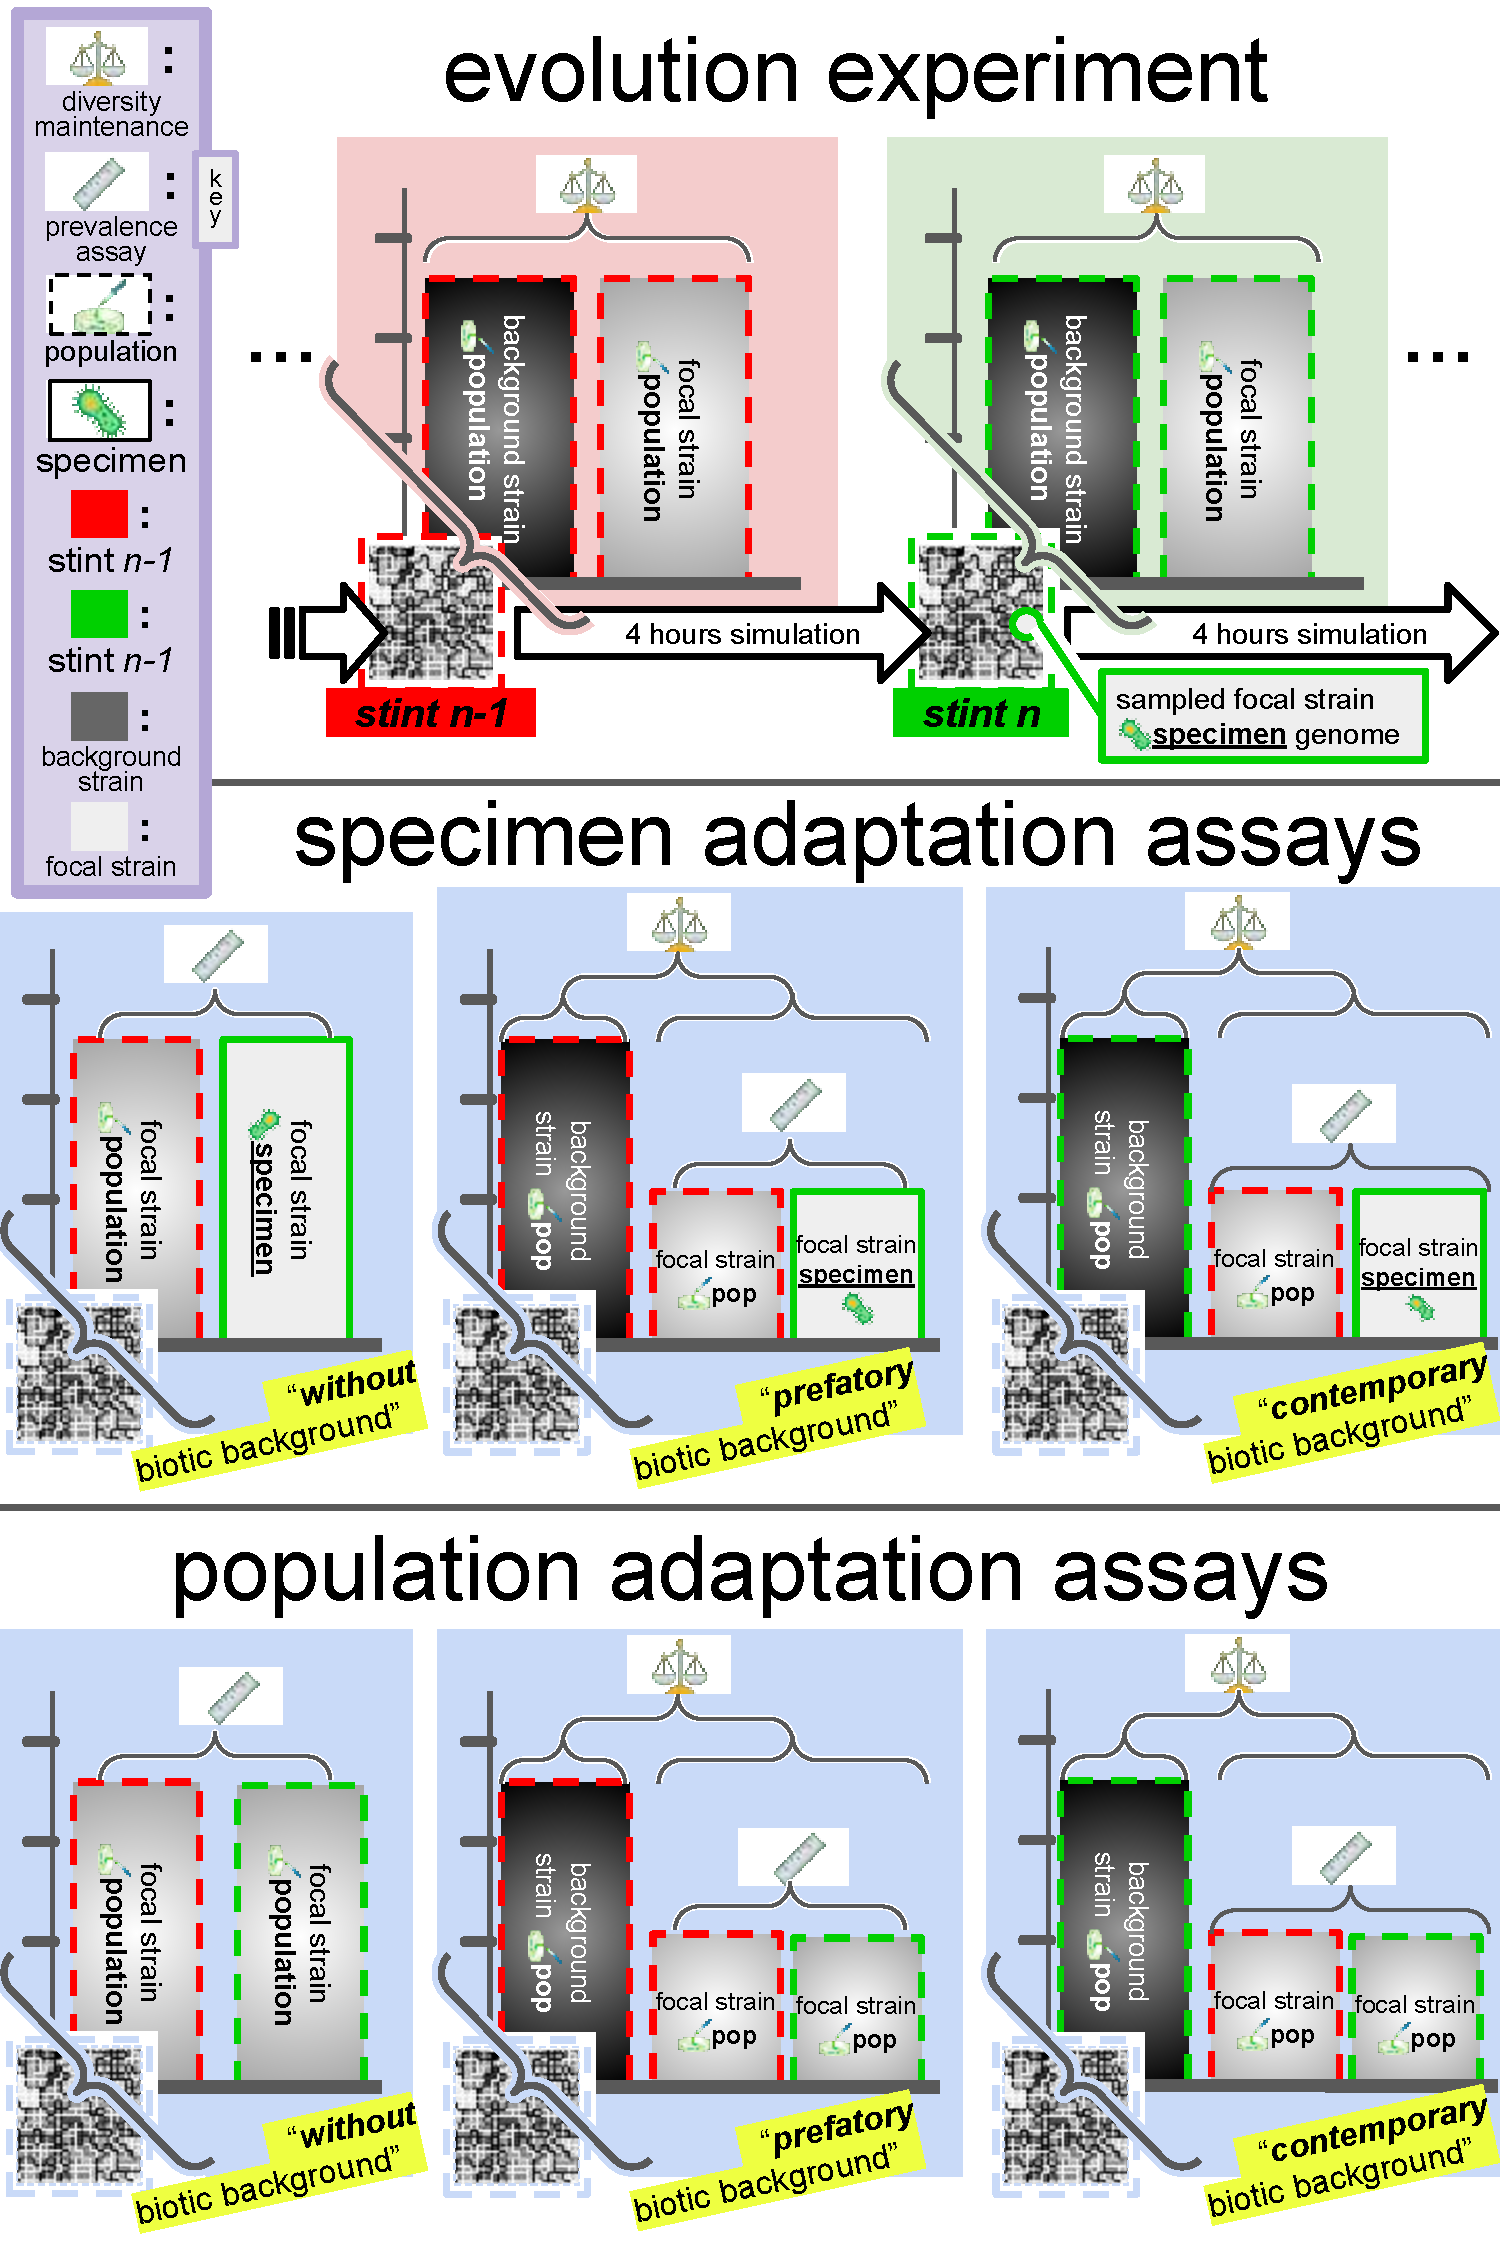
\includegraphics[width=0.5\linewidth]{{img/adaptation-assay-cartoon}}

\caption{
Detail of adaptation assay design.
Top panel shows progress of original evolutionary experiment over one stint.
A diversity maintenance procedure was used to ensure long-term coexistence of a least two strains over the course of the experiment by penalizing any strain that occupied more than half of thread-local population space.
A ``focal strain'' was arbitrarily chosen for study; we refer to the other strain as the ``background strain.''
Adaptation assays in lower panels measure fitness change over the course of that stint through against the population from the preceding stint.
The middle panel shows measurement of adaptation of the representative specimen that was sampled for analysis at each stint.
The bottom panel shows measurement of the adaptation of the entire focal strain population at each stint.
Competitors were mixed in even proportion into the environment.
Bar heights represent initial relative proportions of assay participants at the beginning of the competition.
Adaptation was measured by measuring change in population composition over a 10 minute competition window.
We call this measurement of population composition change a ``prevalence assay''.
Competition experiments were performed absent the background strain, with the background strain population from the preceding stint, or with the background strain population from the current stint --- shown separately in each panel.
}
\label{fig:adaptation_assay_cartoon}
\end{figure*}


Next, we investigated whether the presence of the background strain as a ``biotic background'' influenced fitness.
We repeated the two experiments described above (specimen and population competition assays), but inserted the background strain as half of the initial well-mixed population.
In one assay setup, we used the background strain population from the current stint.
We refer to this as ``contemporary biotic background.''
In another, which we call ``prefatory biotic background,'' we used the background strain population from the previous stint.
We refer to the original competition assays absent the background strain as ``without biotic background.''
Figure \ref{fig:adaptation_assay_cartoon} summarizes these competition assay designs.

\begin{sidewaysfigure*}
\thisfloatpagestyle{mylandscape}%
\rotatesidewayslabel%
\centering

\begin{subfigure}[t]{0.32\textwidth}
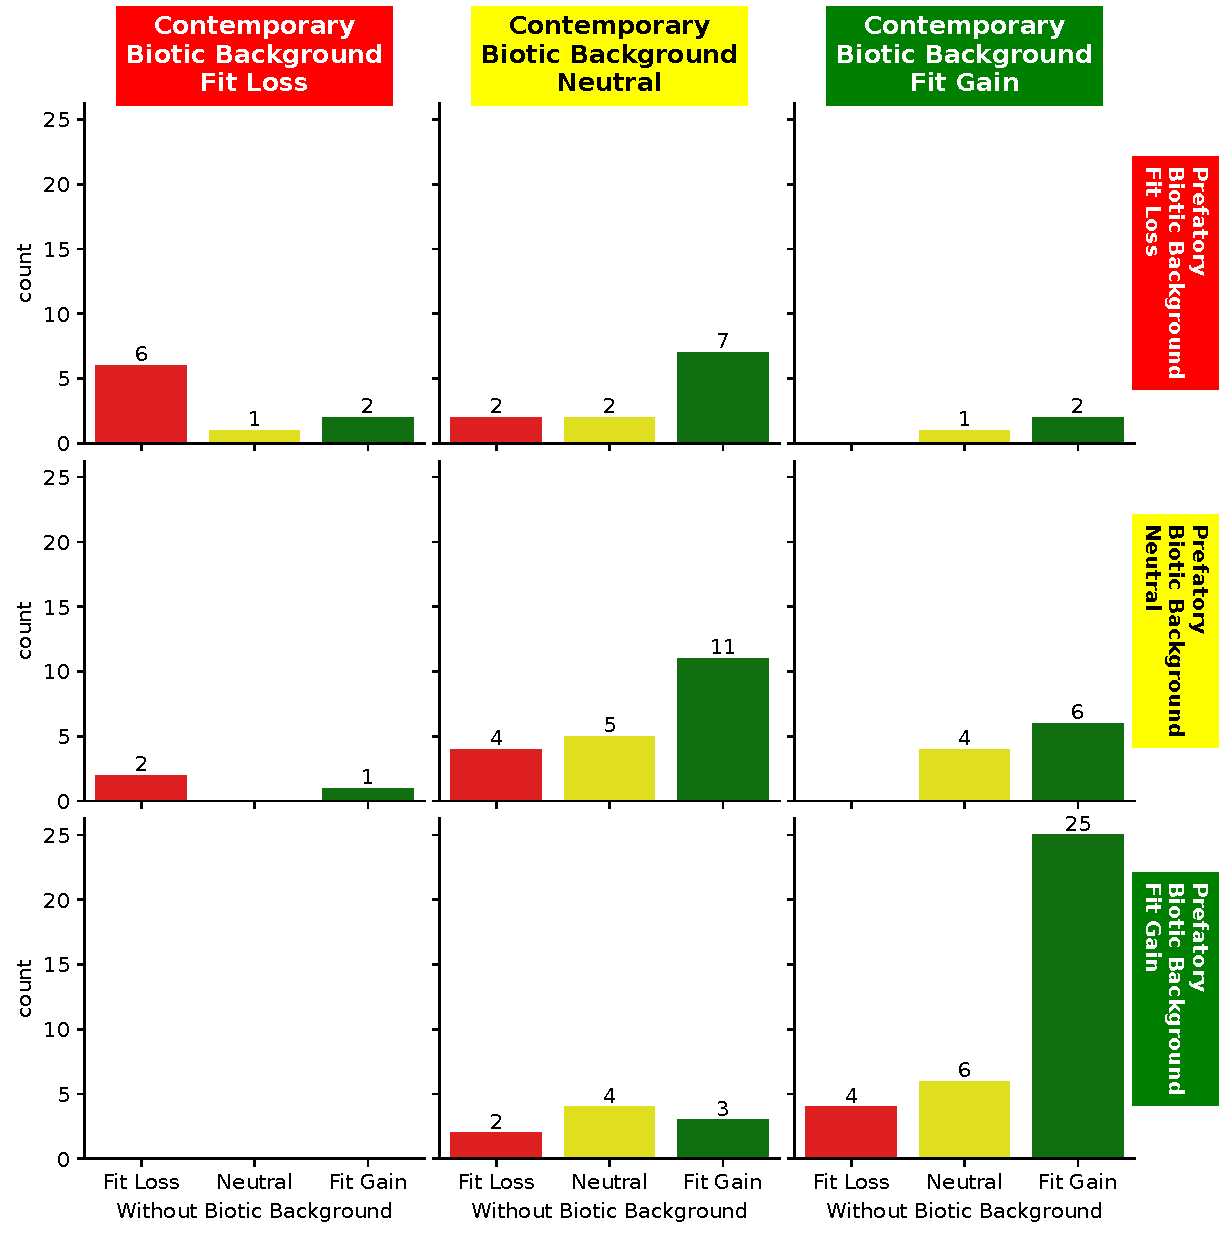
\includegraphics[width=\linewidth]{{submodule/dishtiny/binder/bucket=prq49/a=adaptation_assays+endeavor=16/teeplots/assay-subject=Specimen+col=contemporary-biotic-background+kind=count+row=prefatory-biotic-background+viz=barlabel-catplot+x=without-biotic-background+ext=}}
\caption{Joint distribution of adaptation assay on representative specimen from focal strain over biotic backgrounds, with diversity maintenance during competition.}
\label{fig:outcome_count_joint_distns:specimen_with_dm}
\end{subfigure}%
\hfill%
\begin{subfigure}[t]{0.32\textwidth}
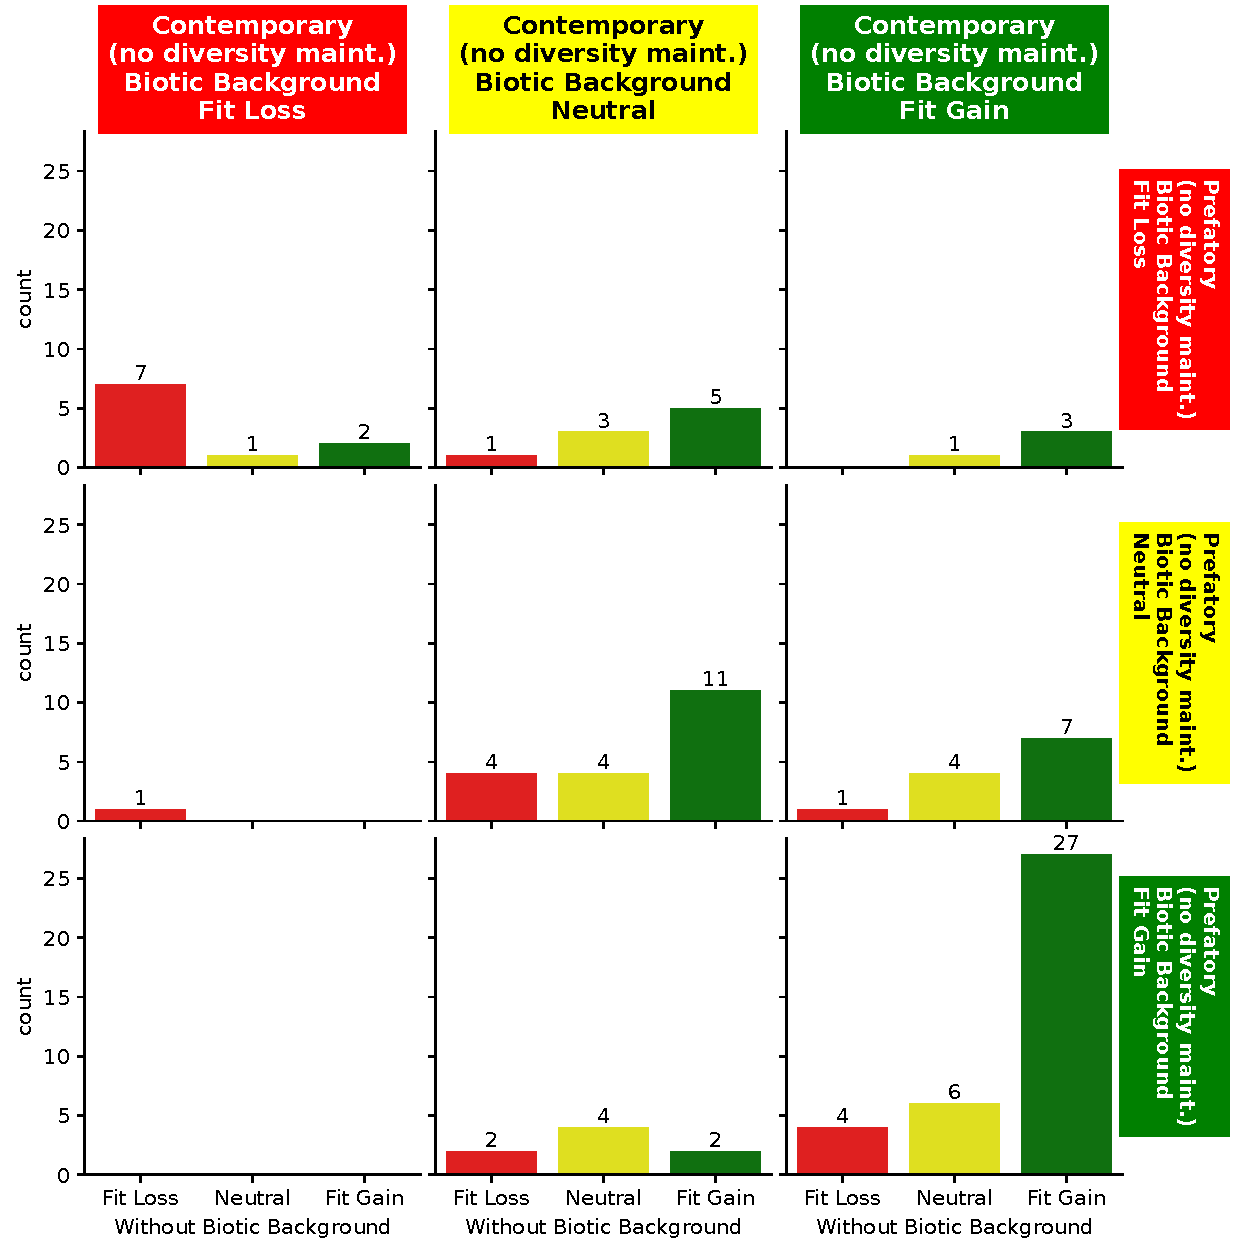
\includegraphics[width=\linewidth]{{submodule/dishtiny/binder/bucket=prq49/a=adaptation_assays+endeavor=16/teeplots/assay-subject=Specimen+col=contemporary-no-diversity-maint-biotic-background+kind=count+row=prefatory-no-diversity-maint-biotic-background+viz=barlabel-catplot+x=without-biotic-background+ext=}}
\caption{Joint distribution of adaptation assay on representative specimen from focal strain over biotic backgrounds, with diversity maintenance disabled during competition.}
\label{fig:outcome_count_joint_distns:specimen_no_dm}
\end{subfigure}%
\hfill%
\begin{subfigure}[t]{0.32\textwidth}
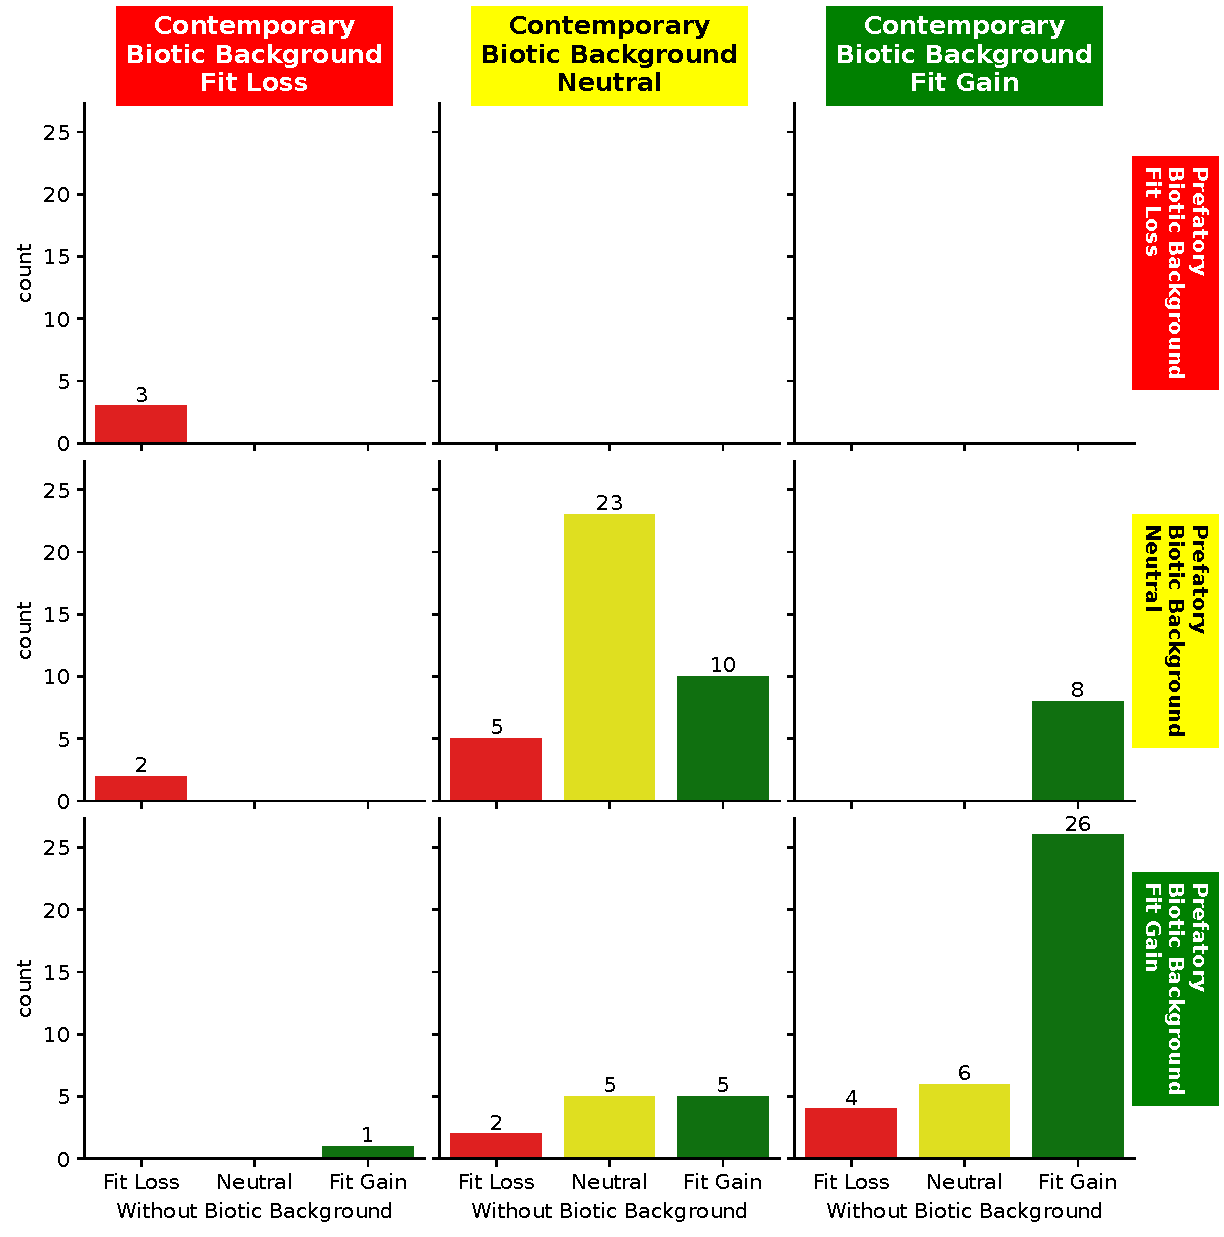
\includegraphics[width=\linewidth]{{submodule/dishtiny/binder/bucket=prq49/a=adaptation_assays+endeavor=16/teeplots/assay-subject=Population+col=contemporary-biotic-background+kind=count+row=prefatory-biotic-background+viz=barlabel-catplot+x=without-biotic-background+ext=}}
\caption{Joint distribution of adaptation assay on focal strain population over biotic backgrounds, with diversity maintenance during competition.}
\label{fig:outcome_count_joint_distns:population}
\end{subfigure}


\caption{
\textbf{Effect of biotic background on adaptation assay outcomes.}
\footnotesize
Joint distribution of adaptation assay outcomes across biotic backgrounds.
For each adaptation assay, three outcomes were possible: significant fitness gain, significant fitness loss, or no significant fitness change (``neutral'').
Significance cutoff $p < 0.005$ was used.
A fitness loss --- color-coded red --- corresponds to winning 2 or fewer competitions out of 20 against the preceding stint's focal strain population.
A fitness gain --- color-coded green --- corresponds to winning 18 or more competitions out of 20 against the preceding stint's focal strain population.
Neutral fitness outcomes are color-coded yellow.
Outcome counts are accumulated over experiments from stint 1 through stint 100.
Counts in each subfigure therefore sum to 100.
Column position in facet grid indicates outcome with contemporary biotic background, row position indicates outcome with prefatory biotic background, and bar color and $x$ position indicates outcome without biotic background.
See Figure \ref{fig:adaptation_assay_cartoon} for explanation of competition biotic backgrounds.
See Figure \ref{fig:with_vs_without_diversity_maintenance} for detail on joint distribution of outcomes with and without diversity maintenance, which were mostly identical.
}
\label{fig:outcome_count_joint_distns}
\end{sidewaysfigure*}


After incorporating the background strain into our measure of fitness, we detected fewer whole-population deleterious outcomes --- only six under contemporary biotic background conditions and only three under prefatory biotic background conditions (Figure \ref{fig:outcome_count_distns}).
To determine whether the presence of the background strain caused the overall reduction in whole-population deleterious outcomes, we performed a control competitions under biotic background conditions, but with the focal strain population substituted for the background strain population (Supplementary Figure \ref{fig:baseline_adaptation_control}).
Under these conditions, nine of the stints where whole-population deleterious outcomes had been detected came up neutral and one, surprisingly, tested significantly adaptive (Supplementary Figure \ref{fig:baseline_fitness_gain_or_loss}).
Dose-dependent fitness effects and/or reduced experimental sensitivity of the biotic background assay appear to play at least a partial role in explaining the reduction of detected whole-population deleterious outcomes.
However, 10 stints still tested significantly deleterious with the control focal strain biotic background in addition to without biotic background.

Four stints do provide strong, direct evidence of a selective effect by the background strain: four whole-population outcomes that were deleterious without biotic background were actually significantly advantageous in the presence of both the prefatory and contemporary background strain populations (Figure \ref{fig:outcome_count_joint_distns:population}).
All four of these stints exhibited whole-population deleterious outcomes under the control focal strain biotic background, indicating that the observed fitness sign change was specifically due to the presence of the background strain (Supplementary Figure \ref{fig:baseline_fitness_gain_or_loss}).

Additionally, two deleterious outcomes without biotic background were detected as significantly adaptive under the prefatory biotic background but were neutral under contemporary biotic background (Figure \ref{fig:outcome_count_joint_distns:population}).
Control focal strain biotic background experiments again suggest that the background strain, specifically, is responsible for this effect (Supplementary Figure \ref{fig:baseline_fitness_gain_or_loss}).

% A further five outcomes were detected as significantly deleterious without biotic background but were not detected as significantly adaptive or deleterious (i.e., neutral) in the presence of both background strain populations (Figure \ref{fig:outcome_count_joint_distns:population}).
We also found one whole-population outcome that was significantly advantageous without biotic background and in the presence of the prefatory background strain population but significantly deleterious in the presence of the contemporary background strain, possibly suggesting a ``arms race''-like evolutionary innovation on the part of the background strain over that stint (Figure \ref{fig:outcome_count_joint_distns:population}).

We still saw three whole-population outcomes that were significantly deleterious under all three conditions (Figure \ref{fig:outcome_count_joint_distns:population}).
These whole-population outcomes were also deleterious under the control focal strain biotic background experiments (Supplementary Figure \ref{fig:baseline_fitness_gain_or_loss}).
Muller's ratchet \citep{andersson1996muller} or maladaptation due to environmental change \citep{brady2019causes} may provide possible explanations, but a definitive answer will require further study.

We also performed fitness assays on individual sampled specimens with both biotic backgrounds.
Out of 100 stints tested, we observed 20 significantly deleterious outcomes without biotic background, 23 significantly deleterious outcomes under prefatory biotic background, and 12 significantly deleterious outcomes under contemporary biotic background (Figure \ref{fig:outcome_count_distns}).
Reciprocally, we observed 57 significantly adaptive outcomes without biotic background, 44 with prefatory biotic background, and 48 with contemporary biotic background (Figure \ref{fig:outcome_count_distns}).
Greater sensitivity of the ``without biotic background'' adaptation assay could account for the counterintuitive detection of more adaptive outcomes under abiotic conditions (i.e., the absence of the background strain).

As before with the population-level adaptation assays, we detected four specimen outcomes that were deleterious without biotic background but significantly advantageous under both tested background strain populations (Figure \ref{fig:outcome_count_joint_distns:specimen_with_dm}).
Additionally, and again as before, two deleterious outcomes without biotic background were detected as significantly adaptive under the prefatory biotic background but neutral under the contemporary biotic background (Figure \ref{fig:outcome_count_joint_distns:specimen_with_dm}).
Control focal strain biotic background experiments confirm that the background strain, specifically, is responsible for these effects (Supplementary Figure \ref{fig:baseline_fitness_gain_or_loss}).

We found no specimen outcomes that were advantageous under the prefatory biotic background but deleterious under the contemporary background.
However, we found three stints with opposite dynamics: specimen outcomes deleterious under prefatory biotic background but advantageous under contemporary biotic background (Figure \ref{fig:outcome_count_joint_distns:specimen_with_dm}), further suggesting coincident, interacting evolutionary innovations along focal and background strain lineages (Figure \ref{fig:outcome_count_joint_distns:specimen_with_dm}).

\begin{figure*}
\centering
\captionsetup[subfigure]{font=footnotesize}
\begin{subfigure}[t]{0.49\textwidth}
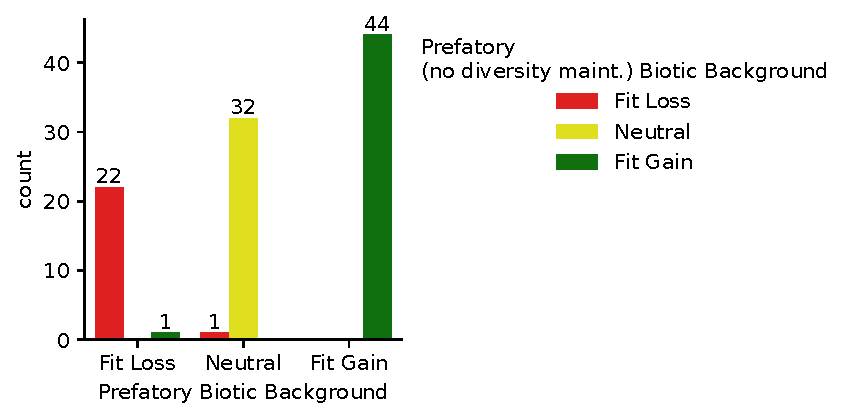
\includegraphics[width=\linewidth]{{submodule/dishtiny/binder/bucket=prq49/a=adaptation_assays+endeavor=16/teeplots/assay-subject=Specimen+hue=prefatory-no-diversity-maint-biotic-background+kind=count+viz=barlabel-catplot+x=prefatory-biotic-background+ext=}}
\caption{prefatory biotic background outcomes with and without diversity maintenance}
\end{subfigure}%
\hfill%
\begin{subfigure}[t]{0.49\textwidth}
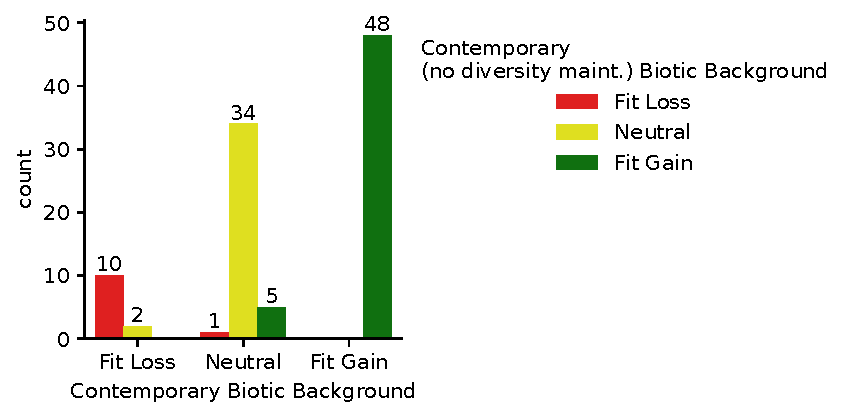
\includegraphics[width=\linewidth]{{submodule/dishtiny/binder/bucket=prq49/a=adaptation_assays+endeavor=16/teeplots/assay-subject=Specimen+hue=contemporary-no-diversity-maint-biotic-background+kind=count+viz=barlabel-catplot+x=contemporary-biotic-background+ext=}}
\caption{contemporary biotic background outcomes with and without diversity maintenance}
\end{subfigure}

\caption{
\textbf{Effect of diversity maintenance on adaptation assays with biotic background.}
\footnotesize
Joint distribution of competition experiments performed under biotic background conditions with diversity maintenance enabled and disabled.
Color coding denotes outcome without diversity maintenance and $x$ position denotes outcome with diversity maintenance.
Note that both plots above show distributions for adaptation assays on representative specimens.
Competition experiments without diversity maintenance were not performed for population-level adaptation.
See Figure \ref{fig:adaptation_assay_cartoon} for explanation of competition biotic backgrounds.
}
\label{fig:with_vs_without_diversity_maintenance}
\end{figure*}


To better characterize the mechanism of fitness effects caused by the background strain, we performed additional competition experiments with sampled specimens in the presence of the background strain population with diversity maintenance disabled.
This allowed us to test whether action of the diversity maintenance mechanism, rather than direct interactions between the focal and background strains, caused the observed fitness effects.
Figure \ref{fig:with_vs_without_diversity_maintenance} compares adaptation assay outcomes with and without diversity maintenance under both the prefatory and contemporary biotic background conditions.
Outcomes were generally similar, and only one sign-change difference was observed: one specimen outcome was beneficial under prefatory biotic background conditions without diversity maintenance but deleterious with diversity maintenance.
Further, as shown in Figure \ref{fig:outcome_count_joint_distns:specimen_no_dm}, we observed near-identical sign-change fitness effects of biotic background as noted above.
So, biotic selective effects cannot be explained as an artifact of activation of the diversity maintenance scheme.

\begin{sidewaysfigure*}
\thisfloatpagestyle{mylandscape}%
\rotatesidewayslabel%
\centering
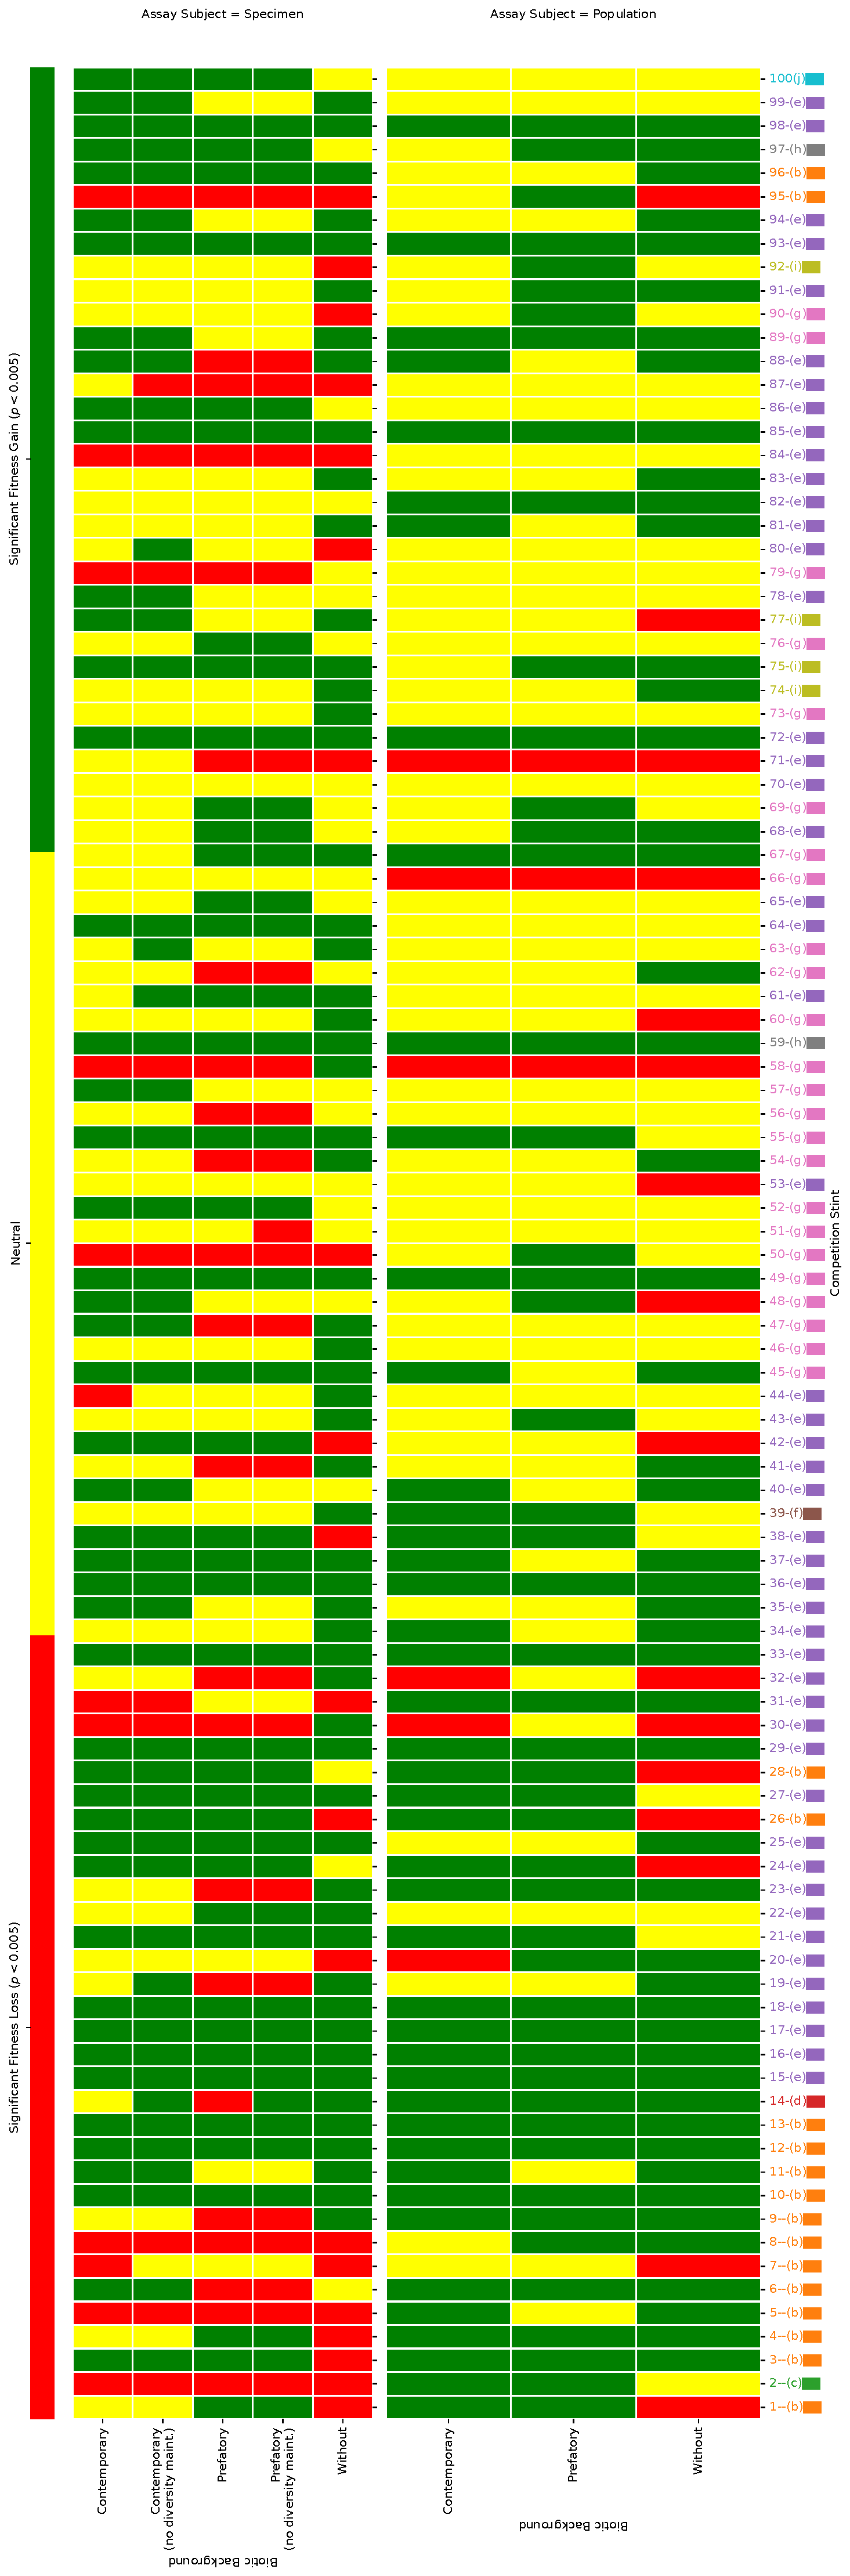
\includegraphics[width=\linewidth]{{submodule/dishtiny/binder/bucket=prq49/a=adaptation_assays+endeavor=16/teeplots/hue=fitness-gain-or-loss+viz=facet-heatmap+x=biotic-background+y=competition-stint+ext=}}

\caption{
\textbf{Adaptation Assay Outcomes.}
\footnotesize
Summary of adaptation assay outcomes for sampled representative specimen (top) and population-level adaptation (bottom).
Color coding and parentheticals of stint labels correspond to qualitative morph codes described in Table \ref{tab:morph_descriptions}.
See Figure \ref{fig:adaptation_assay_cartoon} for explanation of competition biotic backgrounds.
}
\label{fig:fitness_gain_or_loss}
\end{sidewaysfigure*}


Significant increases in fitness occur throughout the evolutionary history of the case study, but not at every stint.
Figure \ref{fig:fitness_gain_or_loss} summarizes the outcome of all adaptation assays stint-by-stint across evolutionary history.
Neutral outcomes appear to occur more frequently at later stints.
This may be indicative of slower evolutionary innovation, but may also result to some extent from simulation of fewer generations during evolutionary stints (Supplementary Figure \ref{fig:simulation}) and during competition experiments (Supplementary Figure \ref{fig:num_updates_elapsed_barplot}) due to slower execution of later genomes.

\begin{sidewaysfigure*}
\centering
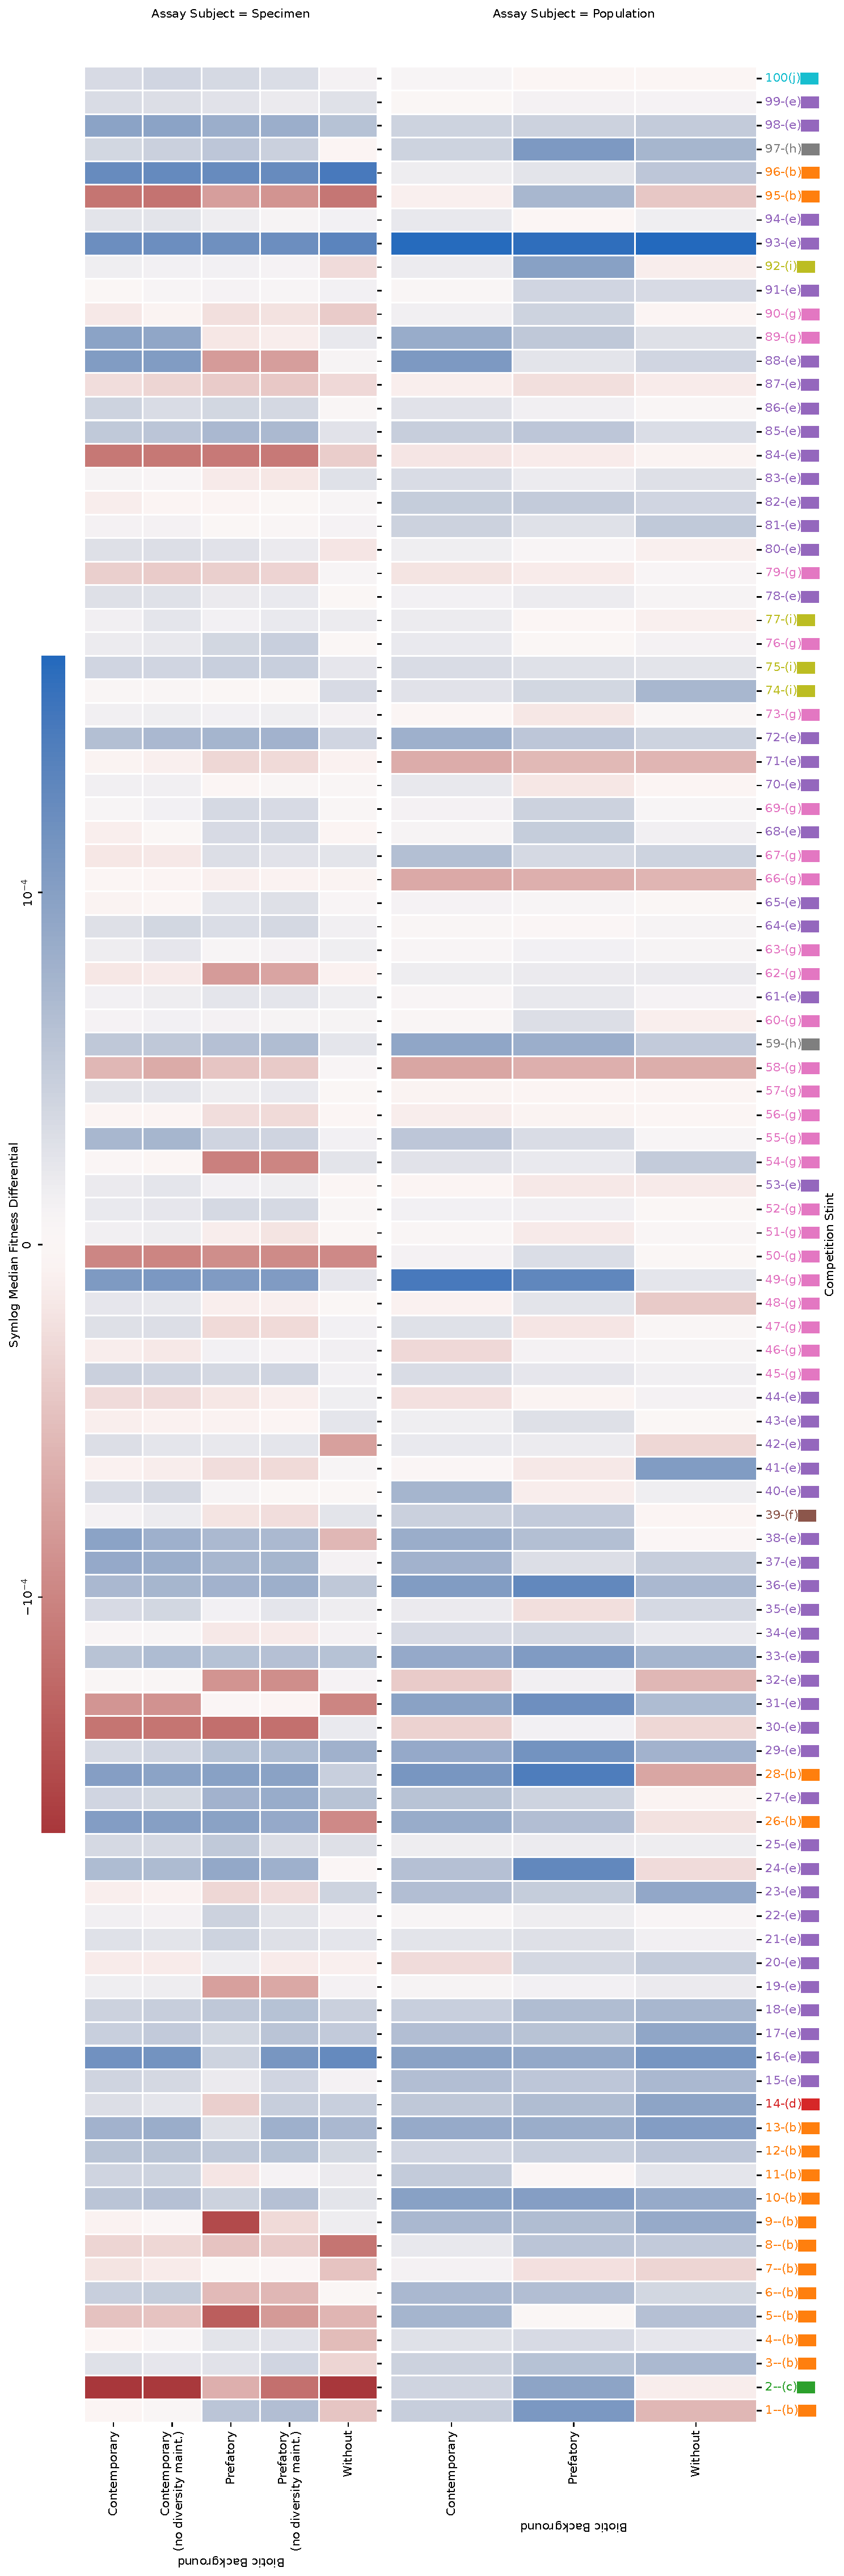
\includegraphics[width=\linewidth]{{submodule/dishtiny/binder/bucket=prq49/a=adaptation_assays+endeavor=16/teeplots/hue=symlog-median-fitness-differential+viz=facet-heatmap+x=biotic-background+y=competition-stint+ext=}}

\caption{
TODO
}
\label{fig:median_fitness_differential_symlog}
\end{sidewaysfigure*}


Figure \ref{fig:median_fitness_differential_symlog} shows the magnitudes of calculated fitness differentials for all adaptation assays.
Fitness differentials during the first 40 stints are generally higher magnitude than later fitness differentials, although a very strong fitness differential occurs at stint 93.
Although the emergence of morphology $d$ was associated with significant increases in fitness in some specimen assays and morphologies $e$ and $g$ were associated with significant increases in fitness across all specimen assays (Figure \ref{fig:fitness_gain_or_loss}), the magnitude of these fitness differentials appears ordinary compared to fitness differentials at other stints (Figure \ref{fig:median_fitness_differential_symlog}).
Supplementary Figure \ref{fig:mean_competition_prevalence} shows mean end-competition prevalence across assays, telling a similar story.

\begin{figure}

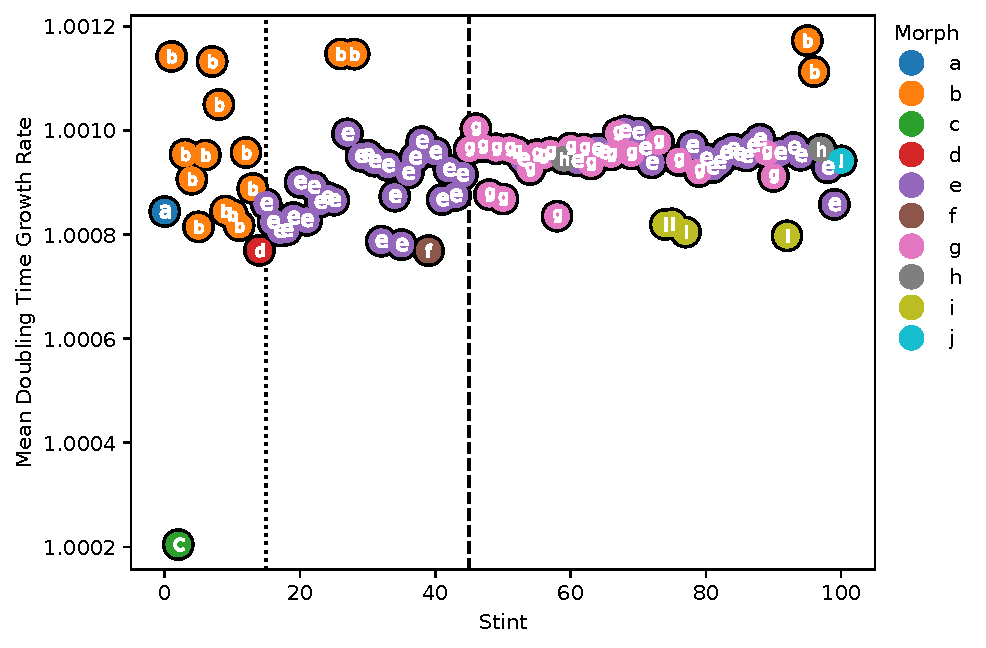
\includegraphics[width=\linewidth]{{plots/fitness/bucket=prq49+cat=morph+endeavor=16+transform=filter-Series-16005+viz=letterscatter-vline+x=stint+y=mean-doubling-time-growth-rate+ext=}}

\caption{Growth rate estimated from doubling time experiments, measuring time for a monoculture to grow from 0.25 maximum population size to 0.5 maximum population size.}
\label{fig:doubling_time}

\end{figure}


In addition to competition assays, we also measured growth rate of specimen strains by tracking doubling time (in updates) when seeded into quarter-full toroidal grids (Figure \ref{fig:doubling_time}).
Morph $b$ exhibited a fast growth rate early on that was never matched by later morphs.
This measure appears to be a poor overall proxy for fitness, highlighting the importance of biotic aspects of the simulation environment (which are not present in the empty space the assayed cells double into).


\subsection{Fitness Complexity}

\begin{figure}

\input{fig/fitness_complexity/critical_fitness_complexity.tex}
% \input{fig/fitness_complexity/interpolated_fitness_complexity.tex}
% \input{fig/fitness_complexity/composite_fitness_complexity.tex}

\caption{ Fitness complexity estimates. Color coding and letters correspond to qualitative morph codes described in Table \ref{tab:morph_descriptions}. 
Dotted vertical line denotes emergence of morph $e$.
Dashed vertical line denotes emergence of morph $g$.
}
\label{fig:fitness_complexity}

\end{figure}

Figure \ref{fig:fitness_complexity:critical_fitness_complexity} plots critical fitness complexity of specimens drawn from across the case study's evolutionary history.

Critical fitness complexity reaches more than 20 under morph $b$, jumps to more than 40 under morph $d$, drops to slightly more than 30 for morph $e$.
Critical fitness complexity reaches a peak of 48 sites around stint 39 then levels out and decreases.
This decrease may in part be due to declining sensitivity of competition experiments due to slower simulation resulting in execution of fewer updates within the fixed-duration jobs (Supplementary Figure \ref{fig:num_updates_elapsed_heatmap}).

Phylogenetic analysis (Figure \ref{fig:phylo_parsimony_tree}) suggests independent origins of the critical fitness complexity in morph $d$ and morph $e$ --- the morph $d$ specimen from stint 14 is more closely related to the morph $b$ specimen from stint 13 than to the morph $e$ specimen from stint 15.
Likewise, specimens of lower complexity morphs $i$ and $b$ that appear past stint 70 appear to have independent evolutionary origins.

% The evolution of morph $g$ is not associated with a clear change in critical fitness complexity.

% Interpolated fitness complexity remains much more steady over the course of evolutionary history, although the certainty of our estimate of interpolated fitness complexity varies greatly.
% Figure \ref{fig:fitness_complexity:interpolated_fitness_complexity} shows this.
% Sometimes we were not able to estimate composite fitness complexity because the phenotype neutral nopout was not truly neutral --- it was significantly less fit than wildtype.

% Figure \ref{fig:fitness_complexity:composite_fitness_complexity} shows composite fitness complexity, the sum of interpolated fitness complexity and critical fitness complexity.
% The highest best estimate of composite fitness complexity was 64 sites at stint 61.
% The highest lower bound estimate of composite fitness complexity was 49 sites at stint 70.

\subsection{Interface Complexity}

\input{lib/dissertationonly.tex}
\begin{figure*}
\dissertationonly{\captionsetup[subfigure]{font=scriptsize}}
\dissertationonly{\captionsetup{font=footnotesize}}
\input{fig/interface_complexity/cardinal_interface_complexity.tex}
\input{fig/interface_complexity/intermessage_interface_complexity.tex}
\input{fig/interface_complexity/intramessage_interface_complexity.tex}
\input{fig/interface_complexity/introspective_interface_complexity.tex}
\input{fig/interface_complexity/extrospective_interface_complexity.tex}
\input{fig/interface_complexity/writable_interface_complexity.tex}

\caption{ Interface complexity estimates. Color coding and letters correspond to qualitative morph codes described in Table \ref{tab:morph_descriptions}.
Dotted vertical line denotes emergence of morph $e$.
Dashed vertical line denotes emergence of morph $g$.}
\label{fig:interface_complexity}
\end{figure*}


Figure \ref{fig:interface_complexity} summarizes cardinal interface complexity, as well as its constituent components, for specimens drawn from across the case study's evolutionary history.

Notably, cardinal interface complexity more than doubles from 6 interactions to 17 interactions coincident with the emergence of morph $e$ (Figure \ref{fig:interface_complexity:cardinal_interface_complexity}).
This is due to simultaneous increases in extrospective state sensing (2 to 9 states; Figure \ref{fig:interface_complexity:extrospective_interface_complexity}), introspective state sensing (1 to 4 states; Figure \ref{fig:interface_complexity:introspective_interface_complexity}), and writable state usage (1 to 2 states; Figure \ref{fig:interface_complexity:writable_interface_complexity}).

The emergence of morph $g$ coincided with an increase in writable state interface complexity from 1 to 3 as shown in Figure \ref{fig:interface_complexity:writable_interface_complexity}.
However, morph $g$ was not associated with other changes in other aspects of cardinal interface complexity.
The greatest observed cardinal interface complexity was 22 interactions at stints 54 and 67.

\subsection{Genome Size}

\begin{figure}
\centering
\begin{subfigure}{0.49\textwidth}
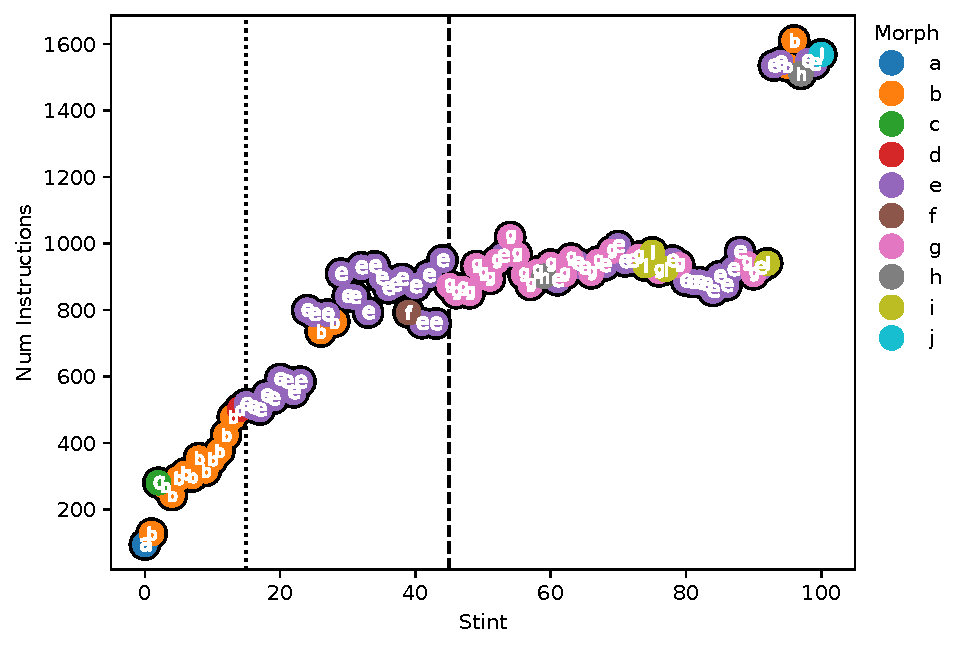
\includegraphics[width=\linewidth]{{submodule/dishtiny/binder/bucket=prq49/a=all_stints_all_series_profiles+endeavor=16/teeplots/bucket=prq49+cat=morph+endeavor=16+transform=filter-Series-16005+viz=letterscatter-vline+x=stint+y=num-instructions+ext=}}
\caption{instruction count}
\label{fig:instruction_count}
\end{subfigure}
\begin{subfigure}{0.49\textwidth}
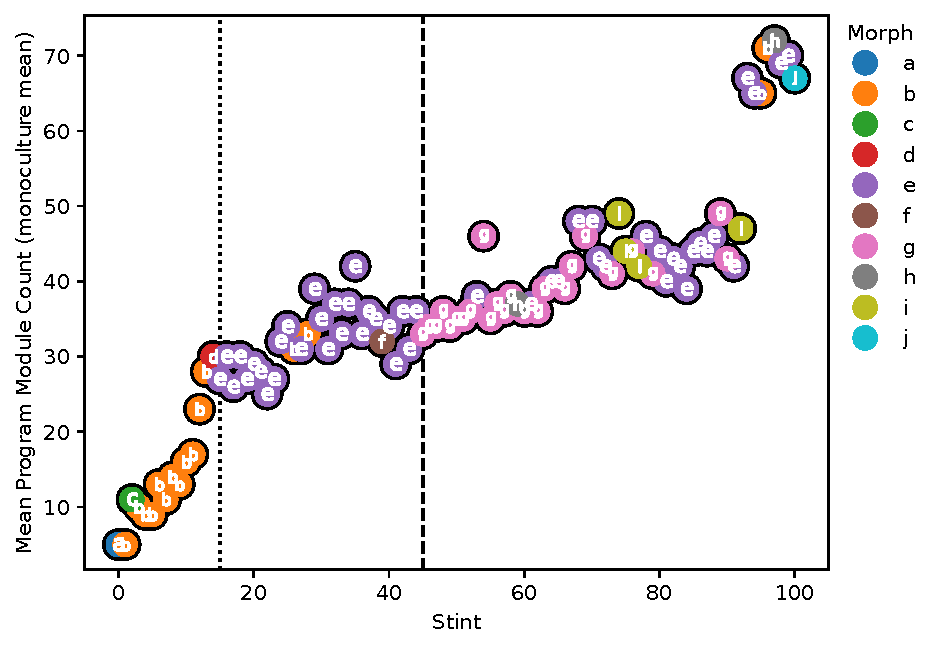
\includegraphics[width=\linewidth]{{submodule/dishtiny/binder/bucket=prq49/a=all_stints_all_series_profiles+endeavor=16/teeplots/bucket=prq49+cat=morph+endeavor=16+transform=filter-Series-16005+viz=letterscatter-vline+x=stint+y=mean-program-module-count-monoculture-mean+ext=}}
\caption{module count}
\label{fig:module_count}
\end{subfigure}
\begin{subfigure}{0.49\textwidth}
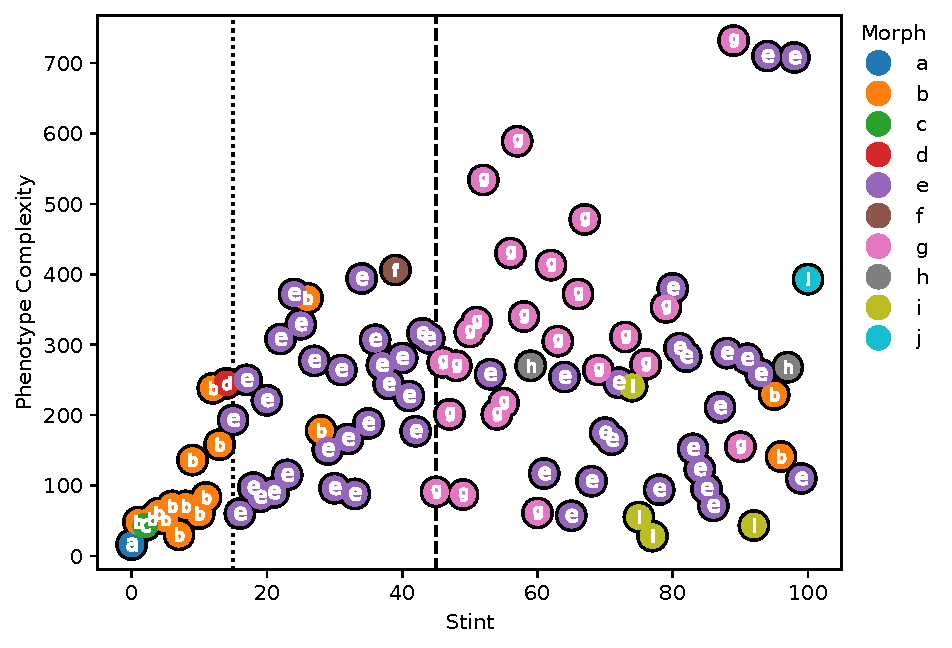
\includegraphics[width=\linewidth]{{plots/phenotype_complexity/bucket=prq49+cat=morph+endeavor=16+transform=filter-Series-16005+viz=letterscatter-vline+x=stint+y=phenotype-complexity+ext=}}
\caption{phenotype complexity}
\label{fig:phenotype_complexity}
\end{subfigure}

\caption{
Genome size of sampled focal strain specimens.
Instruction count is the total number of instructions present in the genome.
Module count is the number of tagged linear GP modules available for activation by signals from the environment, from other agents, or from within an agent.
Phenotype complexity is the number of genome sites that contribute to phenotype, measured as number sites remaining after phenotype-neutral nopout (Section \ref{sec:phenotype_neutral_nopout}).
This measure gives a sense of the number of ``active'' instructions that influence agents' behavior.
Color coding and letters correspond to qualitative morph codes described in Table \ref{tab:morph_descriptions}.
Dotted vertical line denotes emergence of morph $e$.
Dashed vertical line denotes emergence of morph $g$.
}
\label{fig:genome_size}

\end{figure}


Figure \ref{fig:genome_size} shows evolutionary trajectories of three genome size metrics in sampled focal strain specimens.
Instruction count and module count increased from 100 and 5 to around 800 and 30, respectively, between stints 0 and 40.
Within this period at stint 24, instruction count jumped from around 600 to more than 800 and module count jumped by about 5.
This was coincident with detection in our adaptation assays of population-level sign-change mediation of adaptation by the background strain (Figure \ref{fig:fitness_gain_or_loss}).
In sampled specimen fitness assays at stint 24, we detected significant increases in fitness in the presence of the background strain but no significant change in fitness in its absence.

Between stints 40 and 90, module count gradually increased to around 40 while instruction count remained stable.
Then, at stint 93, instruction count jumped to around 1,500 and module count jumped to around 60.
This was coincident with the strong fitness differentials observed at stint 93 (Figure \ref{fig:median_fitness_differential_symlog}).

To better understand the functional effects of changes in genome size, we additionally measured the number of instructions that affected agent phenotype, shown as ``phenotype complexity'' in Figure \ref{fig:phenotype_complexity}.
This measure can be considered akin to a count of ``active'' sites.

Phenotype complexity varied greatly stint to stint.
The median value increased from nearly 0 to around 200 sites between stints 0 and 40.
Between stints 40 and 90, phenotype complexity values ranging from less than 100 to more than 500 were observed.
Morph $g$ specimens appear to show particularly great variance in phenotype complexity.
The first observed morph $g$ specimen at stint 45 exhibited relatively low phenotype complexity of around 100 active sties.
The highest phenotype complexity values of around 700 were measured from three specimens of morphs $e$ and $g$ in the last ten stints.


\section{Discussion}

Throughout the case study lineage, we describe an evolutionary sequence of ten qualitatively distinct multicellular morphologies (Table \ref{tab:morph_descriptions}).
The emergence of some, but not all, of these morphologies coincided with an increase in fitness compared to the preceding population.
Outcomes from the first observed morphology $c$ specimen are significantly deleterious in all contexts.
Likewise, morphology $f$, while advantageous in the absence of the background strain, appeared neutral in its presence (Figure \ref{fig:fitness_gain_or_loss}).
However, the genesis of morphology $e$, and $g$ are associated with significant fitness gain in all contexts (Figure \ref{fig:fitness_gain_or_loss}).
This latter set of novelties might be described as ``innovations,'' which Hochberg et al. define as qualitative novelty associated with an increase in fitness \citep{hochberg2017innovation}.
Interestingly, the magnitude of the fitness differentials associated with the emergence of morphologies $e$, and $g$ do not appear to fall outside the bounds of other stint-to-stint fitness differentials (Figure \ref{fig:median_fitness_differential_symlog}).

The relationship between innovation and complexity also appears to be loosely coupled.
The emergence of morphology $d$ was accompanied by a spike in critical fitness complexity (from 25 sites at stint 13 to 43 sites at stint 14).
However, the emergence of morphology $i$ coincided with a loss of critical fitness complexity (from more than 30 sites to fewer than 10 sites).
The specimen of morph $i$ at stint 77, which phylogenetic analysis suggests may have independent trait origin from the specimen at stint 75, exhibited significant fitness gain across all contexts despite decimation of complexity.

Phylogenetic analysis suggests that morphology $e$ was not a direct descendant of morphology $d$.
So the emergence of morphology $e$ appears to have coincided with a more modest increase in fitness complexity from 25 sites to 31 sites.
Similarly, the emergence of morphology $g$ with 42 critical sites at stint 45 coincided with a relatively modest increase in fitness complexity from 39 critical sites at stint 44.

We also see evidence that increases in complexity do not imply qualitative novelty in morphology.
In Figure \ref{fig:fitness_complexity:critical_fitness_complexity}, we can also observe notable increases in critical fitness complexity that did not coincide with apparent morphological innovation.
For example, fitness complexity jumped from 11 sites at stint 11 to 27 sites at stint 12 while morphology $b$ was retained.
In addition, a more gradual increase in fitness complexity was observed from 27 sites at stint 16 to 46 sites at stint 36 all with consistent morphology $e$.

Finally, we also observed disjointedness between alternate measures of functional complexity.
Notably, critical fitness complexity increased by 18 sites with the emergence of morph $d$ but interface complexity increased only marginally.
Subsequently observed morph $e$ had nearly triple the interface complexity of morph $d$ (6 interactions vs. 17 interactions) but had 12 sites lower critical fitness complexity.
In addition, the gradual increase in critical fitness complexity between stint 15 and 36 under moprhology $e$ is not accompanied by a clear change in interface complexity (Figures \ref{fig:interface_complexity:cardinal_interface_complexity} and \ref{fig:fitness_complexity:critical_fitness_complexity}).
These apparent inconsistencies between metrics for functional complexity evidence the multidimensionality of this idea and underscore well-known difficulties in attempts to describe and quantify it \citep{bottcher2018molecules}.


\section{Conclusion}

Complexity and novelty are not inevitable outcomes of Darwinian evolution \citep{stanley2017open}.
Instead, how and why some lineages within some model systems evolve complexity and novelty merits explanation.
In this regard, efforts to develop substrates and conditions sufficient to observe meaningful evolution of complexity and novelty play a crucial role in assessing the sufficiency of theory.
% Additionally, subsequent availability of complexity and novelty potential within experimental substrates enables work to test and refine theory.
The artificial life research community has a rich track record in such work.

The case study reported here tracks a lineage over two phenotypic innovations and several-fold increases in complexity.
DISHTINY relaxes common simulation constraints \citep{goldsby2012task, goldsby2014evolutionary}, enabling broad genetic determination of multicellular life history and allowing for unconstrained cellular interactions between multicellular bodies.
As such, this case study opens a concrete window into evolutionary origins of complexity and novelty under regimes of strong biotic interactions.

Our case study suggests a loose coupling between novelty, complexity, and adaptation.
We observe instances where novelty coincides with adaptation and instances where it does not.
We observe instances where increases in complexity coincide with adaptation and where decreases in complexity coincide with adaptation.
We observe instances where innovation coincides with spikes in complexity and instances where it does not.
We even observe substantial divergences between metrics measuring different aspects of functional complexity.
For example, the specimen sampled at stint 15 had nearly triple the interface complexity of the specimen sampled at stint 14 but lower critical fitness complexity.

Loose coupling between the conceptual threads of novelty, complexity, and adaptation in this case study highlights the importance of considering these factors independently when developing theory around open-ended evolution --- inherent coupling cannot be assumed.

Our observation of significant selective effects by the background strain suggests that it may serve a crucial role in understanding the focal strain.
Future work should characterize trajectories of adaptation, novelty, and complexity in this background strain.
Additionally, success of the biotic background in fleshing out our adaptation assays suggests that complexity measures could be improved through similar incorporation of the biotic background.
It would be particularly interesting to measure the contribution of the background strain to complexity as the difference between complexity statistics with and without the biotic background.
To more systematically test the role of biotic selection on facilitating evolution of complexity, future experiments might test for differences in the rate of high-complexity evolutionary outcomes between evolution experiments with and without long-term coexistence between lineages (i.e., with diversity maintenance mechanisms enabled versus disabled).

This case study highlights the potential usefulness of toolbox-based approaches to analyzing open-ended evolution systems in which an array of analyses are performed to distinguish disparate dimensions of open-endedness \citep{dolson2019modes}.
Our findings underscore, in particular, the critical role of biotic context in such analyses.
In future work, we are interested in further extending this toolbox.
One priority will be estimating epistatic contributions to fitness without resorting to all-pairs knockouts or other even more extensive assays \citep{moreno2024methods}.
Such methodology will be crucial for systems where fitness is implicit and expensive to measure.


% In future work, we are interested in developing statistical methodology to estimate without .


% This
% Future work exploring open-endedness should continue along the lines of the MODES framework , building a broad analytical toolbox that can distinguish disparate dimensions of open-endedness.

% Continuing the work of MODES to broaden a toolbox rather than focus in on a single metric.

% Serves as a trial balloon for future, more systematic exploration of the relationship between novelty, complexity, and adaptation.

% For example, if that only activated in response to the other lineage then couldn't detect that

% Especially in systems where fitness is implicit it's costly or impractical to do comprehensive analyses.
% We need to continue develop methodology to statisticaly sample

% Problem also that fitness depends on conditions, so there may be problems replicating conditions of evolution environment (presence of mutation, presence of other strains).
% Real-time proof-of-concept but requires more thought about methodology to control for the slowing of evolutionary pace.


% We use the idea of in addition to existing ideas about sequence complexity.
% Interface complexity the richness of interactions between an agent and its environment.
% 8 After all, the central concept of adaptation—``the design or suitability of an object for a particular
% function'' (Gould 2002, p. 117)—directly refers to functionality. A few examples of those taking
% biological functionality as integral to biological complexity include Bronowski (1970), Wicken (1979),
% Dawkins (1986), Kampis and Csa´nyi (1987), Carroll (2001), Adami (2002) \citep{korb2011evolution}

% The question of the relation between sequence complexity and functional complexity is.
% Sequence complexity is defined in terms of entropy of , but in a practical sense it can be approximated by looking at critical fitness complexity.

% a novel innovation is accompanied by a decrease in sequence/critical fitness complexity but an increase in interface complexity.

% Already known in Avida, where sequence/critical fitness complexity would decrease after a innovation as became more adapted

% Surprisingly, the novelty wasn't accompanied by out-of-the ordinary fitness differential.

% However, we present a case study where

% If $d$ is a member of another lineage, then composite fitness complexity didn't increase greatly even though interface complexity more than doubled.

% A second novelty occurs without a clear signal with respect to sequence/fitness complexity or interface complexity.

% Methodology to quantify is particularly critical.
% One area of interest is understanding the functional complexity of .
% Phenotype complexity, Interface complexity and statistical methodololgy to sample stuff.
% We advance proposed methodology by dolson et al with respect to identifying

% We look at a case study to see how these complexity metrics change over an evolutionary history with qualitative moprhological innovations.



\section*{Author Contributions}

\textbf{Conceptualization}: M.A.M., C.A.O. \\
\textbf{Methodology}: M.A.M. \\
\textbf{Software}: M.A.M., S.R.P. \\
\textbf{Writing}: M.A.M. (lead), S.R.P. (supporting contributions) \\
\textbf{Supervision}: C.A.O.

\section*{Competing Interests}

The authors declare no competing interests.

\section*{Data Availability}

All data is available via the Open Science Framework at \url{https://osf.io/prq49} \citep{Moreno_Rodriguez_Papa_2022}.

\section*{Code Availability}

Core DISHTINY code is available under a MIT License at \url{https://github.com/mmore500/dishtiny} \citep{moreno_2025_16990564}.
Code specific to this manuscript is available under a MIT License at \url{https://github.com/mmore500/oee4} \citep{matthew_andres_moreno_2024_16990558}.

\section*{Acknowledgements}

M.A.M. and S.R.J. completed substantial portions of this work while affiliated with the BEACON Center at Michigan State University.

Thanks to members of the DEVOLAB, in particular Katherine Perry for help implementing DISHTINY visualizations.

This research was supported in part by NSF grants DEB-1655715 and DBI-0939454 as well as by Michigan State University through the computational resources provided by the Institute for Cyber-Enabled Research.
This material is based upon work supported by the National Science Foundation Graduate Research Fellowship under Grant No. DGE-1424871.
Any opinions, findings, and conclusions or recommendations expressed in this material are those of the author(s) and do not necessarily reflect the views of the National Science Foundation.

This material is based upon work supported by the Eric and Wendy Schmidt AI in Science Postdoctoral Fellowship, a Schmidt Sciences program.

This material is based upon work supported by the U.S. Department of Energy, Office of Science, Office of Advanced Scientific Computing Research (ASCR), under Award Number DE-SC0025634.
This report was prepared as an account of work sponsored by an agency of the United States Government.
Neither the United States Government nor any agency thereof, nor any of their employees, makes any warranty, express or implied, or assumes any legal liability or responsibility for the accuracy, completeness, or usefulness of any information, apparatus, product, or process disclosed, or represents that its use would not infringe privately owned rights.
Reference herein to any specific commercial product, process, or service by trade name, trademark, manufacturer, or otherwise does not necessarily constitute or imply its endorsement, recommendation, or favoring by the United States Government or any agency thereof.
The views and opinions of authors expressed herein do not necessarily state or reflect those of the United States Government or any agency thereof.


\footnotesize
\bibliographystyle{apalike}
\bibliography{bibl} % replace by the name of your .bib file

\clearpage
\newpage

\appendix

\clearpage
\onecolumn

\vspace*{\fill}
{\Huge
Supplement for ``Case Study of Novelty, Complexity, and Adaptation in a Multicellular System'' by Matthew Andres Moreno, Santiago Rodriguez Papa, and Charles Ofria
in OEE4: The Fourth Workshop on Open-Ended Evolution}
\vspace*{\fill}

\clearpage

\setcounter{secnumdepth}{2}

% \pragmaonce

% adapted from https://www.overleaf.com/learn/latex/Commands
\providecommand{\dissertationelse}[2]{%
% adapted from https://tex.stackexchange.com/a/33577
\ifdefined\DISSERTATION
#1
\else
#2
\fi
}


\newcommand{\tinyurl}[1]{\dissertationelse{\fontsize{8}{8}\selectfont}{\tiny}\url{#1}}

\newcommand{\morphcode}[1]{ \raisebox{-0.8em}{\color[HTML]{FFFFFF} \large \textbf{#1} }}

% \begin{table*}
\begin{longtable}[]{ccp{2.5cm} p{2.5cm} p{2.5cm} p{2.5cm} p{2.5cm}}
% \begin{tabular}{ccl}
\caption{Qualitative morph categorization of representative specimens sampled across evolutionary stints.
Video links provide an time-lapse animation of each specimen's morphology when grown in monoculture.
Web viewer URLs link to an in-browser simulation of each genome or population.
Human Readable genome link will download the corresponding genome as an annotated JSON file.} \label{tab:morph_by_stint} \\
\multicolumn{1}{l}{\textbf{Stint}}               & \textbf{Morph} & \textbf{Monoculture Video Link} & \textbf{Monoculture Web Viewer Link} & \textbf{Population Web Viewer Link} & \textbf{Human Readable Genome Link} \\
\endfirsthead
\caption*{\tablename{} \thetable{} (cont'd)} \\
\multicolumn{1}{l}{\textbf{Stint}}               & \textbf{Morph} & \textbf{Monoculture Video Link} & \textbf{Monoculture Web Viewer Link} & \textbf{Population Web Viewer Link} & \textbf{Human Readable Genome Link} \\
\endhead
0 & \cellcolor[HTML]{4C72B0}{\morphcode{a}} & \tinyurl{https://hopth.ru/21/b=prq49+s=16005+t=0+v=video+w=specimen} & \tinyurl{https://hopth.ru/21/b=prq49+s=16005+t=0+v=simulation+w=specimen} & \tinyurl{https://hopth.ru/21/b=prq49+s=16005+t=0+v=simulation+w=population} & \tinyurl{https://hopth.ru/21/b=prq49+s=16005+t=0+v=text+w=specimen} & \\
1 & \cellcolor[HTML]{DD8452}{\morphcode{b} } & \tinyurl{https://hopth.ru/21/b=prq49+s=16005+t=1+v=video+w=specimen} & \tinyurl{https://hopth.ru/21/b=prq49+s=16005+t=1+v=simulation+w=specimen} & \tinyurl{https://hopth.ru/21/b=prq49+s=16005+t=1+v=simulation+w=population} & \tinyurl{https://hopth.ru/21/b=prq49+s=16005+t=1+v=text+w=specimen} \\
2 & \cellcolor[HTML]{55A868}{\morphcode{c} } & \tinyurl{https://hopth.ru/21/b=prq49+s=16005+t=2+v=video+w=specimen} & \tinyurl{https://hopth.ru/21/b=prq49+s=16005+t=2+v=simulation+w=specimen} & \tinyurl{https://hopth.ru/21/b=prq49+s=16005+t=2+v=simulation+w=population} & \tinyurl{https://hopth.ru/21/b=prq49+s=16005+t=2+v=text+w=specimen} \\
3 & \cellcolor[HTML]{DD8452}{\morphcode{b} } & \tinyurl{https://hopth.ru/21/b=prq49+s=16005+t=3+v=video+w=specimen} & \tinyurl{https://hopth.ru/21/b=prq49+s=16005+t=3+v=simulation+w=specimen} & \tinyurl{https://hopth.ru/21/b=prq49+s=16005+t=3+v=simulation+w=population} & \tinyurl{https://hopth.ru/21/b=prq49+s=16005+t=3+v=text+w=specimen} \\
4 & \cellcolor[HTML]{DD8452}{\morphcode{b} } & \tinyurl{https://hopth.ru/21/b=prq49+s=16005+t=4+v=video+w=specimen} & \tinyurl{https://hopth.ru/21/b=prq49+s=16005+t=4+v=simulation+w=specimen} & \tinyurl{https://hopth.ru/21/b=prq49+s=16005+t=4+v=simulation+w=population} & \tinyurl{https://hopth.ru/21/b=prq49+s=16005+t=4+v=text+w=specimen} \\
5 & \cellcolor[HTML]{DD8452}{\morphcode{b} } & \tinyurl{https://hopth.ru/21/b=prq49+s=16005+t=5+v=video+w=specimen} & \tinyurl{https://hopth.ru/21/b=prq49+s=16005+t=5+v=simulation+w=specimen} & \tinyurl{https://hopth.ru/21/b=prq49+s=16005+t=5+v=simulation+w=population} & \tinyurl{https://hopth.ru/21/b=prq49+s=16005+t=5+v=text+w=specimen} \\
6 & \cellcolor[HTML]{DD8452}{\morphcode{b} } & \tinyurl{https://hopth.ru/21/b=prq49+s=16005+t=6+v=video+w=specimen} & \tinyurl{https://hopth.ru/21/b=prq49+s=16005+t=6+v=simulation+w=specimen} & \tinyurl{https://hopth.ru/21/b=prq49+s=16005+t=6+v=simulation+w=population} & \tinyurl{https://hopth.ru/21/b=prq49+s=16005+t=6+v=text+w=specimen} \\
7 & \cellcolor[HTML]{DD8452}{\morphcode{b} } & \tinyurl{https://hopth.ru/21/b=prq49+s=16005+t=7+v=video+w=specimen} & \tinyurl{https://hopth.ru/21/b=prq49+s=16005+t=7+v=simulation+w=specimen} & \tinyurl{https://hopth.ru/21/b=prq49+s=16005+t=7+v=simulation+w=population} & \tinyurl{https://hopth.ru/21/b=prq49+s=16005+t=7+v=text+w=specimen} \\
8 & \cellcolor[HTML]{DD8452}{\morphcode{b} } & \tinyurl{https://hopth.ru/21/b=prq49+s=16005+t=8+v=video+w=specimen} & \tinyurl{https://hopth.ru/21/b=prq49+s=16005+t=8+v=simulation+w=specimen} & \tinyurl{https://hopth.ru/21/b=prq49+s=16005+t=8+v=simulation+w=population} & \tinyurl{https://hopth.ru/21/b=prq49+s=16005+t=8+v=text+w=specimen} \\
9 & \cellcolor[HTML]{DD8452}{\morphcode{b} } & \tinyurl{https://hopth.ru/21/b=prq49+s=16005+t=9+v=video+w=specimen} & \tinyurl{https://hopth.ru/21/b=prq49+s=16005+t=9+v=simulation+w=specimen} & \tinyurl{https://hopth.ru/21/b=prq49+s=16005+t=9+v=simulation+w=population} & \tinyurl{https://hopth.ru/21/b=prq49+s=16005+t=9+v=text+w=specimen} \\
10 & \cellcolor[HTML]{DD8452}{\morphcode{b} } & \tinyurl{https://hopth.ru/21/b=prq49+s=16005+t=10+v=video+w=specimen} & \tinyurl{https://hopth.ru/21/b=prq49+s=16005+t=10+v=simulation+w=specimen} & \tinyurl{https://hopth.ru/21/b=prq49+s=16005+t=10+v=simulation+w=population} & \tinyurl{https://hopth.ru/21/b=prq49+s=16005+t=10+v=text+w=specimen} \\
11 & \cellcolor[HTML]{DD8452}{\morphcode{b} } & \tinyurl{https://hopth.ru/21/b=prq49+s=16005+t=11+v=video+w=specimen} & \tinyurl{https://hopth.ru/21/b=prq49+s=16005+t=11+v=simulation+w=specimen} & \tinyurl{https://hopth.ru/21/b=prq49+s=16005+t=11+v=simulation+w=population} & \tinyurl{https://hopth.ru/21/b=prq49+s=16005+t=11+v=text+w=specimen} \\
12 & \cellcolor[HTML]{DD8452}{\morphcode{b} } & \tinyurl{https://hopth.ru/21/b=prq49+s=16005+t=12+v=video+w=specimen} & \tinyurl{https://hopth.ru/21/b=prq49+s=16005+t=12+v=simulation+w=specimen} & \tinyurl{https://hopth.ru/21/b=prq49+s=16005+t=12+v=simulation+w=population} & \tinyurl{https://hopth.ru/21/b=prq49+s=16005+t=12+v=text+w=specimen} \\
13 & \cellcolor[HTML]{DD8452}{\morphcode{b} } & \tinyurl{https://hopth.ru/21/b=prq49+s=16005+t=13+v=video+w=specimen} & \tinyurl{https://hopth.ru/21/b=prq49+s=16005+t=13+v=simulation+w=specimen} & \tinyurl{https://hopth.ru/21/b=prq49+s=16005+t=13+v=simulation+w=population} & \tinyurl{https://hopth.ru/21/b=prq49+s=16005+t=13+v=text+w=specimen} \\
14 & \cellcolor[HTML]{C44E52}{\morphcode{d} } & \tinyurl{https://hopth.ru/21/b=prq49+s=16005+t=14+v=video+w=specimen} & \tinyurl{https://hopth.ru/21/b=prq49+s=16005+t=14+v=simulation+w=specimen} & \tinyurl{https://hopth.ru/21/b=prq49+s=16005+t=14+v=simulation+w=population} & \tinyurl{https://hopth.ru/21/b=prq49+s=16005+t=14+v=text+w=specimen} \\
15 & \cellcolor[HTML]{8172B3}{\morphcode{e} } & \tinyurl{https://hopth.ru/21/b=prq49+s=16005+t=15+v=video+w=specimen} & \tinyurl{https://hopth.ru/21/b=prq49+s=16005+t=15+v=simulation+w=specimen} & \tinyurl{https://hopth.ru/21/b=prq49+s=16005+t=15+v=simulation+w=population} & \tinyurl{https://hopth.ru/21/b=prq49+s=16005+t=15+v=text+w=specimen} \\
16 & \cellcolor[HTML]{8172B3}{\morphcode{e} } & \tinyurl{https://hopth.ru/21/b=prq49+s=16005+t=16+v=video+w=specimen} & \tinyurl{https://hopth.ru/21/b=prq49+s=16005+t=16+v=simulation+w=specimen} & \tinyurl{https://hopth.ru/21/b=prq49+s=16005+t=16+v=simulation+w=population} & \tinyurl{https://hopth.ru/21/b=prq49+s=16005+t=16+v=text+w=specimen} \\
17 & \cellcolor[HTML]{8172B3}{\morphcode{e} } & \tinyurl{https://hopth.ru/21/b=prq49+s=16005+t=17+v=video+w=specimen} & \tinyurl{https://hopth.ru/21/b=prq49+s=16005+t=17+v=simulation+w=specimen} & \tinyurl{https://hopth.ru/21/b=prq49+s=16005+t=17+v=simulation+w=population} & \tinyurl{https://hopth.ru/21/b=prq49+s=16005+t=17+v=text+w=specimen} \\
18 & \cellcolor[HTML]{8172B3}{\morphcode{e} } & \tinyurl{https://hopth.ru/21/b=prq49+s=16005+t=18+v=video+w=specimen} & \tinyurl{https://hopth.ru/21/b=prq49+s=16005+t=18+v=simulation+w=specimen} & \tinyurl{https://hopth.ru/21/b=prq49+s=16005+t=18+v=simulation+w=population} & \tinyurl{https://hopth.ru/21/b=prq49+s=16005+t=18+v=text+w=specimen} \\
19 & \cellcolor[HTML]{8172B3}{\morphcode{e} } & \tinyurl{https://hopth.ru/21/b=prq49+s=16005+t=19+v=video+w=specimen} & \tinyurl{https://hopth.ru/21/b=prq49+s=16005+t=19+v=simulation+w=specimen} & \tinyurl{https://hopth.ru/21/b=prq49+s=16005+t=19+v=simulation+w=population} & \tinyurl{https://hopth.ru/21/b=prq49+s=16005+t=19+v=text+w=specimen} \\
20 & \cellcolor[HTML]{8172B3}{\morphcode{e} } & \tinyurl{https://hopth.ru/21/b=prq49+s=16005+t=20+v=video+w=specimen} & \tinyurl{https://hopth.ru/21/b=prq49+s=16005+t=20+v=simulation+w=specimen} & \tinyurl{https://hopth.ru/21/b=prq49+s=16005+t=20+v=simulation+w=population} & \tinyurl{https://hopth.ru/21/b=prq49+s=16005+t=20+v=text+w=specimen} \\
21 & \cellcolor[HTML]{8172B3}{\morphcode{e} } & \tinyurl{https://hopth.ru/21/b=prq49+s=16005+t=21+v=video+w=specimen} & \tinyurl{https://hopth.ru/21/b=prq49+s=16005+t=21+v=simulation+w=specimen} & \tinyurl{https://hopth.ru/21/b=prq49+s=16005+t=21+v=simulation+w=population} & \tinyurl{https://hopth.ru/21/b=prq49+s=16005+t=21+v=text+w=specimen} \\
22 & \cellcolor[HTML]{8172B3}{\morphcode{e} } & \tinyurl{https://hopth.ru/21/b=prq49+s=16005+t=22+v=video+w=specimen} & \tinyurl{https://hopth.ru/21/b=prq49+s=16005+t=22+v=simulation+w=specimen} & \tinyurl{https://hopth.ru/21/b=prq49+s=16005+t=22+v=simulation+w=population} & \tinyurl{https://hopth.ru/21/b=prq49+s=16005+t=22+v=text+w=specimen} \\
23 & \cellcolor[HTML]{8172B3}{\morphcode{e} } & \tinyurl{https://hopth.ru/21/b=prq49+s=16005+t=23+v=video+w=specimen} & \tinyurl{https://hopth.ru/21/b=prq49+s=16005+t=23+v=simulation+w=specimen} & \tinyurl{https://hopth.ru/21/b=prq49+s=16005+t=23+v=simulation+w=population} & \tinyurl{https://hopth.ru/21/b=prq49+s=16005+t=23+v=text+w=specimen} \\
24 & \cellcolor[HTML]{8172B3}{\morphcode{e} } & \tinyurl{https://hopth.ru/21/b=prq49+s=16005+t=24+v=video+w=specimen} & \tinyurl{https://hopth.ru/21/b=prq49+s=16005+t=24+v=simulation+w=specimen} & \tinyurl{https://hopth.ru/21/b=prq49+s=16005+t=24+v=simulation+w=population} & \tinyurl{https://hopth.ru/21/b=prq49+s=16005+t=24+v=text+w=specimen} \\
25 & \cellcolor[HTML]{8172B3}{\morphcode{e} } & \tinyurl{https://hopth.ru/21/b=prq49+s=16005+t=25+v=video+w=specimen} & \tinyurl{https://hopth.ru/21/b=prq49+s=16005+t=25+v=simulation+w=specimen} & \tinyurl{https://hopth.ru/21/b=prq49+s=16005+t=25+v=simulation+w=population} & \tinyurl{https://hopth.ru/21/b=prq49+s=16005+t=25+v=text+w=specimen} \\
26 & \cellcolor[HTML]{DD8452}{\morphcode{b} } & \tinyurl{https://hopth.ru/21/b=prq49+s=16005+t=26+v=video+w=specimen} & \tinyurl{https://hopth.ru/21/b=prq49+s=16005+t=26+v=simulation+w=specimen} & \tinyurl{https://hopth.ru/21/b=prq49+s=16005+t=26+v=simulation+w=population} & \tinyurl{https://hopth.ru/21/b=prq49+s=16005+t=26+v=text+w=specimen} \\
27 & \cellcolor[HTML]{8172B3}{\morphcode{e} } & \tinyurl{https://hopth.ru/21/b=prq49+s=16005+t=27+v=video+w=specimen} & \tinyurl{https://hopth.ru/21/b=prq49+s=16005+t=27+v=simulation+w=specimen} & \tinyurl{https://hopth.ru/21/b=prq49+s=16005+t=27+v=simulation+w=population} & \tinyurl{https://hopth.ru/21/b=prq49+s=16005+t=27+v=text+w=specimen} \\
28 & \cellcolor[HTML]{DD8452}{\morphcode{b} } & \tinyurl{https://hopth.ru/21/b=prq49+s=16005+t=28+v=video+w=specimen} & \tinyurl{https://hopth.ru/21/b=prq49+s=16005+t=28+v=simulation+w=specimen} & \tinyurl{https://hopth.ru/21/b=prq49+s=16005+t=28+v=simulation+w=population} & \tinyurl{https://hopth.ru/21/b=prq49+s=16005+t=28+v=text+w=specimen} \\
29 & \cellcolor[HTML]{8172B3}{\morphcode{e} } & \tinyurl{https://hopth.ru/21/b=prq49+s=16005+t=29+v=video+w=specimen} & \tinyurl{https://hopth.ru/21/b=prq49+s=16005+t=29+v=simulation+w=specimen} & \tinyurl{https://hopth.ru/21/b=prq49+s=16005+t=29+v=simulation+w=population} & \tinyurl{https://hopth.ru/21/b=prq49+s=16005+t=29+v=text+w=specimen} \\
30 & \cellcolor[HTML]{8172B3}{\morphcode{e} } & \tinyurl{https://hopth.ru/21/b=prq49+s=16005+t=30+v=video+w=specimen} & \tinyurl{https://hopth.ru/21/b=prq49+s=16005+t=30+v=simulation+w=specimen} & \tinyurl{https://hopth.ru/21/b=prq49+s=16005+t=30+v=simulation+w=population} & \tinyurl{https://hopth.ru/21/b=prq49+s=16005+t=30+v=text+w=specimen} \\
31 & \cellcolor[HTML]{8172B3}{\morphcode{e} } & \tinyurl{https://hopth.ru/21/b=prq49+s=16005+t=31+v=video+w=specimen} & \tinyurl{https://hopth.ru/21/b=prq49+s=16005+t=31+v=simulation+w=specimen} & \tinyurl{https://hopth.ru/21/b=prq49+s=16005+t=31+v=simulation+w=population} & \tinyurl{https://hopth.ru/21/b=prq49+s=16005+t=31+v=text+w=specimen} \\
32 & \cellcolor[HTML]{8172B3}{\morphcode{e} } & \tinyurl{https://hopth.ru/21/b=prq49+s=16005+t=32+v=video+w=specimen} & \tinyurl{https://hopth.ru/21/b=prq49+s=16005+t=32+v=simulation+w=specimen} & \tinyurl{https://hopth.ru/21/b=prq49+s=16005+t=32+v=simulation+w=population} & \tinyurl{https://hopth.ru/21/b=prq49+s=16005+t=32+v=text+w=specimen} \\
33 & \cellcolor[HTML]{8172B3}{\morphcode{e} } & \tinyurl{https://hopth.ru/21/b=prq49+s=16005+t=33+v=video+w=specimen} & \tinyurl{https://hopth.ru/21/b=prq49+s=16005+t=33+v=simulation+w=specimen} & \tinyurl{https://hopth.ru/21/b=prq49+s=16005+t=33+v=simulation+w=population} & \tinyurl{https://hopth.ru/21/b=prq49+s=16005+t=33+v=text+w=specimen} \\
34 & \cellcolor[HTML]{8172B3}{\morphcode{e} } & \tinyurl{https://hopth.ru/21/b=prq49+s=16005+t=34+v=video+w=specimen} & \tinyurl{https://hopth.ru/21/b=prq49+s=16005+t=34+v=simulation+w=specimen} & \tinyurl{https://hopth.ru/21/b=prq49+s=16005+t=34+v=simulation+w=population} & \tinyurl{https://hopth.ru/21/b=prq49+s=16005+t=34+v=text+w=specimen} \\
35 & \cellcolor[HTML]{8172B3}{\morphcode{e} } & \tinyurl{https://hopth.ru/21/b=prq49+s=16005+t=35+v=video+w=specimen} & \tinyurl{https://hopth.ru/21/b=prq49+s=16005+t=35+v=simulation+w=specimen} & \tinyurl{https://hopth.ru/21/b=prq49+s=16005+t=35+v=simulation+w=population} & \tinyurl{https://hopth.ru/21/b=prq49+s=16005+t=35+v=text+w=specimen} \\
36 & \cellcolor[HTML]{8172B3}{\morphcode{e} } & \tinyurl{https://hopth.ru/21/b=prq49+s=16005+t=36+v=video+w=specimen} & \tinyurl{https://hopth.ru/21/b=prq49+s=16005+t=36+v=simulation+w=specimen} & \tinyurl{https://hopth.ru/21/b=prq49+s=16005+t=36+v=simulation+w=population} & \tinyurl{https://hopth.ru/21/b=prq49+s=16005+t=36+v=text+w=specimen} \\
37 & \cellcolor[HTML]{8172B3}{\morphcode{e} } & \tinyurl{https://hopth.ru/21/b=prq49+s=16005+t=37+v=video+w=specimen} & \tinyurl{https://hopth.ru/21/b=prq49+s=16005+t=37+v=simulation+w=specimen} & \tinyurl{https://hopth.ru/21/b=prq49+s=16005+t=37+v=simulation+w=population} & \tinyurl{https://hopth.ru/21/b=prq49+s=16005+t=37+v=text+w=specimen} \\
38 & \cellcolor[HTML]{8172B3}{\morphcode{e} } & \tinyurl{https://hopth.ru/21/b=prq49+s=16005+t=38+v=video+w=specimen} & \tinyurl{https://hopth.ru/21/b=prq49+s=16005+t=38+v=simulation+w=specimen} & \tinyurl{https://hopth.ru/21/b=prq49+s=16005+t=38+v=simulation+w=population} & \tinyurl{https://hopth.ru/21/b=prq49+s=16005+t=38+v=text+w=specimen} \\
39 & \cellcolor[HTML]{937860}{\morphcode{f} } & \tinyurl{https://hopth.ru/21/b=prq49+s=16005+t=39+v=video+w=specimen} & \tinyurl{https://hopth.ru/21/b=prq49+s=16005+t=39+v=simulation+w=specimen} & \tinyurl{https://hopth.ru/21/b=prq49+s=16005+t=39+v=simulation+w=population} & \tinyurl{https://hopth.ru/21/b=prq49+s=16005+t=39+v=text+w=specimen} \\
40 & \cellcolor[HTML]{8172B3}{\morphcode{e} } & \tinyurl{https://hopth.ru/21/b=prq49+s=16005+t=40+v=video+w=specimen} & \tinyurl{https://hopth.ru/21/b=prq49+s=16005+t=40+v=simulation+w=specimen} & \tinyurl{https://hopth.ru/21/b=prq49+s=16005+t=40+v=simulation+w=population} & \tinyurl{https://hopth.ru/21/b=prq49+s=16005+t=40+v=text+w=specimen} \\
41 & \cellcolor[HTML]{8172B3}{\morphcode{e} } & \tinyurl{https://hopth.ru/21/b=prq49+s=16005+t=41+v=video+w=specimen} & \tinyurl{https://hopth.ru/21/b=prq49+s=16005+t=41+v=simulation+w=specimen} & \tinyurl{https://hopth.ru/21/b=prq49+s=16005+t=41+v=simulation+w=population} & \tinyurl{https://hopth.ru/21/b=prq49+s=16005+t=41+v=text+w=specimen} \\
42 & \cellcolor[HTML]{8172B3}{\morphcode{e} } & \tinyurl{https://hopth.ru/21/b=prq49+s=16005+t=42+v=video+w=specimen} & \tinyurl{https://hopth.ru/21/b=prq49+s=16005+t=42+v=simulation+w=specimen} & \tinyurl{https://hopth.ru/21/b=prq49+s=16005+t=42+v=simulation+w=population} & \tinyurl{https://hopth.ru/21/b=prq49+s=16005+t=42+v=text+w=specimen} \\
43 & \cellcolor[HTML]{8172B3}{\morphcode{e} } & \tinyurl{https://hopth.ru/21/b=prq49+s=16005+t=43+v=video+w=specimen} & \tinyurl{https://hopth.ru/21/b=prq49+s=16005+t=43+v=simulation+w=specimen} & \tinyurl{https://hopth.ru/21/b=prq49+s=16005+t=43+v=simulation+w=population} & \tinyurl{https://hopth.ru/21/b=prq49+s=16005+t=43+v=text+w=specimen} \\
44 & \cellcolor[HTML]{8172B3}{\morphcode{e} } & \tinyurl{https://hopth.ru/21/b=prq49+s=16005+t=44+v=video+w=specimen} & \tinyurl{https://hopth.ru/21/b=prq49+s=16005+t=44+v=simulation+w=specimen} & \tinyurl{https://hopth.ru/21/b=prq49+s=16005+t=44+v=simulation+w=population} & \tinyurl{https://hopth.ru/21/b=prq49+s=16005+t=44+v=text+w=specimen} \\
45 & \cellcolor[HTML]{DA8BC3}{\morphcode{g} } & \tinyurl{https://hopth.ru/21/b=prq49+s=16005+t=45+v=video+w=specimen} & \tinyurl{https://hopth.ru/21/b=prq49+s=16005+t=45+v=simulation+w=specimen} & \tinyurl{https://hopth.ru/21/b=prq49+s=16005+t=45+v=simulation+w=population} & \tinyurl{https://hopth.ru/21/b=prq49+s=16005+t=45+v=text+w=specimen} \\
46 & \cellcolor[HTML]{DA8BC3}{\morphcode{g} } & \tinyurl{https://hopth.ru/21/b=prq49+s=16005+t=46+v=video+w=specimen} & \tinyurl{https://hopth.ru/21/b=prq49+s=16005+t=46+v=simulation+w=specimen} & \tinyurl{https://hopth.ru/21/b=prq49+s=16005+t=46+v=simulation+w=population} & \tinyurl{https://hopth.ru/21/b=prq49+s=16005+t=46+v=text+w=specimen} \\
47 & \cellcolor[HTML]{DA8BC3}{\morphcode{g} } & \tinyurl{https://hopth.ru/21/b=prq49+s=16005+t=47+v=video+w=specimen} & \tinyurl{https://hopth.ru/21/b=prq49+s=16005+t=47+v=simulation+w=specimen} & \tinyurl{https://hopth.ru/21/b=prq49+s=16005+t=47+v=simulation+w=population} & \tinyurl{https://hopth.ru/21/b=prq49+s=16005+t=47+v=text+w=specimen} \\
48 & \cellcolor[HTML]{DA8BC3}{\morphcode{g} } & \tinyurl{https://hopth.ru/21/b=prq49+s=16005+t=48+v=video+w=specimen} & \tinyurl{https://hopth.ru/21/b=prq49+s=16005+t=48+v=simulation+w=specimen} & \tinyurl{https://hopth.ru/21/b=prq49+s=16005+t=48+v=simulation+w=population} & \tinyurl{https://hopth.ru/21/b=prq49+s=16005+t=48+v=text+w=specimen} \\
49 & \cellcolor[HTML]{DA8BC3}{\morphcode{g} } & \tinyurl{https://hopth.ru/21/b=prq49+s=16005+t=49+v=video+w=specimen} & \tinyurl{https://hopth.ru/21/b=prq49+s=16005+t=49+v=simulation+w=specimen} & \tinyurl{https://hopth.ru/21/b=prq49+s=16005+t=49+v=simulation+w=population} & \tinyurl{https://hopth.ru/21/b=prq49+s=16005+t=49+v=text+w=specimen} \\
50 & \cellcolor[HTML]{DA8BC3}{\morphcode{g} } & \tinyurl{https://hopth.ru/21/b=prq49+s=16005+t=50+v=video+w=specimen} & \tinyurl{https://hopth.ru/21/b=prq49+s=16005+t=50+v=simulation+w=specimen} & \tinyurl{https://hopth.ru/21/b=prq49+s=16005+t=50+v=simulation+w=population} & \tinyurl{https://hopth.ru/21/b=prq49+s=16005+t=50+v=text+w=specimen} \\
51 & \cellcolor[HTML]{DA8BC3}{\morphcode{g} } & \tinyurl{https://hopth.ru/21/b=prq49+s=16005+t=51+v=video+w=specimen} & \tinyurl{https://hopth.ru/21/b=prq49+s=16005+t=51+v=simulation+w=specimen} & \tinyurl{https://hopth.ru/21/b=prq49+s=16005+t=51+v=simulation+w=population} & \tinyurl{https://hopth.ru/21/b=prq49+s=16005+t=51+v=text+w=specimen} \\
52 & \cellcolor[HTML]{DA8BC3}{\morphcode{g} } & \tinyurl{https://hopth.ru/21/b=prq49+s=16005+t=52+v=video+w=specimen} & \tinyurl{https://hopth.ru/21/b=prq49+s=16005+t=52+v=simulation+w=specimen} & \tinyurl{https://hopth.ru/21/b=prq49+s=16005+t=52+v=simulation+w=population} & \tinyurl{https://hopth.ru/21/b=prq49+s=16005+t=52+v=text+w=specimen} \\
53 & \cellcolor[HTML]{8172B3}{\morphcode{e} } & \tinyurl{https://hopth.ru/21/b=prq49+s=16005+t=53+v=video+w=specimen} & \tinyurl{https://hopth.ru/21/b=prq49+s=16005+t=53+v=simulation+w=specimen} & \tinyurl{https://hopth.ru/21/b=prq49+s=16005+t=53+v=simulation+w=population} & \tinyurl{https://hopth.ru/21/b=prq49+s=16005+t=53+v=text+w=specimen} \\
54 & \cellcolor[HTML]{DA8BC3}{\morphcode{g} } & \tinyurl{https://hopth.ru/21/b=prq49+s=16005+t=54+v=video+w=specimen} & \tinyurl{https://hopth.ru/21/b=prq49+s=16005+t=54+v=simulation+w=specimen} & \tinyurl{https://hopth.ru/21/b=prq49+s=16005+t=54+v=simulation+w=population} & \tinyurl{https://hopth.ru/21/b=prq49+s=16005+t=54+v=text+w=specimen} \\
55 & \cellcolor[HTML]{DA8BC3}{\morphcode{g} } & \tinyurl{https://hopth.ru/21/b=prq49+s=16005+t=55+v=video+w=specimen} & \tinyurl{https://hopth.ru/21/b=prq49+s=16005+t=55+v=simulation+w=specimen} & \tinyurl{https://hopth.ru/21/b=prq49+s=16005+t=55+v=simulation+w=population} & \tinyurl{https://hopth.ru/21/b=prq49+s=16005+t=55+v=text+w=specimen} \\
56 & \cellcolor[HTML]{DA8BC3}{\morphcode{g} } & \tinyurl{https://hopth.ru/21/b=prq49+s=16005+t=56+v=video+w=specimen} & \tinyurl{https://hopth.ru/21/b=prq49+s=16005+t=56+v=simulation+w=specimen} & \tinyurl{https://hopth.ru/21/b=prq49+s=16005+t=56+v=simulation+w=population} & \tinyurl{https://hopth.ru/21/b=prq49+s=16005+t=56+v=text+w=specimen} \\
57 & \cellcolor[HTML]{DA8BC3}{\morphcode{g} } & \tinyurl{https://hopth.ru/21/b=prq49+s=16005+t=57+v=video+w=specimen} & \tinyurl{https://hopth.ru/21/b=prq49+s=16005+t=57+v=simulation+w=specimen} & \tinyurl{https://hopth.ru/21/b=prq49+s=16005+t=57+v=simulation+w=population} & \tinyurl{https://hopth.ru/21/b=prq49+s=16005+t=57+v=text+w=specimen} \\
58 & \cellcolor[HTML]{DA8BC3}{\morphcode{g} } & \tinyurl{https://hopth.ru/21/b=prq49+s=16005+t=58+v=video+w=specimen} & \tinyurl{https://hopth.ru/21/b=prq49+s=16005+t=58+v=simulation+w=specimen} & \tinyurl{https://hopth.ru/21/b=prq49+s=16005+t=58+v=simulation+w=population} & \tinyurl{https://hopth.ru/21/b=prq49+s=16005+t=58+v=text+w=specimen} \\
59 & \cellcolor[HTML]{8C8C8C}{\morphcode{h} } & \tinyurl{https://hopth.ru/21/b=prq49+s=16005+t=59+v=video+w=specimen} & \tinyurl{https://hopth.ru/21/b=prq49+s=16005+t=59+v=simulation+w=specimen} & \tinyurl{https://hopth.ru/21/b=prq49+s=16005+t=59+v=simulation+w=population} & \tinyurl{https://hopth.ru/21/b=prq49+s=16005+t=59+v=text+w=specimen} \\
60 & \cellcolor[HTML]{DA8BC3}{\morphcode{g} } & \tinyurl{https://hopth.ru/21/b=prq49+s=16005+t=60+v=video+w=specimen} & \tinyurl{https://hopth.ru/21/b=prq49+s=16005+t=60+v=simulation+w=specimen} & \tinyurl{https://hopth.ru/21/b=prq49+s=16005+t=60+v=simulation+w=population} & \tinyurl{https://hopth.ru/21/b=prq49+s=16005+t=60+v=text+w=specimen} \\
61 & \cellcolor[HTML]{8172B3}{\morphcode{e} } & \tinyurl{https://hopth.ru/21/b=prq49+s=16005+t=61+v=video+w=specimen} & \tinyurl{https://hopth.ru/21/b=prq49+s=16005+t=61+v=simulation+w=specimen} & \tinyurl{https://hopth.ru/21/b=prq49+s=16005+t=61+v=simulation+w=population} & \tinyurl{https://hopth.ru/21/b=prq49+s=16005+t=61+v=text+w=specimen} \\
62 & \cellcolor[HTML]{DA8BC3}{\morphcode{g} } & \tinyurl{https://hopth.ru/21/b=prq49+s=16005+t=62+v=video+w=specimen} & \tinyurl{https://hopth.ru/21/b=prq49+s=16005+t=62+v=simulation+w=specimen} & \tinyurl{https://hopth.ru/21/b=prq49+s=16005+t=62+v=simulation+w=population} & \tinyurl{https://hopth.ru/21/b=prq49+s=16005+t=62+v=text+w=specimen} \\
63 & \cellcolor[HTML]{DA8BC3}{\morphcode{g} } & \tinyurl{https://hopth.ru/21/b=prq49+s=16005+t=63+v=video+w=specimen} & \tinyurl{https://hopth.ru/21/b=prq49+s=16005+t=63+v=simulation+w=specimen} & \tinyurl{https://hopth.ru/21/b=prq49+s=16005+t=63+v=simulation+w=population} & \tinyurl{https://hopth.ru/21/b=prq49+s=16005+t=63+v=text+w=specimen} \\
64 & \cellcolor[HTML]{8172B3}{\morphcode{e} } & \tinyurl{https://hopth.ru/21/b=prq49+s=16005+t=64+v=video+w=specimen} & \tinyurl{https://hopth.ru/21/b=prq49+s=16005+t=64+v=simulation+w=specimen} & \tinyurl{https://hopth.ru/21/b=prq49+s=16005+t=64+v=simulation+w=population} & \tinyurl{https://hopth.ru/21/b=prq49+s=16005+t=64+v=text+w=specimen} \\
65 & \cellcolor[HTML]{8172B3}{\morphcode{e} } & \tinyurl{https://hopth.ru/21/b=prq49+s=16005+t=65+v=video+w=specimen} & \tinyurl{https://hopth.ru/21/b=prq49+s=16005+t=65+v=simulation+w=specimen} & \tinyurl{https://hopth.ru/21/b=prq49+s=16005+t=65+v=simulation+w=population} & \tinyurl{https://hopth.ru/21/b=prq49+s=16005+t=65+v=text+w=specimen} \\
66 & \cellcolor[HTML]{DA8BC3}{\morphcode{g} } & \tinyurl{https://hopth.ru/21/b=prq49+s=16005+t=66+v=video+w=specimen} & \tinyurl{https://hopth.ru/21/b=prq49+s=16005+t=66+v=simulation+w=specimen} & \tinyurl{https://hopth.ru/21/b=prq49+s=16005+t=66+v=simulation+w=population} & \tinyurl{https://hopth.ru/21/b=prq49+s=16005+t=66+v=text+w=specimen} \\
67 & \cellcolor[HTML]{DA8BC3}{\morphcode{g} } & \tinyurl{https://hopth.ru/21/b=prq49+s=16005+t=67+v=video+w=specimen} & \tinyurl{https://hopth.ru/21/b=prq49+s=16005+t=67+v=simulation+w=specimen} & \tinyurl{https://hopth.ru/21/b=prq49+s=16005+t=67+v=simulation+w=population} & \tinyurl{https://hopth.ru/21/b=prq49+s=16005+t=67+v=text+w=specimen} \\
68 & \cellcolor[HTML]{8172B3}{\morphcode{e} } & \tinyurl{https://hopth.ru/21/b=prq49+s=16005+t=68+v=video+w=specimen} & \tinyurl{https://hopth.ru/21/b=prq49+s=16005+t=68+v=simulation+w=specimen} & \tinyurl{https://hopth.ru/21/b=prq49+s=16005+t=68+v=simulation+w=population} & \tinyurl{https://hopth.ru/21/b=prq49+s=16005+t=68+v=text+w=specimen} \\
69 & \cellcolor[HTML]{DA8BC3}{\morphcode{g} } & \tinyurl{https://hopth.ru/21/b=prq49+s=16005+t=69+v=video+w=specimen} & \tinyurl{https://hopth.ru/21/b=prq49+s=16005+t=69+v=simulation+w=specimen} & \tinyurl{https://hopth.ru/21/b=prq49+s=16005+t=69+v=simulation+w=population} & \tinyurl{https://hopth.ru/21/b=prq49+s=16005+t=69+v=text+w=specimen} \\
70 & \cellcolor[HTML]{8172B3}{\morphcode{e} } & \tinyurl{https://hopth.ru/21/b=prq49+s=16005+t=70+v=video+w=specimen} & \tinyurl{https://hopth.ru/21/b=prq49+s=16005+t=70+v=simulation+w=specimen} & \tinyurl{https://hopth.ru/21/b=prq49+s=16005+t=70+v=simulation+w=population} & \tinyurl{https://hopth.ru/21/b=prq49+s=16005+t=70+v=text+w=specimen} \\
71 & \cellcolor[HTML]{8172B3}{\morphcode{e} } & \tinyurl{https://hopth.ru/21/b=prq49+s=16005+t=71+v=video+w=specimen} & \tinyurl{https://hopth.ru/21/b=prq49+s=16005+t=71+v=simulation+w=specimen} & \tinyurl{https://hopth.ru/21/b=prq49+s=16005+t=71+v=simulation+w=population} & \tinyurl{https://hopth.ru/21/b=prq49+s=16005+t=71+v=text+w=specimen} \\
72 & \cellcolor[HTML]{8172B3}{\morphcode{e} } & \tinyurl{https://hopth.ru/21/b=prq49+s=16005+t=72+v=video+w=specimen} & \tinyurl{https://hopth.ru/21/b=prq49+s=16005+t=72+v=simulation+w=specimen} & \tinyurl{https://hopth.ru/21/b=prq49+s=16005+t=72+v=simulation+w=population} & \tinyurl{https://hopth.ru/21/b=prq49+s=16005+t=72+v=text+w=specimen} \\
73 & \cellcolor[HTML]{DA8BC3}{\morphcode{g} } & \tinyurl{https://hopth.ru/21/b=prq49+s=16005+t=73+v=video+w=specimen} & \tinyurl{https://hopth.ru/21/b=prq49+s=16005+t=73+v=simulation+w=specimen} & \tinyurl{https://hopth.ru/21/b=prq49+s=16005+t=73+v=simulation+w=population} & \tinyurl{https://hopth.ru/21/b=prq49+s=16005+t=73+v=text+w=specimen} \\
74 & \cellcolor[HTML]{CCB974}{\morphcode{i} } & \tinyurl{https://hopth.ru/21/b=prq49+s=16005+t=74+v=video+w=specimen} & \tinyurl{https://hopth.ru/21/b=prq49+s=16005+t=74+v=simulation+w=specimen} & \tinyurl{https://hopth.ru/21/b=prq49+s=16005+t=74+v=simulation+w=population} & \tinyurl{https://hopth.ru/21/b=prq49+s=16005+t=74+v=text+w=specimen} \\
75 & \cellcolor[HTML]{CCB974}{\morphcode{i} } & \tinyurl{https://hopth.ru/21/b=prq49+s=16005+t=75+v=video+w=specimen} & \tinyurl{https://hopth.ru/21/b=prq49+s=16005+t=75+v=simulation+w=specimen} & \tinyurl{https://hopth.ru/21/b=prq49+s=16005+t=75+v=simulation+w=population} & \tinyurl{https://hopth.ru/21/b=prq49+s=16005+t=75+v=text+w=specimen} \\
76 & \cellcolor[HTML]{DA8BC3}{\morphcode{g} } & \tinyurl{https://hopth.ru/21/b=prq49+s=16005+t=76+v=video+w=specimen} & \tinyurl{https://hopth.ru/21/b=prq49+s=16005+t=76+v=simulation+w=specimen} & \tinyurl{https://hopth.ru/21/b=prq49+s=16005+t=76+v=simulation+w=population} & \tinyurl{https://hopth.ru/21/b=prq49+s=16005+t=76+v=text+w=specimen} \\
77 & \cellcolor[HTML]{CCB974}{\morphcode{i} } & \tinyurl{https://hopth.ru/21/b=prq49+s=16005+t=77+v=video+w=specimen} & \tinyurl{https://hopth.ru/21/b=prq49+s=16005+t=77+v=simulation+w=specimen} & \tinyurl{https://hopth.ru/21/b=prq49+s=16005+t=77+v=simulation+w=population} & \tinyurl{https://hopth.ru/21/b=prq49+s=16005+t=77+v=text+w=specimen} \\
78 & \cellcolor[HTML]{8172B3}{\morphcode{e} } & \tinyurl{https://hopth.ru/21/b=prq49+s=16005+t=78+v=video+w=specimen} & \tinyurl{https://hopth.ru/21/b=prq49+s=16005+t=78+v=simulation+w=specimen} & \tinyurl{https://hopth.ru/21/b=prq49+s=16005+t=78+v=simulation+w=population} & \tinyurl{https://hopth.ru/21/b=prq49+s=16005+t=78+v=text+w=specimen} \\
79 & \cellcolor[HTML]{DA8BC3}{\morphcode{g} } & \tinyurl{https://hopth.ru/21/b=prq49+s=16005+t=79+v=video+w=specimen} & \tinyurl{https://hopth.ru/21/b=prq49+s=16005+t=79+v=simulation+w=specimen} & \tinyurl{https://hopth.ru/21/b=prq49+s=16005+t=79+v=simulation+w=population} & \tinyurl{https://hopth.ru/21/b=prq49+s=16005+t=79+v=text+w=specimen} \\
80 & \cellcolor[HTML]{8172B3}{\morphcode{e} } & \tinyurl{https://hopth.ru/21/b=prq49+s=16005+t=80+v=video+w=specimen} & \tinyurl{https://hopth.ru/21/b=prq49+s=16005+t=80+v=simulation+w=specimen} & \tinyurl{https://hopth.ru/21/b=prq49+s=16005+t=80+v=simulation+w=population} & \tinyurl{https://hopth.ru/21/b=prq49+s=16005+t=80+v=text+w=specimen} \\
81 & \cellcolor[HTML]{8172B3}{\morphcode{e} } & \tinyurl{https://hopth.ru/21/b=prq49+s=16005+t=81+v=video+w=specimen} & \tinyurl{https://hopth.ru/21/b=prq49+s=16005+t=81+v=simulation+w=specimen} & \tinyurl{https://hopth.ru/21/b=prq49+s=16005+t=81+v=simulation+w=population} & \tinyurl{https://hopth.ru/21/b=prq49+s=16005+t=81+v=text+w=specimen} \\
82 & \cellcolor[HTML]{8172B3}{\morphcode{e} } & \tinyurl{https://hopth.ru/21/b=prq49+s=16005+t=82+v=video+w=specimen} & \tinyurl{https://hopth.ru/21/b=prq49+s=16005+t=82+v=simulation+w=specimen} & \tinyurl{https://hopth.ru/21/b=prq49+s=16005+t=82+v=simulation+w=population} & \tinyurl{https://hopth.ru/21/b=prq49+s=16005+t=82+v=text+w=specimen} \\
83 & \cellcolor[HTML]{8172B3}{\morphcode{e} } & \tinyurl{https://hopth.ru/21/b=prq49+s=16005+t=83+v=video+w=specimen} & \tinyurl{https://hopth.ru/21/b=prq49+s=16005+t=83+v=simulation+w=specimen} & \tinyurl{https://hopth.ru/21/b=prq49+s=16005+t=83+v=simulation+w=population} & \tinyurl{https://hopth.ru/21/b=prq49+s=16005+t=83+v=text+w=specimen} \\
84 & \cellcolor[HTML]{8172B3}{\morphcode{e} } & \tinyurl{https://hopth.ru/21/b=prq49+s=16005+t=84+v=video+w=specimen} & \tinyurl{https://hopth.ru/21/b=prq49+s=16005+t=84+v=simulation+w=specimen} & \tinyurl{https://hopth.ru/21/b=prq49+s=16005+t=84+v=simulation+w=population} & \tinyurl{https://hopth.ru/21/b=prq49+s=16005+t=84+v=text+w=specimen} \\
85 & \cellcolor[HTML]{8172B3}{\morphcode{e} } & \tinyurl{https://hopth.ru/21/b=prq49+s=16005+t=85+v=video+w=specimen} & \tinyurl{https://hopth.ru/21/b=prq49+s=16005+t=85+v=simulation+w=specimen} & \tinyurl{https://hopth.ru/21/b=prq49+s=16005+t=85+v=simulation+w=population} & \tinyurl{https://hopth.ru/21/b=prq49+s=16005+t=85+v=text+w=specimen} \\
86 & \cellcolor[HTML]{8172B3}{\morphcode{e} } & \tinyurl{https://hopth.ru/21/b=prq49+s=16005+t=86+v=video+w=specimen} & \tinyurl{https://hopth.ru/21/b=prq49+s=16005+t=86+v=simulation+w=specimen} & \tinyurl{https://hopth.ru/21/b=prq49+s=16005+t=86+v=simulation+w=population} & \tinyurl{https://hopth.ru/21/b=prq49+s=16005+t=86+v=text+w=specimen} \\
87 & \cellcolor[HTML]{8172B3}{\morphcode{e} } & \tinyurl{https://hopth.ru/21/b=prq49+s=16005+t=87+v=video+w=specimen} & \tinyurl{https://hopth.ru/21/b=prq49+s=16005+t=87+v=simulation+w=specimen} & \tinyurl{https://hopth.ru/21/b=prq49+s=16005+t=87+v=simulation+w=population} & \tinyurl{https://hopth.ru/21/b=prq49+s=16005+t=87+v=text+w=specimen} \\
88 & \cellcolor[HTML]{8172B3}{\morphcode{e} } & \tinyurl{https://hopth.ru/21/b=prq49+s=16005+t=88+v=video+w=specimen} & \tinyurl{https://hopth.ru/21/b=prq49+s=16005+t=88+v=simulation+w=specimen} & \tinyurl{https://hopth.ru/21/b=prq49+s=16005+t=88+v=simulation+w=population} & \tinyurl{https://hopth.ru/21/b=prq49+s=16005+t=88+v=text+w=specimen} \\
89 & \cellcolor[HTML]{DA8BC3}{\morphcode{g} } & \tinyurl{https://hopth.ru/21/b=prq49+s=16005+t=89+v=video+w=specimen} & \tinyurl{https://hopth.ru/21/b=prq49+s=16005+t=89+v=simulation+w=specimen} & \tinyurl{https://hopth.ru/21/b=prq49+s=16005+t=89+v=simulation+w=population} & \tinyurl{https://hopth.ru/21/b=prq49+s=16005+t=89+v=text+w=specimen} \\
90 & \cellcolor[HTML]{DA8BC3}{\morphcode{g} } & \tinyurl{https://hopth.ru/21/b=prq49+s=16005+t=90+v=video+w=specimen} & \tinyurl{https://hopth.ru/21/b=prq49+s=16005+t=90+v=simulation+w=specimen} & \tinyurl{https://hopth.ru/21/b=prq49+s=16005+t=90+v=simulation+w=population} & \tinyurl{https://hopth.ru/21/b=prq49+s=16005+t=90+v=text+w=specimen} \\
91 & \cellcolor[HTML]{8172B3}{\morphcode{e} } & \tinyurl{https://hopth.ru/21/b=prq49+s=16005+t=91+v=video+w=specimen} & \tinyurl{https://hopth.ru/21/b=prq49+s=16005+t=91+v=simulation+w=specimen} & \tinyurl{https://hopth.ru/21/b=prq49+s=16005+t=91+v=simulation+w=population} & \tinyurl{https://hopth.ru/21/b=prq49+s=16005+t=91+v=text+w=specimen} \\
92 & \cellcolor[HTML]{CCB974}{\morphcode{i} } & \tinyurl{https://hopth.ru/21/b=prq49+s=16005+t=92+v=video+w=specimen} & \tinyurl{https://hopth.ru/21/b=prq49+s=16005+t=92+v=simulation+w=specimen} & \tinyurl{https://hopth.ru/21/b=prq49+s=16005+t=92+v=simulation+w=population} & \tinyurl{https://hopth.ru/21/b=prq49+s=16005+t=92+v=text+w=specimen} \\
93 & \cellcolor[HTML]{8172B3}{\morphcode{e} } & \tinyurl{https://hopth.ru/21/b=prq49+s=16005+t=93+v=video+w=specimen} & \tinyurl{https://hopth.ru/21/b=prq49+s=16005+t=93+v=simulation+w=specimen} & \tinyurl{https://hopth.ru/21/b=prq49+s=16005+t=93+v=simulation+w=population} & \tinyurl{https://hopth.ru/21/b=prq49+s=16005+t=93+v=text+w=specimen} \\
94 & \cellcolor[HTML]{8172B3}{\morphcode{e} } & \tinyurl{https://hopth.ru/21/b=prq49+s=16005+t=94+v=video+w=specimen} & \tinyurl{https://hopth.ru/21/b=prq49+s=16005+t=94+v=simulation+w=specimen} & \tinyurl{https://hopth.ru/21/b=prq49+s=16005+t=94+v=simulation+w=population} & \tinyurl{https://hopth.ru/21/b=prq49+s=16005+t=94+v=text+w=specimen} \\
95 & \cellcolor[HTML]{DD8452}{\morphcode{b} } & \tinyurl{https://hopth.ru/21/b=prq49+s=16005+t=95+v=video+w=specimen} & \tinyurl{https://hopth.ru/21/b=prq49+s=16005+t=95+v=simulation+w=specimen} & \tinyurl{https://hopth.ru/21/b=prq49+s=16005+t=95+v=simulation+w=population} & \tinyurl{https://hopth.ru/21/b=prq49+s=16005+t=95+v=text+w=specimen} \\
96 & \cellcolor[HTML]{DD8452}{\morphcode{b} } & \tinyurl{https://hopth.ru/21/b=prq49+s=16005+t=96+v=video+w=specimen} & \tinyurl{https://hopth.ru/21/b=prq49+s=16005+t=96+v=simulation+w=specimen} & \tinyurl{https://hopth.ru/21/b=prq49+s=16005+t=96+v=simulation+w=population} & \tinyurl{https://hopth.ru/21/b=prq49+s=16005+t=96+v=text+w=specimen} \\
97 & \cellcolor[HTML]{8C8C8C}{\morphcode{h} } & \tinyurl{https://hopth.ru/21/b=prq49+s=16005+t=97+v=video+w=specimen} & \tinyurl{https://hopth.ru/21/b=prq49+s=16005+t=97+v=simulation+w=specimen} & \tinyurl{https://hopth.ru/21/b=prq49+s=16005+t=97+v=simulation+w=population} & \tinyurl{https://hopth.ru/21/b=prq49+s=16005+t=97+v=text+w=specimen} \\
98 & \cellcolor[HTML]{8172B3}{\morphcode{e} } & \tinyurl{https://hopth.ru/21/b=prq49+s=16005+t=98+v=video+w=specimen} & \tinyurl{https://hopth.ru/21/b=prq49+s=16005+t=98+v=simulation+w=specimen} & \tinyurl{https://hopth.ru/21/b=prq49+s=16005+t=98+v=simulation+w=population} & \tinyurl{https://hopth.ru/21/b=prq49+s=16005+t=98+v=text+w=specimen} \\
99 & \cellcolor[HTML]{8172B3}{\morphcode{e} } & \tinyurl{https://hopth.ru/21/b=prq49+s=16005+t=99+v=video+w=specimen} & \tinyurl{https://hopth.ru/21/b=prq49+s=16005+t=99+v=simulation+w=specimen} & \tinyurl{https://hopth.ru/21/b=prq49+s=16005+t=99+v=simulation+w=population} & \tinyurl{https://hopth.ru/21/b=prq49+s=16005+t=99+v=text+w=specimen} \\
100 & \cellcolor[HTML]{64B5CD}{\morphcode{j} } & \tinyurl{https://hopth.ru/21/b=prq49+s=16005+t=100+v=video+w=specimen} & \tinyurl{https://hopth.ru/21/b=prq49+s=16005+t=100+v=simulation+w=specimen} & \tinyurl{https://hopth.ru/21/b=prq49+s=16005+t=100+v=simulation+w=population} & \tinyurl{https://hopth.ru/21/b=prq49+s=16005+t=100+v=text+w=specimen} \\
% \end{tabular}
\end{longtable}
% \end{table*}


\clearpage
\twocolumn

\begin{figure*}

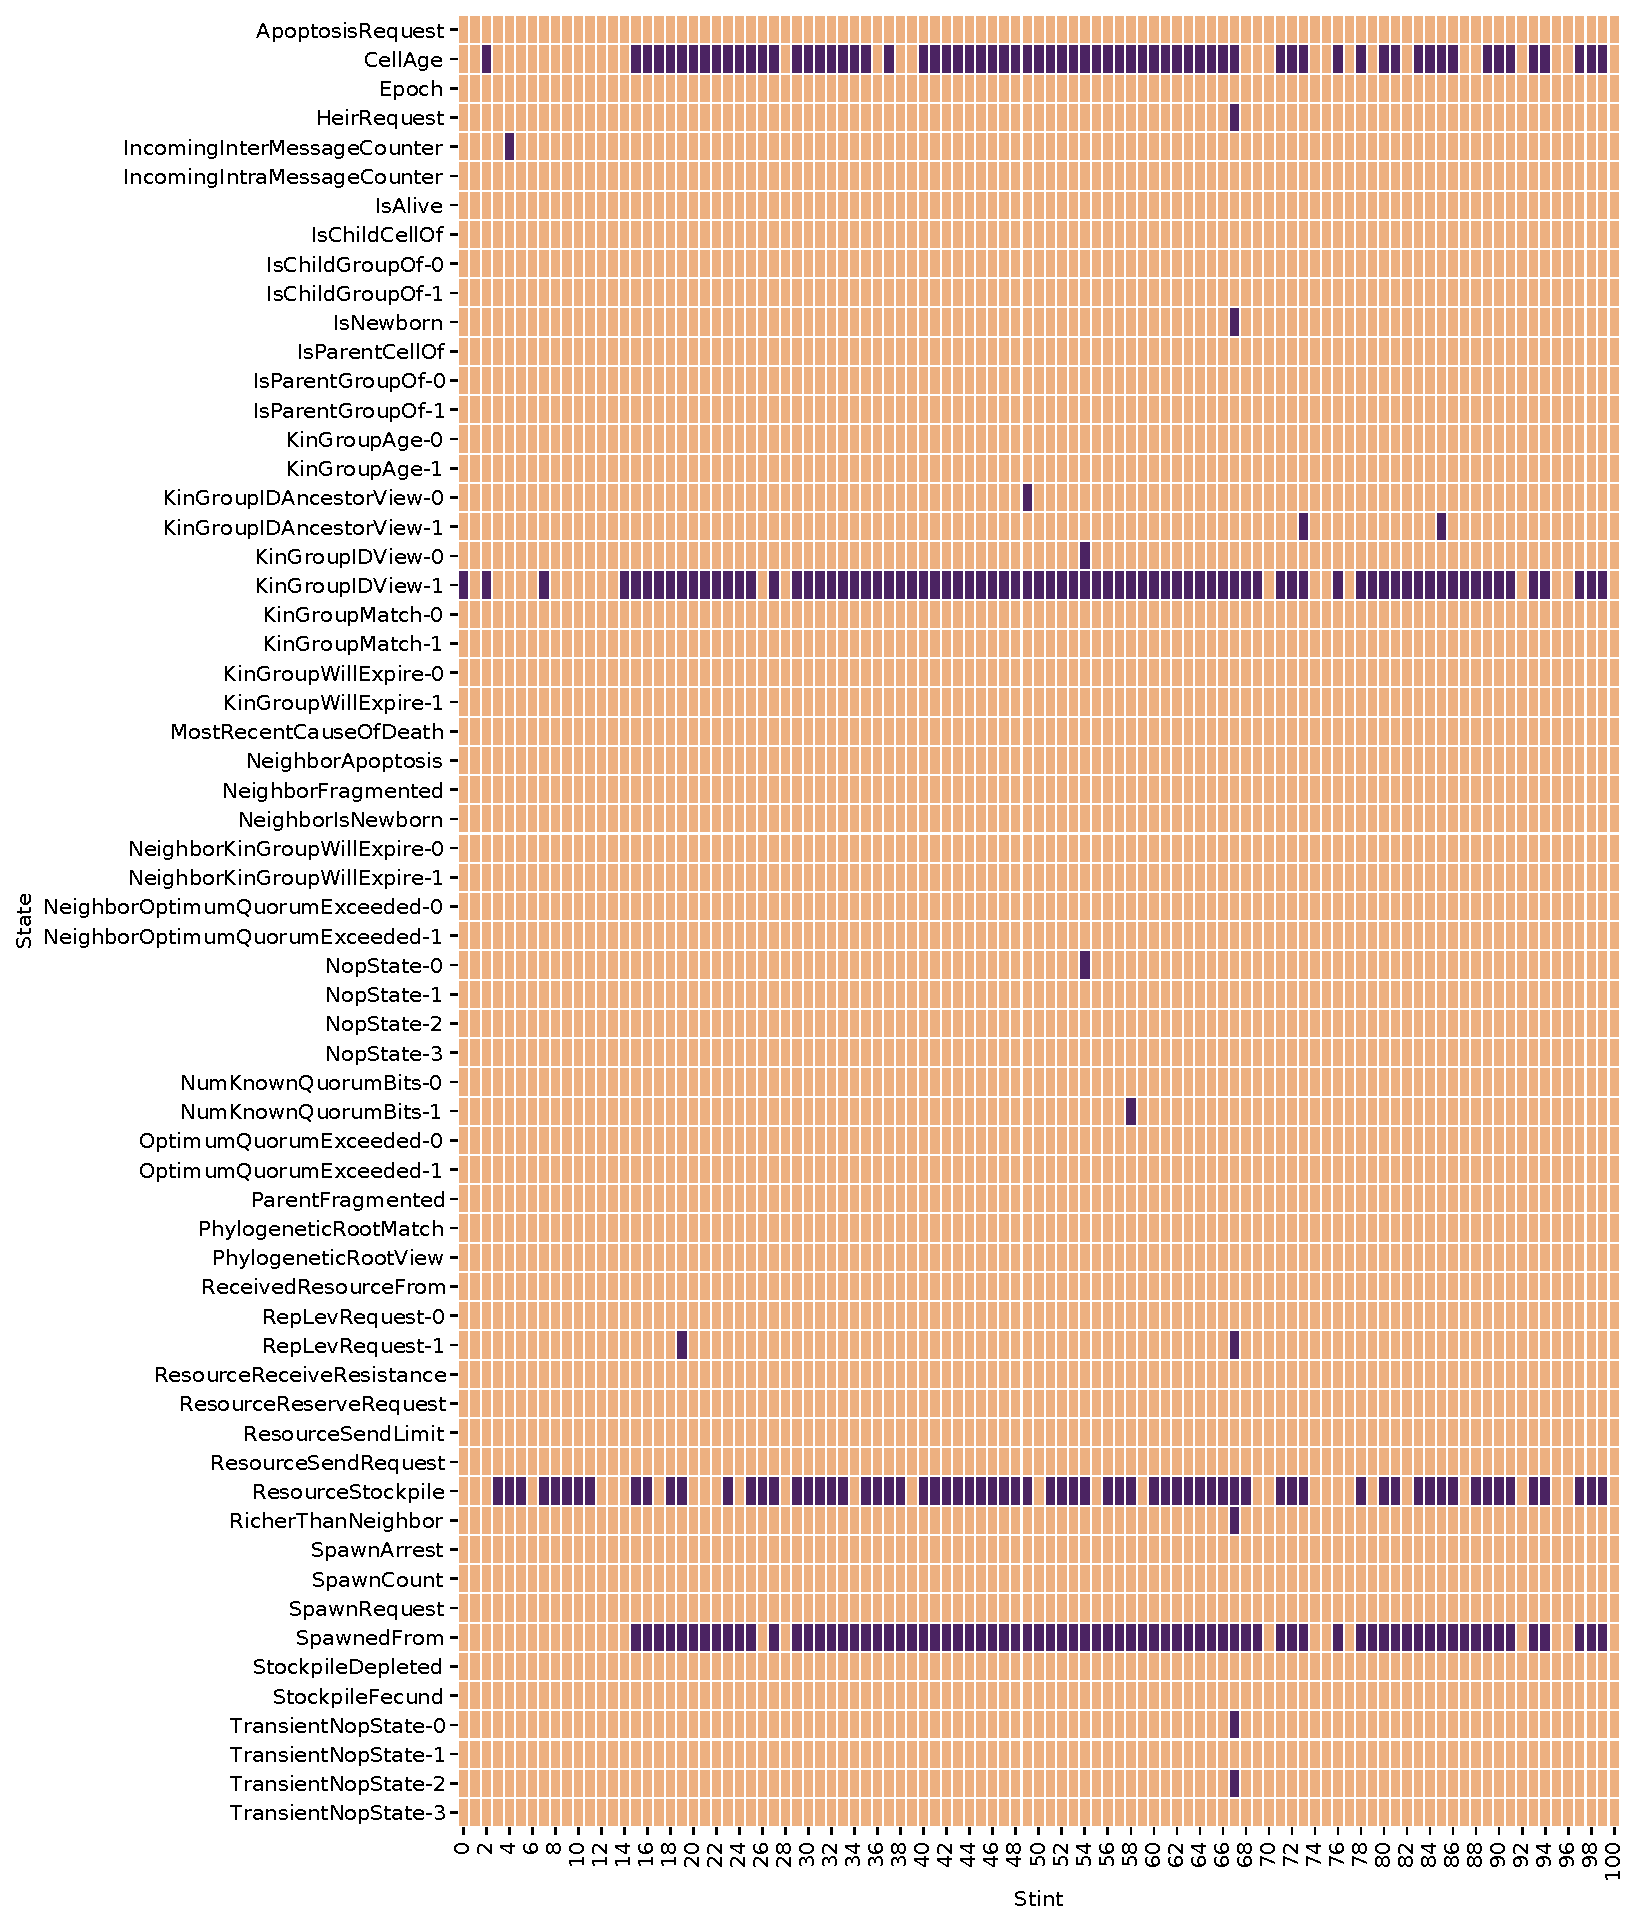
\includegraphics[width=\linewidth]{{plots/extrospective_perturbation/bucket=prq49+endeavor=16+transform=filter-Series-16005+val=extrospective-perturbation-fitness+viz=tall-heatmap+x=Stint+y=State+ext=}}

\caption{
Fitness effect of extrospective states (read-only state information of neighboring cells) for focal strains between stint 0 and 100.
Peach color indicates no fitness effect.
Burgundy indicates a significant fitness effect.
Supplementary material provides a description for each state.
}
\label{fig:extrospective_perturbation}
\end{figure*}

\begin{figure*}

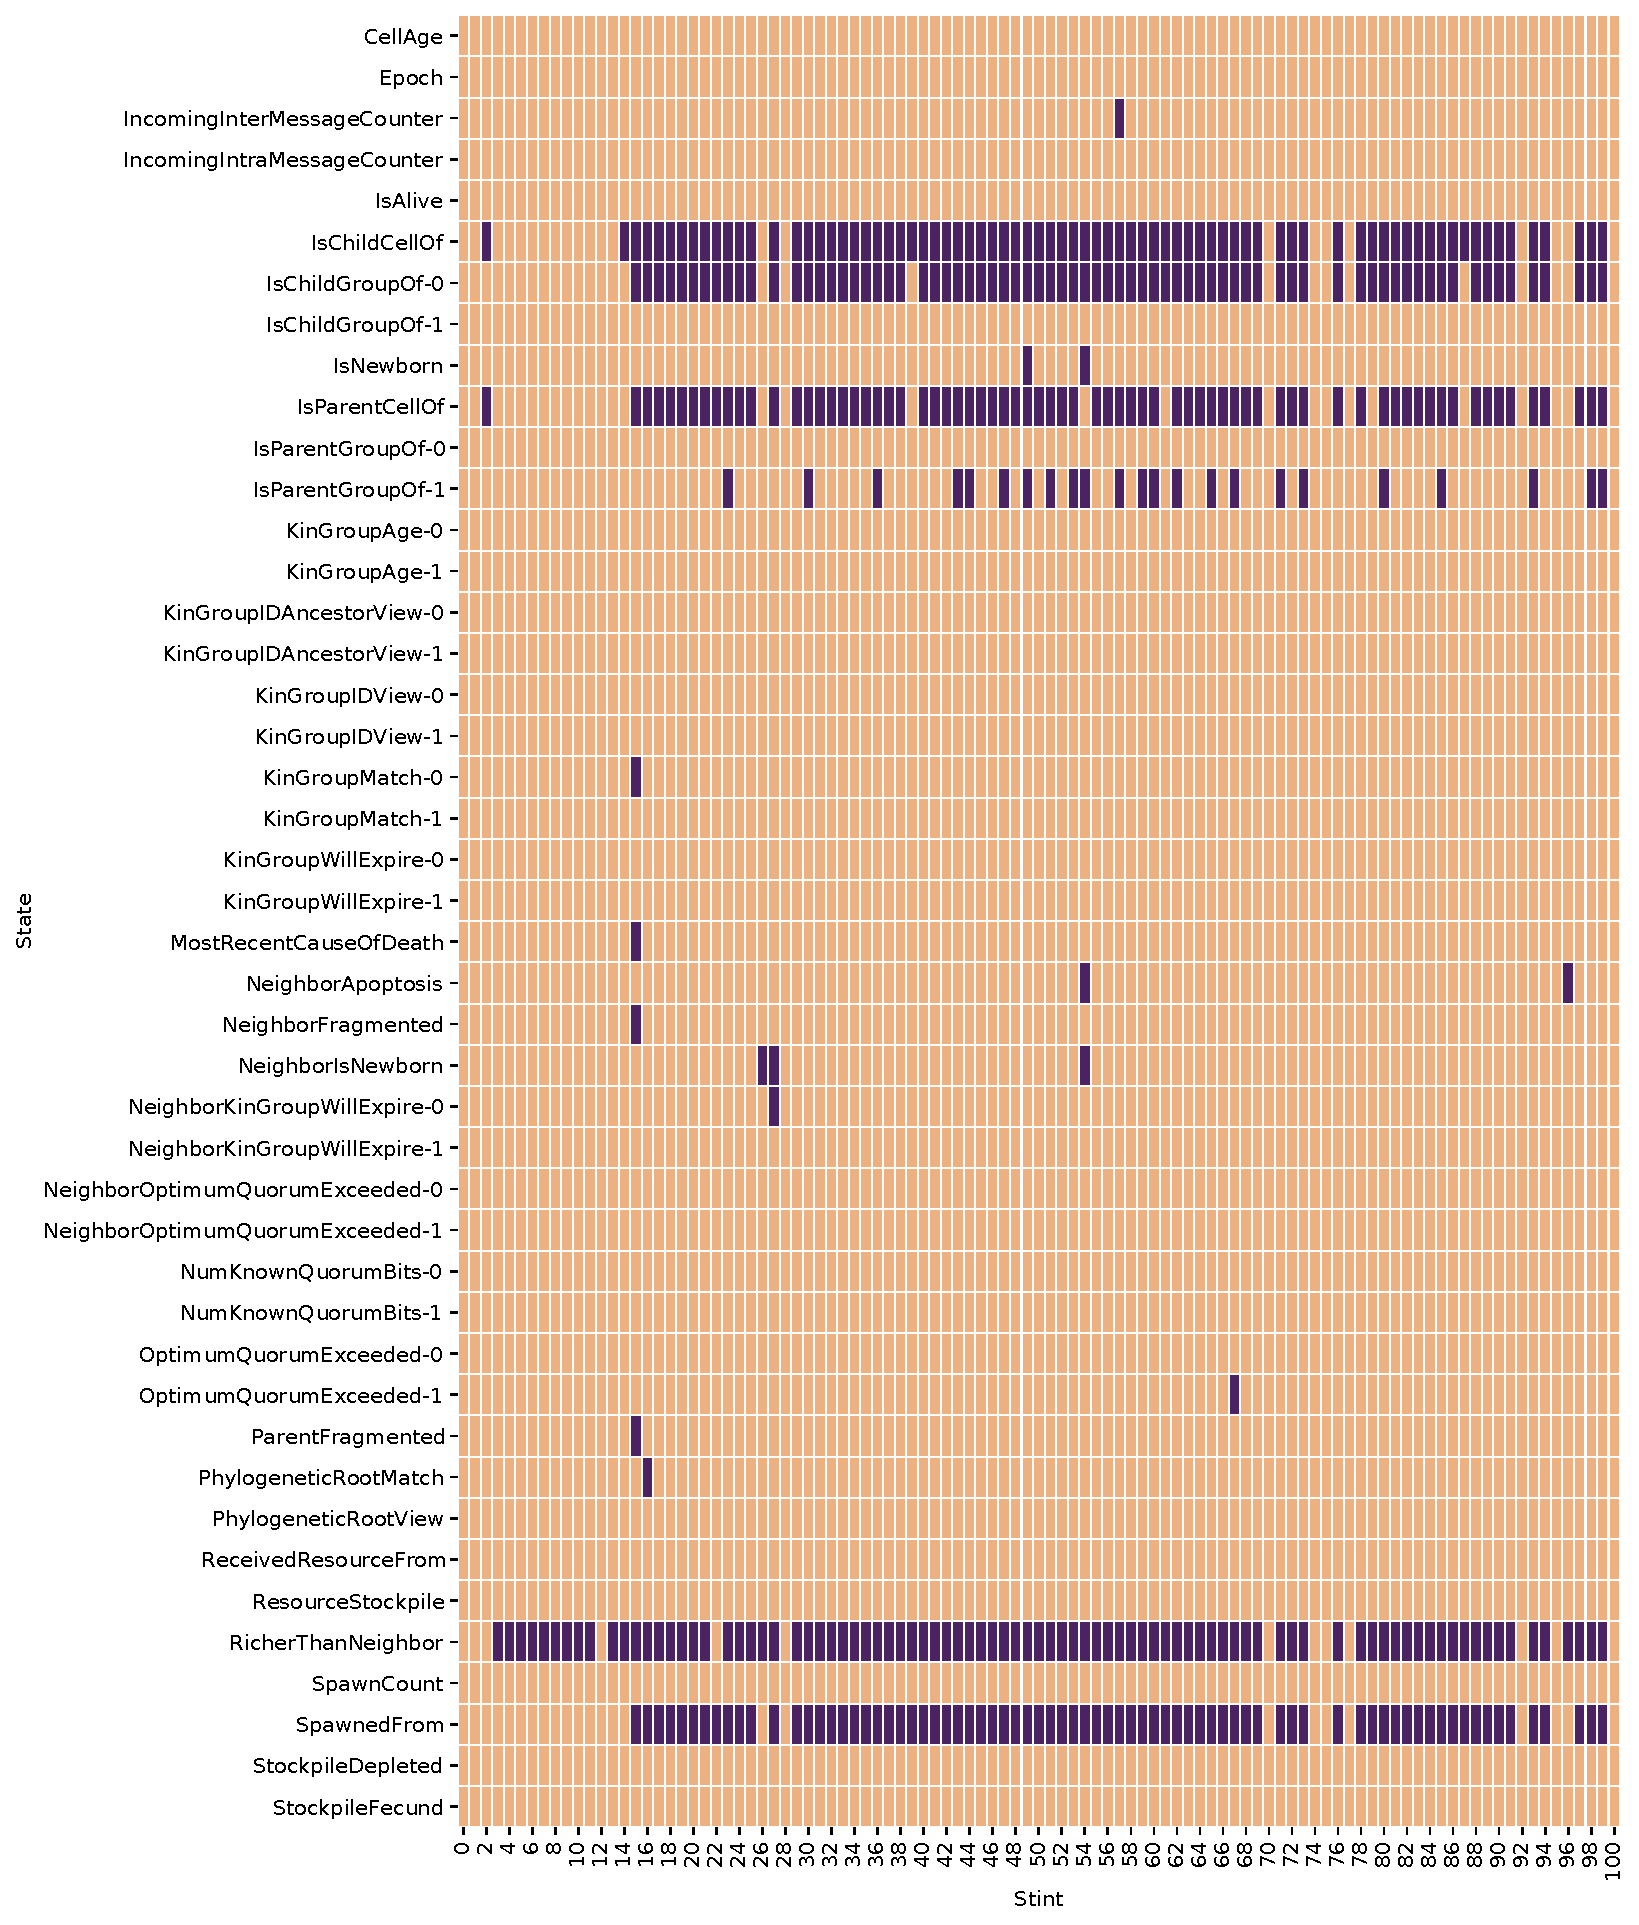
\includegraphics[width=\linewidth]{{plots/introspective_perturbation/bucket=prq49+endeavor=16+transform=filter-Series-16005+val=introspective-perturbation-fitness+viz=tall-heatmap+x=Stint+y=State+ext=}}

\caption{ Fitness effect of introspective states (state information of neighboring cells) for focal strains between stint 0 and 100.
Peach color indicates no fitness effect.
Burgundy indicates a significant fitness effect.
Supplementary material provides a description for each state. }
\label{fig:introspective_perturbation}
\end{figure*}


\begin{figure*}

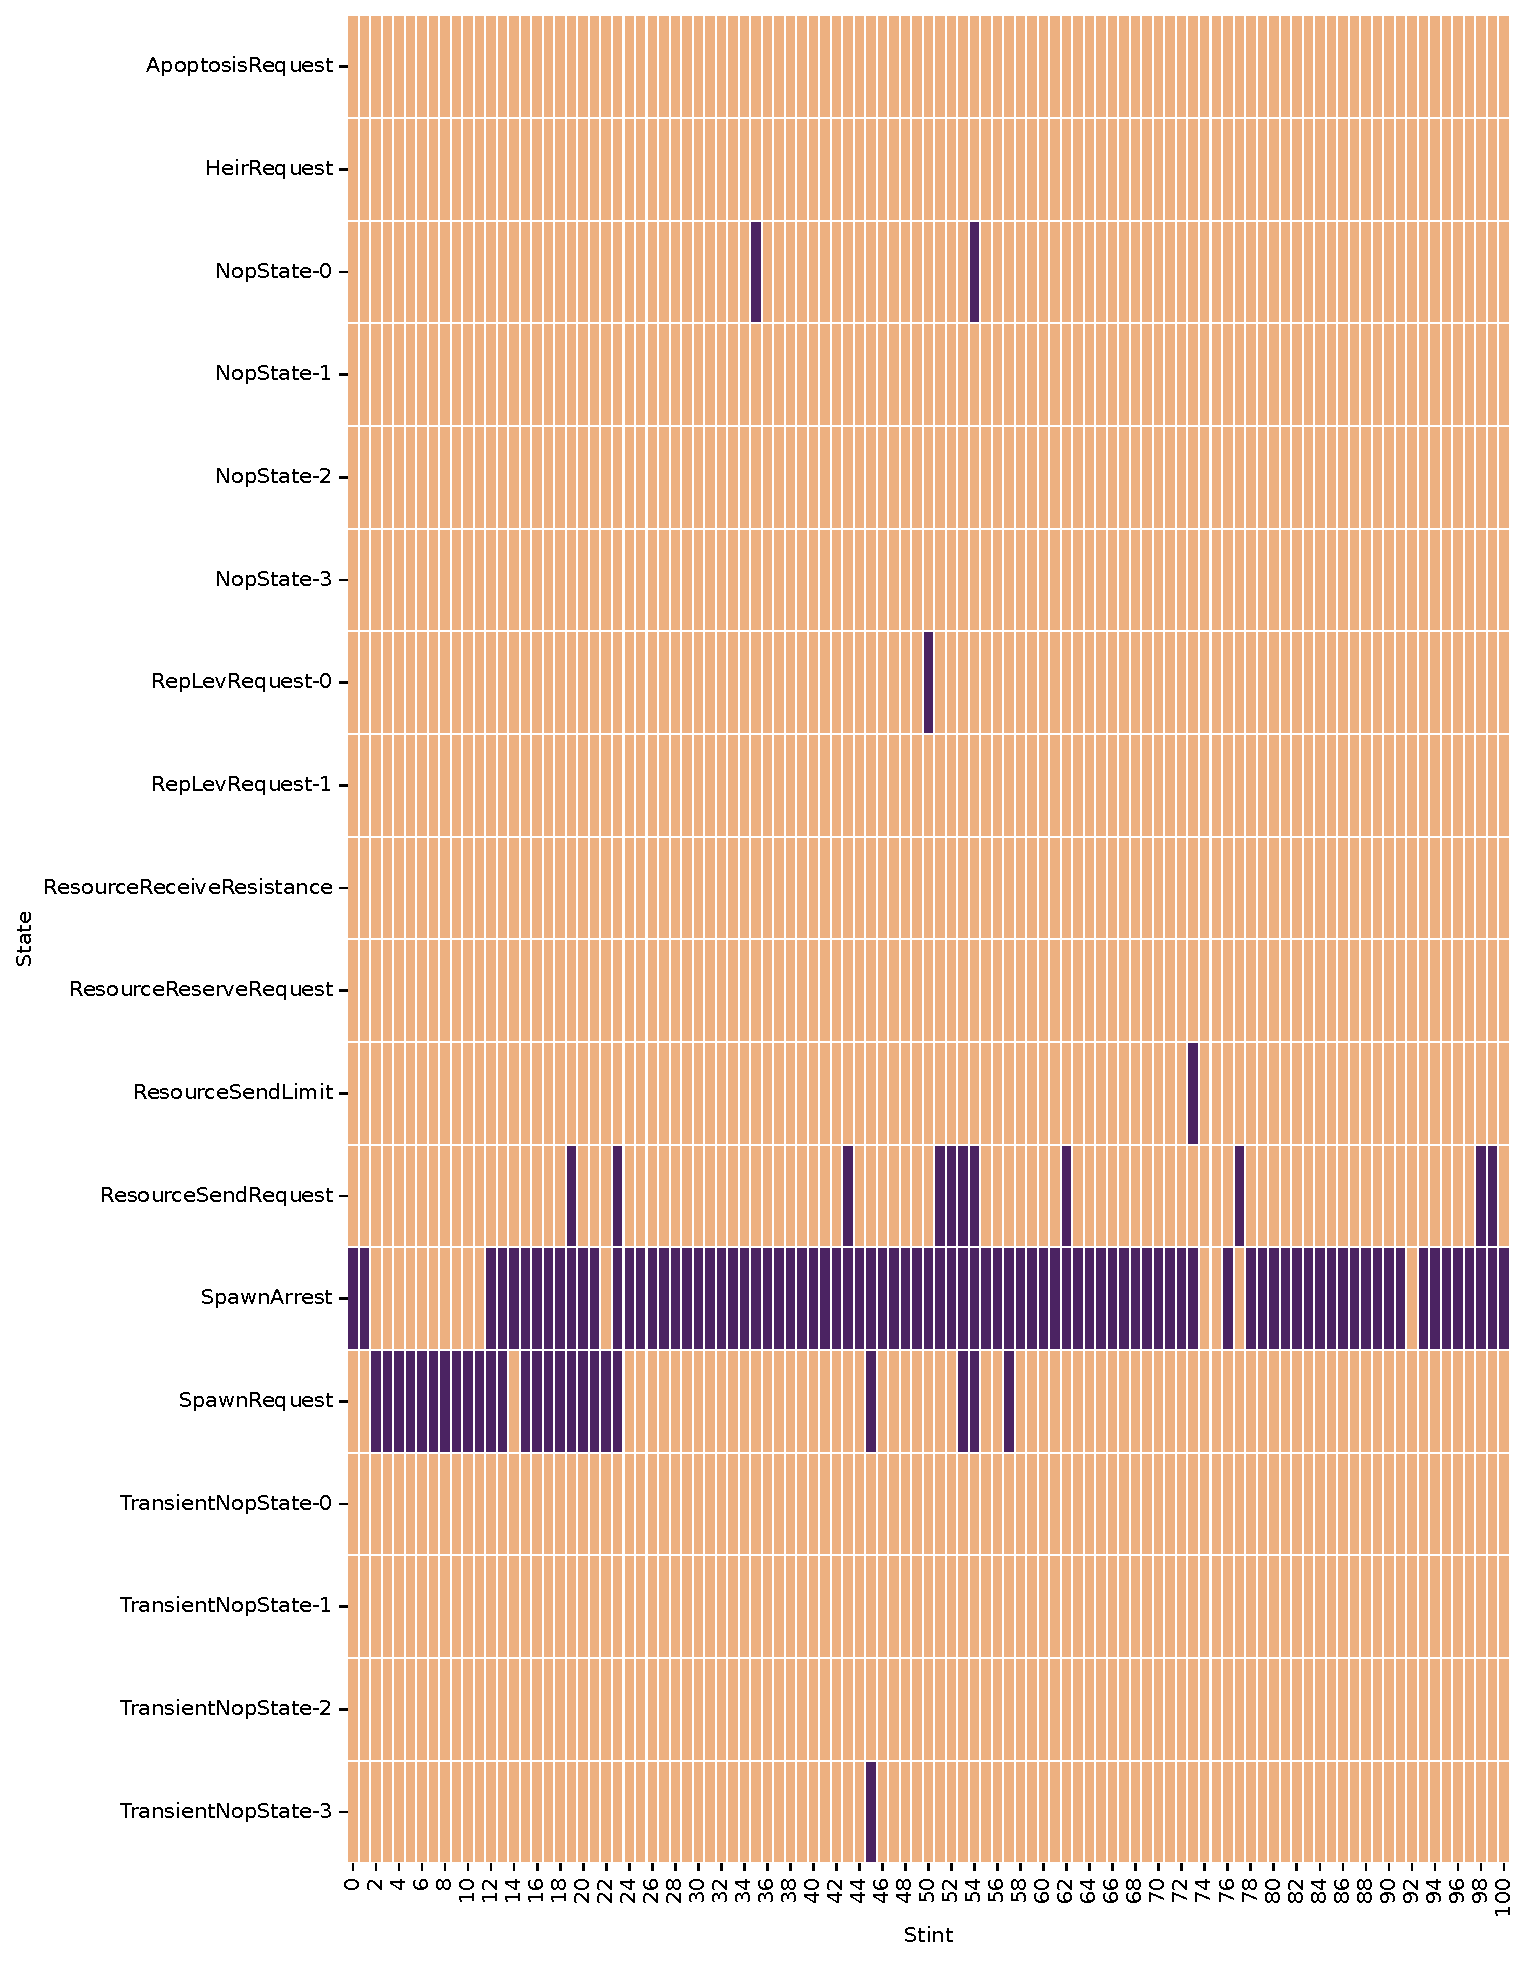
\includegraphics[width=\linewidth]{{plots/writable_perturbation/bucket=prq49+endeavor=16+transform=filter-Series-16005+val=writable-perturbation-fitness+viz=tall-heatmap+x=Stint+y=State+ext=}}

\caption{ Fitness effect of writable states (state information of neighboring cells) for focal strains between stint 0 and 100.
Peach color indicates no fitness effect.
Burgundy indicates a significant fitness effect.
Supplementary material provides a description for each state. }
\label{fig:writable_perturbation}
\end{figure*}



% \subsection{Phenotype Complexity}

% \begin{figure}

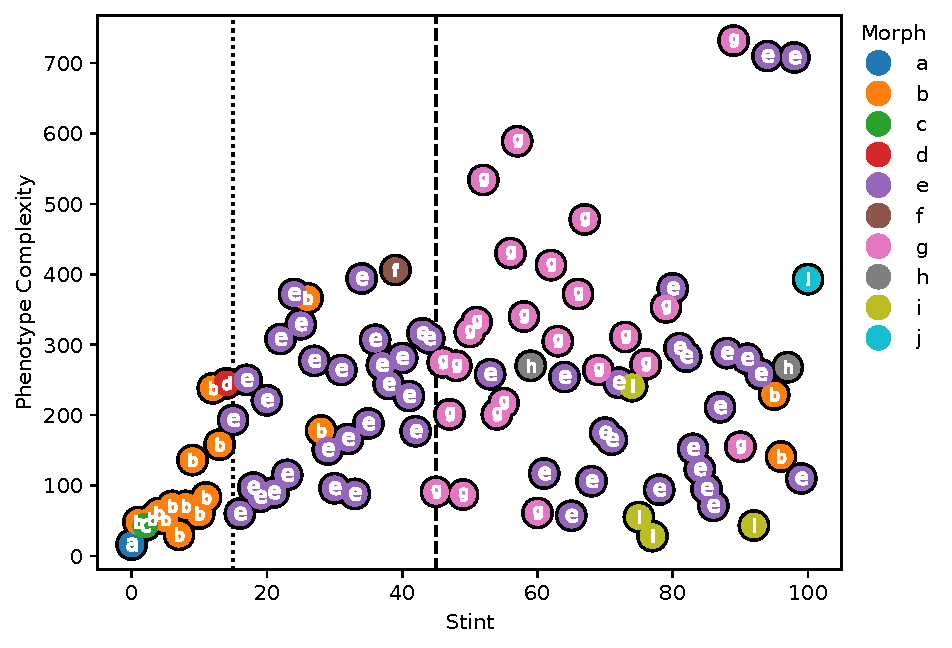
\includegraphics[width=\linewidth]{{plots/phenotype_complexity/bucket=prq49+cat=morph+endeavor=16+transform=filter-Series-16005+viz=letterscatter-vline+x=stint+y=phenotype-complexity+ext=}}

\caption{ Number of genome sites that contribute to phenotpe, measured as number sites remaining after phenotype-neutral nopout.
Color coding and letters correspond to qualitative morph codes described in Table \ref{tab:morph_descriptions}.
Dotted vertical line denotes emergence of morph $e$.
Dashed vertical line denotes emergence of morph $g$.
}
\label{fig:phenotype_complexity}
\end{figure}


% Phenotype complexity was highly volatile, bouncing at times from between more than 500 to less than 100 --- as shown in Figure \ref{fig:phenotype_complexity}.
% The maximum observed phenotype complexity was 732 sites at stint 89.

In the following sections, $L$ refers to the number of hierarchical kin group levels defined for the simulation.
In this work, we use $L=2$.

\section{Virtual CPU} \label{sec:virtual_cpu}

Each cardinal processor hosts a signalgp-lite virtual CPU \citep{lalejini2018evolving,moreno2021signalgp}.
Each CPU can host up to 16 active virtual cores.
If additional cores are required after all 16 available are in use, the oldest active core is killed and replaced.
Each virtual core contains 8 virtual \texttt{float} registers.

Cores execute round-robin in quasi-parallel, with up to 8 instructions being executed on a single core before execution shifts to the next active core.

Like SignalGP, the signalgp-lite system uses tag-matching to determine which modules to activate in response to incoming signals from the environment, from other agents (i.e., messages), and from internal events (i.e., execution of \texttt{call} and \texttt{fork} instructions).

In the DISHTINY simulation, each CPU hosts two independent module-lookup data structures.
The first module-lookup data structure is used to activate modules in response to internally-generated signals, messages from other cardinal processors within the same cell, and environmental events;
this module-lookup data structure contains \textit{all} modules within the genetic program.
The second module-lookup data structure is used to activate modules in response to messages from other cells;
this module-lookup data structure contains only modules with bitstring tags that end in 0.
(Hence, the subset of modules with bitstring tags that end in 1 \textit{cannot} be activated by messages from other cells, so that sensitive functionality like resource sharing and apoptosis can be protected from potentially malicious exploitation.)

We also use a tag-matching system to route \texttt{jump} instructions executed within a module.
When a module is loaded, all \texttt{local anchor} instructions are registered within a tag-matching data structure.
The local \texttt{jump} instruction routes to the best-matching local anchor.
If no matching local anchor is available, then no jump is performed and execution continues as if a \texttt{nop} instruction had elapsed.

\section{Tag Matching}

We use 64-bit bitstring tags to label modules and jump destinations.
We use a variant of Downing's streak metric to compute tag matches \citep{downing2015intelligence,moreno2023matchmaker}.
We deterministically select the single best-matching result for a tag lookup.
If there is a tie, an arbitrary result is selected.
For module-lookup, the best-matching tag must have a match quality at the 80th or better percentile among match qualities of pairs of randomly generated tags.
Otherwise, no module is activated.
For jump-lookup, the best match must be at the 50th or better percentile.
Otherwise, no jump is performed.

\section{Program Generation and Mutation}

Initial populations were seeded with programs consisting of 128 randomly generated instructions.
Program length was capped at 4096 instructions.

Mutation was applied to one in 10 reproductions where any kin group commonality was maintained and to 10 in 10 reproductions where it was not.
If mutation occurred, bits in the binary representation of the genome were flipped with 0.02\% probability.
If mutation occurred, sequence mutations were also introduced into the program at a per-site rate of 0.1\%.
Half of sequence mutations were deletion events, with a number of sites deleted drawn uniformly between 0 and 8.
Half of sequence mutations were insertion events, with a number of sites inserted drawn uniformly between 0 and 8.
When sites were inserted, half of the time randomly-generated instructions were added and half of the time the preceding sequence of instructions was duplicated.
With 0.1\% probability a sequence mutation took on severe intensity, meaning that the number of sites inserted or deleted was drawn uniformly between 0 and program size rather than between 0 and 8.

\section{Cooperative Resource Collection}

In order to ensure kin group structure had functional ramifications, we based part of cell resource collection on the number of contiguous kin group members.
To do this, we needed an efficient distributed method to approximate kin group size.

Each cell held a 64-bit bitstring with one chosen bit fixed.
We estimated group size by counting the number of distinct set bits (out of 64 available slots) that were contained within a kin group.
We refer to this count of distinct set bits as a group's ``quorum count.''

At every update within each tile, the simulation system broadcasts all bits that were known to be set within that tile's kin group.
This broadcast was only sent to neighboring tiles that were part of the same kin group as the broadcasting tile.
Each tile tracked which neighbor it learned of each set bit from so that when tiles left the kin group their set bits could be forgotten from the bits known to be set within the kin group.

This scheme was replicated independently for each kin group level simulated.
For the lowest-level kin group, a different fixed bit was chosen independently for each tile.
Thus, the quorum count for these lowest-level kin groups was a function of the number of cells contained.
For the highest-level kin group, each tile's fixed bit was chosen as a deterministic function of its lowest-level kin group ID.
Thus, the quorum count for these highest-level kin groups was a function of the number of lowest-level kin groups contained.

To incentivize kin group formation and maintenance, we gave each cell a 0.02 resource bonus every four updates for each non-self quorum count.
This bonus saturated at the simulation-defined target quorum count.
For both the lowest- and highest-level kin groups we used a target quorum count of 12.
The source code controlling cooperative resource collection can be found at \url{https://github.com/mmore500/dishtiny/blob/prq49/include/dish2/services/CollectiveHarvestingService.hpp}.

In addition to this cooperative resource collection mechanism, cells enjoyed a continuous resource inflow of 0.02 units per update.
The source code controlling base resource inflow can be found at \url{https://github.com/mmore500/dishtiny/blob/master/include/dish2/services/ResourceHarvestingService.hpp}.

To penalize groups that expanded beyond the simulation-defined target quorum count, we decayed held resource by a multiplicative factor of $0.9995^{2^n}$, where $n$ is the excess quorum count beyond the simulation-defined target.
The source code controlling cooperative resource collection can be found at \url{https://github.com/mmore500/dishtiny/blob/prq49/include/dish2/services/CollectiveResourceDecayService.hpp}.

In addition to any decay due to group size, held resource decayed at a rate of 0.05\% per update.
Received resource was decayed 0.099975\% upon receipt.



\section{Events}

This section enumerates simulation-managed events that were dispatched on virtual CPUs.
In addition to a program, each genome contained an array of 64-bit tags --- one for each event.
When an event's criteria was met in the simulation, the genome's corresponding tag was used to dispatch a module in the program and launch a core executing that module.

All events are also exposed to the cell as a corresponding input sensor.
The state of the event (0 for false, 1 for true) is stored in the sensor prior to virtual CPU execution.
In fact, events are triggered based on the reading of the sensor register (not by re-reading the underlying simulation state).
This means that experimental perturbations that perturb sensor input also disrupted event-handling, allowing the state interface complexity metric to measure both event-driven and sensor-based behaviors.

The source code controlling events can be found at \url{https://github.com/mmore500/dishtiny/tree/prq49/include/dish2/events} and \url{https://github.com/mmore500/dishtiny/blob/prq49/include/dish2/services/InterpretedIntrospectiveStateRefreshService.hpp}.

\subsection{Always}

This event is always dispatched.

\subsection{Is Child Cell Of}

Is this cell a daughter cell of the cardinal's neighbor?
Triggered if this cell was spawned from the cardinal's neighbor and its cell is younger than the neighbor.

\subsection{Is Child Group Of (0 thru $L-1$)}

Is this cell's kin group a daughter group of the cardinal's neighbor cell's kin group?
Triggered if a cell's kin group ancestor ID(s) are equal to the cardinal's neighbor's current kin group ID(s).

\subsection{Is Newborn}

This event is dispatched once when a cell is first born.
Triggered if cell age is less than frequency at which events are launched.

\subsection{Is Parent Cell Of}

Is this cardinal's cell the parent cell of the cardinal's neighbor?
Triggered if neighbor was spawned from cell and cell age is greater than neighbor age.

\subsection{Kin Group Match (0 thru $L-1$)}

Is this cell part of the same kin group as the cardinal's neighbor?
Triggered if a cell's kin group ID(s) are equal to the cardinal's neighbors' current kin group ID(s).

\subsection{Kin Group Mismatch (0 thru $L-1$)}

Is this cell part of a different kin group from the cardinal's neighbor cell?
Triggered if a cell's kin group ID(s) are not equal to the cardinal's neighbors' current kin group ID(s).

\subsection{Kin Group will Expire (0 thru $L-1$)}

Triggered if kin group age is greater than 80\% of the kin group expiration duration.
(Depending on experiment configuration, the group may be force-fragmented after expiration.)

\subsection{Kin Group will not Expire (0 thru $L-1$)}

Triggered if kin group age is less than or equal to than 80\% of the kin group expiration duration.

\subsection{Neighbor Apoptosis}

Triggered if the most recent cell death in the cardinal's neighbor tile was apoptosis.

\subsection{Neighbor Fragmented}

Triggered if the most recent cell death in the cardinal's neighbor tile was fragmentation.

\subsection{Neighbor Is Alive}

Triggered if a cardinal's neighbor tile is occupied by a live cell.

\subsection{Neighbor Is Newborn}

Triggered once for each time a newborn spawns into the cardinal's neighboring tile.
Triggered if the cardinal's neighbor's age is less than the frequency at which events are launched.

\subsection{Neighbor Is Not Alive}

Triggered if the cardinal's neighboring tile is not occupied.

\subsection{Neighbor Kin Group Will Expire (0 thru $L-1$)}

Triggered if the cardinal's cell neighbor's kin group age is less than or equal to 80\% of the kin group expiration duration.

\subsection{Neighbor Optimum Quorum Exceeded}

Triggered if the cardinal's cell neighbor's number of known quorum bits exceed the target quorum count.

\subsection{Optimum Quorum Exceeded (0 thru $L-1$)}

Triggered if the cell's number of known quorum bits exceed the target quorum count.

\subsection{Optimum Quorum Not Exceeded (0 thru $L-1$)}

Triggered if the cell's number of known quorum bits is less than or equal to than the target quorum count.

\subsection{Parent Fragmented}

Triggered if a cell's parent died from fragmentation.
That is, if the last cause of death on the current tile was fragmentation.

\subsection{Phylogenetic Root Match}

Does this cell descend from the same originally-generated genome as its neighbor?
Triggered if a cardinal's cell's root ID is equal to that cardinal's neighbor cell's root ID.

\subsection{Phylogenetic Root Mismatch}

Does this cell and its neighbor descend from a different originally-generated genomes?
Triggered if a cardinal's cell's root ID is not equal to that cardinal's neighbor cell's Root ID.

\subsection{Poorer Than Neighbor}

Does this cell have less resource stockpiled than its neighbor?
Triggered if a cardinal's cell has less resource than that cardinal's neighbor cell.

\subsection{Received Resource From}

Triggered if a cardinal's cell has received resource from that cardinal's neighbor cell.

\subsection{Richer Than Neighbor}

Does this cell have more resource stockpiled than its neighbor?
Triggered if a cardinal's cell has more resource in its stockpile than that cardinal's neighbor cell.

\subsection{Stockpile Depleted}

Is this cell's stockpile empty?
Triggered if a cell's stockpile is less than twice the base harvest rate.

\subsection{Stockpile Fecund}

Does this cell have enough stockpiled resource to fund cellular reproduction?
Triggered if a cell's stockpile is greater than 1.0.


\section{Operations}

% create command to draw operation tables
\newcommand{\opdef}[2]{
    \begin{tabular}{|
        >{\columncolor[HTML]{C0C0C0}}l |l|}
        \hline
        Prevalence & #1 \\ \hline
        Num Args   & #2 \\ \hline
    \end{tabular}
}

This section overviews the operation library made available to evolving signalgp-lite genetic programs within the simulation.

Within the program section of each genome, each instruction contained 
\begin{itemize}
\item an op code, specifying which operation should be performed;
\item a 64-bit bitstring, used as a tag for operations that required tag-matching or as data for some configurable operations; and
\item three integer arguments, specifying which registers the operation should apply to (many operations do not use all arguments).
\end{itemize}

In the operation descriptions below, we refer to register access via to the $n$th argument as \texttt{reg[arg\_n]}.
Each core has its own eight \texttt{float} registers.
All core registers are zeroed out at core launch.

In order to prevent bread-and-butter operations like global anchors, local anchors, and terminals from being swamped out by large instruction set size, we manually defined increased ``prevalences'' for some instructions.
This prevalence increased the probability of the operation being selected under mutations and initial program generation.
Prevalence works like increasing the number of identical copies of the operation included in the operation library.
We provide the prevalence of each operation below.

See \url{https://github.com/mmore500/dishtiny/tree/prq49/include/dish2/operations} for the source code of DISHTINY-specific operations and \url{https://github.com/mmore500/signalgp-lite/tree/b6c437f44136651aa6f4051d84bc62a86c2afbbe/include/sgpl/operations} for the source code of generic operations.

Refer to Section \ref{sec:virtual_cpu} for details on the virtual CPU running these instructions.

\subsection{Fork If}

\opdef{1}{1}

If \texttt{reg[arg\_0]} is nonzero, registers a request to activate a new core with the module best-matching the current instruction's tag.
These fork requests are only handled when the current core terminates.
Each core may only register 3 fork requests.

\subsection{Nop, 0 RNG Touches}

\opdef{1}{0}

Performs no operation for one virtual CPU cycle.

\subsection{Nop, 1 RNG Touches}

\opdef{1}{0}

Performs no operation for one virtual CPU cycle, and advances the RNG engine once.
(Important to nop-out operations that perform one RNG touch without causing side effects.)

\subsection{Nop, 2 RNG Touches}

\opdef{1}{1}

Performs no operation for one virtual CPU cycle, and advances the RNG engine twice.
(Important to nop-out operations that perform two RNG touches without causing side effects.)

\subsection{Terminate If}

\opdef{1}{1}

Terminates current core if \texttt{reg[arg\_0]} is nonzero.

\subsection{Add}

\opdef{1}{3}

Adds \texttt{reg[arg\_1]} to \texttt{reg[arg\_2]} and stores the result in \texttt{reg[arg\_0]}.

\subsection{Divide}

\opdef{1}{3}

Divides \texttt{reg[arg\_1]} by \texttt{reg[arg\_2]} and stores the result in \texttt{reg[arg\_0]}.
Division by zero can result in an \texttt{Inf} or \texttt{NaN} value.

\subsection{Modulo}

\opdef{1}{3}

Calculates the modulus of \texttt{reg[arg\_1]} by \texttt{reg[arg\_2]} and stores the result in \texttt{reg[arg\_0]}.
Mod by zero can result in a \texttt{NaN} value.

\subsection{Multiply}

\opdef{1}{3}

Multiplies \texttt{reg[arg\_1]} by \texttt{reg[arg\_2]} and stores the result in \texttt{reg[arg\_0]}.

\subsection{Subtract}

\opdef{1}{3}

Subtracts \texttt{reg[arg\_2]} from \texttt{reg[arg\_1]} and stores the result in \texttt{reg[arg\_0]}.

\subsection{Bitwise And}

\opdef{1}{3}

Performs a bitwise AND of \texttt{reg[arg\_1]} and \texttt{reg[arg\_2]} then stores the result in \texttt{reg[arg\_0]}.

\subsection{Bitwise Not}

\opdef{1}{2}

Computes the bitwise NOT of \texttt{reg[arg\_1]} and stores the result in \texttt{reg[arg\_0]}.

\subsection{Bitwise Or}

\opdef{1}{3}

Performs a bitwise OR of \texttt{reg[arg\_1]} and \texttt{reg[arg\_2]} then stores the result in \texttt{reg[arg\_0]}.

\subsection{Bitwise Shift}

\opdef{1}{3}

Shifts the bits of \texttt{reg[arg\_1]} by \texttt{reg[arg\_2]} positions.
(If \texttt{reg[arg\_2]} is negative, this is a right shift.
Otherwise it is a left shift.)
Stores the result in \texttt{reg[arg\_0]}.

\subsection{Bitwise Xor}

\opdef{1}{3}

Performs a bitwise XOR of \texttt{reg[arg\_1]} and \texttt{reg[arg\_2]} then stores the result in \texttt{reg[arg\_0]}.

\subsection{Count Ones}

\opdef{1}{2}

Counts the number of bits set in \texttt{reg[arg\_1]} and stores the result in \texttt{reg[arg\_0]}.

\subsection{Random Fill}

\opdef{1}{1}

Fills register pointed to by \texttt{reg[arg\_0]} with random bits chosen from a uniform distribution.

\subsection{Equal}

\opdef{1}{3}

Checks whether \texttt{reg[arg\_1]} is equal to \texttt{reg[arg\_2]} and stores the result in \texttt{reg[arg\_0]}.

\subsection{Greater Than}

\opdef{1}{3}

Checks whether \texttt{reg[arg\_1]} is greater than \texttt{reg[arg\_2]} and stores the result in \texttt{reg[arg\_0]}.

\subsection{Less Than}

\opdef{1}{3}

Checks whether \texttt{reg[arg\_1]} is less than \texttt{reg[arg\_2]} and stores the result in \texttt{reg[arg\_0]}.

\subsection{Logical And}

\opdef{1}{3}

Performs a logical AND of \texttt{reg[arg\_1]} and \texttt{reg[arg\_2]}, storing the result in \texttt{reg[arg\_0]}.

\subsection{Logical Or}

\opdef{1}{3}

Performs a logical OR of \texttt{reg[arg\_1]} and \texttt{reg[arg\_2]}, storing the result in \texttt{reg[arg\_0]}.

\subsection{Not Equal}

\opdef{1}{3}

Checks whether \texttt{reg[arg\_1]} is not equal to \texttt{reg[arg\_2]} and stores the result in \texttt{reg[arg\_0]}.

\subsection{Global Anchor} \label{sec:global_anchor}

\opdef{15}{0}

Marks a module-begin position.
Based on tag-lookup, new cores or global jump instructions may set the program counter to this instruction's program position.

This instruction can also mark a module-end position --- executing this instruction can terminate the executing core.
If no local anchor instruction is present between the current global anchor instruction and the preceding global anchor instruction, this operation will not terminate the executing core.
(This way, several global anchors may lead into the same module.)

However, if a local anchor instruction is present between the current global anchor instruction and the preceding global anchor instruction, this operation will terminate the executing core. 
Local jump instructions will only consider local anchors between the preceding global anchor and the subsequent global anchor instruction.

\subsection{Global Jump If}

\opdef{1}{2}

Jumps the current core to a global anchor that matches the instruction tag if \texttt{reg[arg\_0]} is nonzero.
If \texttt{reg[arg\_1]} is nonzero, resets registers.

\subsection{Global Jump If Not}

\opdef{1}{2}

Jumps the current core to a global anchor that matches the instruction tag if \texttt{reg[arg\_0]} is nonzero.
If \texttt{reg[arg\_1]} is zero, resets registers.

\subsection{Protected Regulator Adjust}

\opdef{1}{1}

Adjusts the regulator value of global jump table tags matching this instruction's tag by the amount \texttt{reg[arg\_0]}.

This regulator value affects the outcome of tag lookup for internal events and signals from the environment.
(Note, as described in \ref{sec:virtual_cpu}, that independent tag lookup tables handle activating genome modules across different contexts.)

\subsection{Protected Regulator Decay}

\opdef{1}{1}

Ages the regulator decay countdown of global jump table tags matching this instruction's tag by the amount \texttt{reg[arg\_0]}.
If \texttt{reg[arg\_0]} is negative, this can forestall decay. 

This decay countdown affects the outcome of tag lookup for internal events, and signals from the environment.
(Note, as described in \ref{sec:virtual_cpu}, that independent tag lookup tables handle activating genome modules across different contexts.)

\subsection{Protected Regulator Get}

\opdef{1}{1}

Gets the regulator value of the global jump table tag that best matches this instruction's tag.
Stores the value in \texttt{reg[arg\_0]}.

If no tag matches, a no-op is performed.

The regulator value gotten controls internal events and signals from the environment.
(Note, as described in \ref{sec:virtual_cpu}, that independent tag lookup tables handle activating genome modules across different contexts.)

\subsection{Protected Regulator Set}

\opdef{1}{1}

Sets the regulator value of global jump table tags matching this instruction's tag to \texttt{reg[arg\_0]}.

This regulator value affects the outcome of tag lookup for internal events and signals from the environment.
(Note, as described in \ref{sec:virtual_cpu}, that independent tag lookup tables handle activating genome modules across different contexts.)

\subsection{Local Anchor}

\opdef{20}{0}

Marks a program location local jump instructions may route to.
This program location is tagged with the instruction's tag.

As described in Section \ref{sec:global_anchor}, this operation also plays a role in determining whether global anchor instructions close a module.

\subsection{Local Jump If}

\opdef{1}{1}

Jumps to a local anchor that matches the instruction tag if \texttt{reg[arg\_0]} is nonzero.

\subsection{Local Jump If Not}

\opdef{1}{1}

Jumps to a local anchor that matches the instruction tag if \texttt{reg[arg\_0]} is zero.

\subsection{Local Regulator Adjust}

\opdef{1}{1}

Adjusts the regulator value of local jump table tags matching this instruction's tag by the amount \texttt{reg[arg\_0]}.

\subsection{Local Regulator Decay}

\opdef{1}{1}

Ages the regulator decay countdown of local jump table tags matching this instruction's tag by the amount \texttt{reg[arg\_0]}.
If \texttt{reg[arg\_0]} is negative, this can forestall decay.

\subsection{Local Regulator Get}

\opdef{1}{1}

Gets the regulator value of the local jump table tag that best matches this instruction's tag.
Stores the value in \texttt{reg[arg\_0]}.

If no tag matches, a no-op is performed.

\subsection{Local Regulator Set}

\opdef{1}{1}

Sets the regulator value of global jump table tags matching this instruction's tag to \texttt{reg[arg\_0]}.

\subsection{Decrement}

\opdef{1}{1}

Takes \texttt{reg[arg\_0]}, decrements it by one, and stores the result in \texttt{reg[arg\_0]}.

\subsection{Increment}

\opdef{1}{1}

Takes \texttt{reg[arg\_0]}, increments it by one, and stores the result in \texttt{reg[arg\_0]}.

\subsection{Negate}

\opdef{1}{1}

Negates \texttt{reg[arg\_0]} and stores the result in \texttt{reg[arg\_0]}.

\subsection{Not}

\opdef{1}{1}

Performs a logical not on \texttt{reg[arg\_0]} and stores the result in \texttt{reg[arg\_0]}.

\subsection{Random Bool}

\opdef{1}{1}

Stores \texttt{1.0f} to \texttt{reg[arg\_0]} with probability determined by this instruction's tag.
Otherwise, stores \texttt{0.0f} to \texttt{reg[arg\_0]}.

\subsection{Random Draw}

\opdef{1}{1}

Stores a randomly drawn float value to \texttt{reg[arg\_0]}.

\subsection{Terminal}

\opdef{50}{1}

Stores a genetically-encoded value to \texttt{reg[arg\_0]}.
This value is determined deterministically using the instruction's tag.

\subsection{Exposed Regulator Adjust}

\opdef{1}{1}

Adjusts the regulator value of global jump table tags matching this instruction's tag by the amount \texttt{reg[arg\_0]}.

This regulator value affects the outcome of tag lookup for messages from neighbor cells.
(Note, as described in \ref{sec:virtual_cpu}, that independent tag lookup tables handle activating genome modules across different contexts.)

\subsection{Exposed Regulator Decay}

\opdef{1}{1}

Ages the regulator decay countdown of global jump table tags matching this instruction's tag by the amount \texttt{reg[arg\_0]}.
If \texttt{reg[arg\_0]} is negative, this can forestall decay. 

This decay countdown affects the outcome of tag lookup for messages from neighbor cells.
(Note, as described in \ref{sec:virtual_cpu}, that independent tag lookup tables handle activating genome modules across different contexts.)

\subsection{Exposed Regulator Get}

\opdef{1}{1}

Gets the regulator value of the global jump table tag that best matches this instruction's tag.
Stores the value in \texttt{arg[0]}.

If no tag matches, a no-op is performed.

The regulator value gotten controls messages from other cells.
(Note, as described in \ref{sec:virtual_cpu}, that independent tag lookup tables handle activating genome modules across different contexts.)

\subsection{Exposed Regulator Set}

\opdef{1}{1}

Sets the regulator value of global jump table tags matching this instruction's tag to \texttt{reg[arg\_0]}.

This regulator value affects the outcome of tag lookup for messages from other cells.
(Note, as described in \ref{sec:virtual_cpu}, that independent tag lookup tables handle activating genome modules across different contexts.)

\subsection{Add to Own State}

\opdef{5}{1}

Adds \texttt{reg[arg\_0]} to the current value in a target writable state then stores the sum back in to that target writable state.

To determine the target writable state, interprets the first 32 bits of the instruction tag as an unsigned integer then calculates the remainder of integer division by the number of writable states.

\subsection{Broadcast Intra Message If}

\opdef{1}{1}

If \texttt{reg[arg\_0]} is nonzero, generates a message tagged with the instruction's tag that contains the core's current register state.
Broadcasts this message to every other cardinal within the cell.

\subsection{Multiply Own State}

\opdef{5}{1}

Multiplies \texttt{reg[arg\_0]} by the current value in a target writable state then stores the result back in to that target writable state.

To determine the target writable state, interprets the first 32 bits of the instruction tag as an unsigned integer then calculates the remainder of integer division by the number of writable states.

\subsection{Read Neighbor State}

\opdef{10}{1}

Reads a target readable state from the neighboring cell and stores it into \texttt{reg[arg\_0]}.

To determine the target readable state, interprets the first 32 bits of the instruction tag as an unsigned integer then calculates the remainder of integer division by the number of readable states.

\subsection{Read Own State}

\opdef{20}{1}

Reads a target readable state and stores it into \texttt{reg[arg\_0]}.

To determine the target readable state, interprets the first 32 bits of the instruction tag as an unsigned integer then calculates the remainder of integer division by the number of readable states.

\subsection{Send Inter Message If}

\opdef{5}{1}

If \texttt{reg[arg\_0]} is nonzero, generates a message tagged with the instruction's tag that contains the core's current register state.
Sends this message to the neighboring cell.

\subsection{Send Intra Message If}

\opdef{5}{1}

If \texttt{reg[arg\_0]} is nonzero, generates a message tagged with the instruction's tag that contains the core's current register state.
Sends this message to a target cardinal within the cell.

To determine the target cardinal, sums instruction arguments then calculates the remainder of integer division by the number of co-cardinals.

\subsection{Write Own State If}

\opdef{5}{2}

If \texttt{reg[arg\_1]} is nonzero, stores \texttt{reg[arg\_0]} into a target writable state.

To determine the target writable state, interprets the first 32 bits of the instruction tag as an unsigned integer then calculates the remainder of integer division by the number of writable states.


% create command to draw state tables
\newcommand{\instrospectivestatedef}[2]{
    \begin{tabular}{|
        >{\columncolor[HTML]{C0C0C0}}l |l|}
        \hline
        Type & #1 \\ \hline
        Category & #2 \\ \hline
    \end{tabular} \\
}

\section{Introspective State}

Introspective state refers to the collection of simulation-generated sensor values that evolving programs running within each cardinal processor can access via read-only operations.
Each cardinal processor has an independent copy of each piece of introspective state state.
(However, some introspective states representing cell state are set to identical values across cardinal processors within the same cell.)

Each cardinal processor's introspective state regularly copied and dispatched to that cardinal processor's neighbor cell, where it serves as read-only extrospective state.

Introspective state is organized into two categories:
\begin{enumerate}
    \item raw introspective state, and
    \item interpreted introspective state.
\end{enumerate}

Raw introspective state directly exposes aspects of simulation state.
Interpreted introspective state is filled with truthy values that are interpreted as booleans to dispatch environmentally-managed events.

See \url{https://github.com/mmore500/dishtiny/tree/prq49/include/dish2/peripheral/readable_state/introspective_state} for source code implementing introspective state.

\subsection{Is Child Cell Of}

\instrospectivestatedef{\texttt{char} (w/ boolean semantics)}{interpreted}

Did this cell spawn from this cardinal processor's neighbor cell?

\subsection{Is Child Group Of (0 thru $L-1$)}

\instrospectivestatedef{\texttt{char} (w/ boolean semantics)}{interpreted}

Does this cell's kin group ID descend directly from the neighbor's kin group ID?

\subsection{Is Newborn}

\instrospectivestatedef{\texttt{char} (w/ boolean semantics)}{interpreted}

Is this cell's age less than \texttt{EVENT\_LAUNCHING\_SERVICE\_FREQUENCY}?

\subsection{Is Parent Cell Of}

\instrospectivestatedef{\texttt{char} (w/ boolean semantics)}{interpreted}

Did this cardinal processor's neighbor cell spawn from this cell?
That is, was neighbor was spawned from this cell and is this cell older than neighbor?

\subsection{Is Parent Group Of}

\instrospectivestatedef{\texttt{char} (w/ boolean semantics)}{interpreted}

Did this cell's kin group descend directly from the cardinal processor's neighbor cell's kin group?
That is, is cell's kin group ancestor ID(s) equal to the cardinal processor's neighbor's current kin group ID(s).

\subsection{Kin Group Match (0 thru $L-1$)}

\instrospectivestatedef{\texttt{char} (w/ boolean semantics)}{interpreted}

Does this cell's kin group ID match the neighbor's kin group ID?

\subsection{Kin Group will Expire (0 thru $L-1$)}

\instrospectivestatedef{\texttt{char} (w/ boolean semantics)}{interpreted}

Is this cell's kin group age greater than 80\% of this level's \texttt{GROUP\_EXPIRATION\_DURATIONS}?

\subsection{Neighbor Apoptosis}

Was the neighbor tile's most recent death apoptosis?

\instrospectivestatedef{\texttt{char} (w/ boolean semantics)}{interpreted}

\subsection{Neighbor Fragmented}

Was group fragmentation the most recent cause of death in the cardinal processor's neighbor cell?

\instrospectivestatedef{\texttt{char} (w/ boolean semantics)}{interpreted}

\subsection{Neighbor Is Newborn}

\instrospectivestatedef{\texttt{char} (w/ boolean semantics)}{interpreted}

Is the neighbor's cell age less than \texttt{EVENT\_LAUNCHING\_SERVICE\_FREQUENCY}?

\subsection{Neighbor Kin Group Will Expire (0 thru $L-1$)}{interpreted}

\instrospectivestatedef{\texttt{char} (w/ boolean semantics)}{interpreted}

Is this cell's kin group age greater than 80\% of the this level's \texttt{GROUP\_EXPIRATION\_DURATIONS}?

\subsection{Neighbor Optimum Quorum Exceeded (0 thru $L-1$)}

\instrospectivestatedef{\texttt{char} (w/ boolean semantics)}{interpreted}

Is this cardinal processor's neighbor cell's kin group quorum count more than the simulation-defined target count \texttt{OPTIMAL\_QUORUM\_COUNT}?

\subsection{Optimum Quorum Exceeded (0 thru $L-1$)}

\instrospectivestatedef{\texttt{char} (w/ boolean semantics)}{interpreted}

Is this cell's kin group quorum count more than the simulation-defined target count \texttt{OPTIMAL\_QUORUM\_COUNT}?

\subsection{Parent Fragmented}

\instrospectivestatedef{\texttt{char} (w/ boolean semantics)}{interpreted}

Did the cell's parent die from fragmentation?
That is, was the last cause of death on the current tile was fragmentation?

\subsection{Phylogenetic Root Match}

\instrospectivestatedef{\texttt{char} (w/ boolean semantics)}{interpreted}

Does this cell's root ID equal the cardinal processor's cell neighbor's root ID?
(This means they originate from the same seed ancestor.)

\subsection{Richer Than Neighbor}

\instrospectivestatedef{\texttt{char} (w/ boolean semantics)}{interpreted}

Does this cell's stockpile more resource than the cardinal processor's cell neighbor?

\subsection{Stockpile Depleted}

\instrospectivestatedef{\texttt{char} (w/ boolean semantics)}{interpreted}

Is this cell's stockpile less than twice the base harvest rate?

\subsection{Stockpile Fecund}

\instrospectivestatedef{\texttt{char} (w/ boolean semantics)}{interpreted}

Does this cell have enough resource stockpiled to fund spawning an offspring cell?

\subsection{Cell Age}

\instrospectivestatedef{\texttt{size\_t}}{raw}

Number CellAgeService calls elapsed since cell was born.

\subsection{Epoch}

\instrospectivestatedef{\texttt{size\_t}}{raw}

Updates elapsed since start of simulation.

\subsection{Incoming Inter Message Counter}

\instrospectivestatedef{\texttt{size\_t}}{raw}

Counter tracking incoming messages from cardinal processor's neighbor cell.
Intermittently reset to zero.

\subsection{Incoming Intra Message Counter}

\instrospectivestatedef{\texttt{size\_t}}{raw}

Counter of incoming messages from other cardinal processors within the cell.
Intermittently reset to zero.

\subsection{Is Alive}

\instrospectivestatedef{\texttt{char} (w/ boolean semantics)}{raw}

Whether the cell is alive.
Although trivial as introspective state, this state is useful for neighbor cell's extrospective state.

\subsection{Kin Group Age ($0$ thru $L - 1$)}

\instrospectivestatedef{\texttt{size\_t}}{raw}

Number of epochs elapsed since kin group formation.

\subsection{Kin Group ID Ancestor View ($0$ thru $L - 1$)}

\instrospectivestatedef{\texttt{size\_t}}{raw}

Kin group ID from which cell's kin group ID is descended.

\subsection{Kin Group ID View ($0$ thru $L - 1$)}

\instrospectivestatedef{\texttt{size\_t}}{raw}

Kin group ID of this cell.

\subsection{Most Recent Cause of Death}{raw}

\instrospectivestatedef{\texttt{char}}{raw}

What was this the most recent cause of death on this tile?
Encoded using the \texttt{CauseOfDeath} enum.

\subsection{Num Known Quorum Bits (0 thru $L-1$)}

\instrospectivestatedef{\texttt{size\_t}}{raw}

What is this cell's known quorum count?
(How many unique quorum bits collected from kin group members are known?)

\subsection{Phylogenetic Root View}

\instrospectivestatedef{\texttt{size\_t}}{raw}

What is this cell's phylogenetic root ID?

(Which initially-generated ancestor is this cell descended from?)

\subsection{Received Resource From}

\instrospectivestatedef{\texttt{float}}{raw}

How much resource is being received from the cardinal processor's cell neighbor?

\subsection{Resource Stockpile}

\instrospectivestatedef{\texttt{float}}{raw}

Amount of resource this cell has.

\subsection{Spawn Count}

\instrospectivestatedef{\texttt{float}}{raw}

Number of offspring generated from this cell and sent to the cardinal processor's neighbor tile.
Includes offspring that do not successfully take into the neighbor tile or have not survived.

\subsection{Spawned From}

\instrospectivestatedef{\texttt{char} (w/ boolean semantics)}{raw}

Did this cell spawn from this cardinal processor's neighbor cell?


% create command to draw state tables
\newcommand{\writablestatedef}[2]{
    \begin{tabular}{|
        >{\columncolor[HTML]{C0C0C0}}l |l|}
        \hline
        Type & \texttt{#1} \\ \hline
    \end{tabular} \\
}

\section{Writable State}

Writable state refers to the collection of output values that evolving programs running within each cardinal can write to and read from.
Some of these outputs enable interaction with the simulation (i.e., control phenotypic characteristics).
Each cardinal has an independent copy of each piece of writable state state.

See \url{https://github.com/mmore500/dishtiny/tree/prq49/include/dish2/peripheral/readable_state/writable_state} for source code implementing writable state.

\subsection{Nop State ($4\times$)}

\writablestatedef{float}

Writing to this state has no external effect.
It can be used as global memory shared between cores.

\subsection{Transient Nop State ($4\times$)}

\writablestatedef{float}

Writing to this state has no external effect.
It is cleared regularly by the decay to baseline service.
It can be used as temporary global memory shared between cores.

\subsection{Apoptosis Request}

\writablestatedef{char}

Writing a nonzero value to this state causes cell death.

\subsection{Heir Request}

\writablestatedef{char}

If this state is set when cell death occurs, the cardinal's neighbor cell will inherit leftover resource from the cell's stockpile.

\subsection{RepLev Request (0 thru $L$)}

\writablestatedef{char}

Controls kin group inheritance for daughter cells spawned to this cardinal's neighbor tile.

If no copies of this state are set at cell spawn, the daughter cell will have no common kin group IDs.
If one copy of this state is set at cell spawn, the daughter cell will have one common kin group ID.
If $L$ copies of this state are set at cell spawn, the daughter cell will have $L$ common kin group IDs.

\subsection{Resource Receive Resistance}

\writablestatedef{float}

Setting this state reduces the amount of resource received from the cardinal's neighbor cell. 

\subsection{Resource Reserve Request}

\writablestatedef{float}

Setting this state prevents that amount of stockpiled resource from being drawn from to be sent to the cardinal's neighbor cell.

\subsection{Resource Send Limit}

\writablestatedef{float}

Setting this state caps the amount of resource that this cell can send to the cardinal's neighbor cell per update.

\subsection{Resource Send Request}

\writablestatedef{float}

Setting this state initiates resource sharing to the cardinal's neighbor cell.
The value stored controls the amount of resource shared.

\subsection{Spawn Arrest}

\writablestatedef{char}

Setting this state prevents this cell from spawning offspring into this cardinal's neighbor tile, even if sufficient resource is available.

\subsection{Spawn Request}

\writablestatedef{char}

Setting this state attempts to initiate spawning offspring into this cardinal's neighbor tile.

% create command to draw state tables
\newcommand{\cellsimservicedef}[2]{
    \begin{tabular}{|
        >{\columncolor[HTML]{C0C0C0}}l |l|}
        \hline
        Frequency & every #1 update(s) \\ \hline
    \end{tabular} \\
}

\section{Cellular Simulation Services}

Simulation logic is applied to each cell through a collection of distinct functors, referred to as services.

All services specified to run on a particular update are applied in sequence to a single cell.
(Some services run only every $n$th update.)
Then, to another randomly-chosen cell in a \texttt{thread\_local} population, and another until the entire population has been updated.

See \url{https://github.com/mmore500/dishtiny/tree/prq49/include/dish2/services} for source code implementing these services.

\subsection{Decay to Baseline Service}

\cellsimservicedef{32}

Decays a cell's global regulators, resets its controller-mapped peripheral states, and resets its transient NOP states.

\subsection{Running Log Purge Service}

\cellsimservicedef{64}

Purges a cell's running logs.
(Only affects data collection, not simulation logic.)

\subsection{Controller Mapped State Noise Service}

\cellsimservicedef{8}

Given a non-zero controller-mapped state defect rate, picks a random number $n$ from a Poisson distribution parameterized by \texttt{CONTROLLER\_MAPPED\_STATE\_DEFECT\_RATE}.
Then, it introduces $n$ defects to a cell's writable state.
Half of these defects zero out the state and half randomize it.

\subsection{Interpreted Introspective State Refresh Service}

\cellsimservicedef{i}

Refreshes the interpreted introspective state of a cell.

\subsection{Extrospective State Exchange Service}

\cellsimservicedef{1}

Used for experimental manipulations testing the fitness effect of extrospective state.
(Not part of core simulation logic.)

\subsection{Extrospective State Rotate Service}

\cellsimservicedef{1}

Used for experimental manipulations testing the fitness effect of extrospective state.
(Not part of core simulation logic.)

\subsection{Introspective State Exchange Service}

\cellsimservicedef{1}

Used for experimental manipulations testing the fitness effect of introspective state.
(Not part of core simulation logic.)

\subsection{Introspective State Rotate Service}

\cellsimservicedef{1}

Used for experimental manipulations testing the fitness effect of introspective state.
(Not part of core simulation logic.)

\subsection{CPU Execution Service}

\cellsimservicedef{1}

Executes a cell's genome on its cardinals processors for \texttt{HARDWARE\_EXECUTION\_CYCLES} virtual cycles.
The order of cardinal evaluation is randomized.
This is repeated \texttt{HARDWARE\_EXECUTION\_ROUNDS} times.

\subsection{Event Launching Service}

\cellsimservicedef{8}

Dispatches environmentally-managed events for each cardinal processor.

\subsection{Introspective State Rotate Restore Service}

\cellsimservicedef{1}

Used for experimental manipulations testing the fitness effect of introspective state.
(Not part of core simulation logic.)

\subsection{Introspective State Exchange Restore Service}

\cellsimservicedef{1}

Used for experimental manipulations testing the fitness effect of introspective state.
(Not part of core simulation logic.)

\subsection{Extrospective State Rotate Restore Service}

\cellsimservicedef{1}

Used for experimental manipulations testing the fitness effect of extrospective state.
(Not part of core simulation logic.)

\subsection{Extrospective State Exchange Restore Service}

\cellsimservicedef{1}

Used for experimental manipulations testing the fitness effect of extrospective state.
(Not part of core simulation logic.)

\subsection{Writable State Exchange Service}

\cellsimservicedef{1}

Used for experimental manipulations testing the fitness effect of writable state.
(Not part of core simulation logic.)

\subsection{Writable State Rotate Service}

\cellsimservicedef{1}

Used for experimental manipulations testing the fitness effect of writable state.
(Not part of core simulation logic.)

\subsection{Birth Setup Service}

\cellsimservicedef{16}

Births a new cell into the current cell.

This occurs by first iterating through the cell's cardinal processors' birth request inputs in random order.
While the cell's resource stockpile is greater than the \texttt{SPAWN\_DEFENSE\_COST}, the requests are ignored and the stockpile depleted by that cost.
The first request that cannot be defended against is then acted upon.
The current cell's death routine is called, the old genome is replaced by the incoming genome, and the cell's make-alive routine is called.

\subsection{Cell Age Service}

\cellsimservicedef{1}

Advances the cell age introspective state and refreshes kin group age introspective state.

\subsection{Collective Harvesting Service}

\cellsimservicedef{4}

Calculates the total amount of resource collectively harvested to this cell by the cell's kin group.
This amount increases with quorum count and saturates at \texttt{OPTIMAL\_QUORUM\_COUNT}.
Adds the harvested amount to the cell's resource stockpile.

\subsection{Collective Resource Decay Service}

\cellsimservicedef{1}

If the cell's quorum count exceeds \texttt{OPTIMAL\_QUORUM\_COUNT}, applies multiplicative decay to the cell's resource stockpile.
This effect strengthens exponentially with excess cell quorum count.

\subsection{Conduit Flush Service}

\cellsimservicedef{16}

Flushes each cardinal processors' inter-process and inter-thread output conduits.

\subsection{Inter Message Launching Service}

\cellsimservicedef{8}

Launches new virtual cores to process incoming inter-cell messages.

\subsection{Inter Message Purging Service}

\cellsimservicedef{8}

Purges excess incoming inter-cell messages that couldn't be handled due to virtual core availability.

\subsection{Intra Message Launching Service}

\cellsimservicedef{8}

Launches new virtual cores to process incoming messages from same-cell cardinal processors.

\subsection{Message Counter Clear Service}

\cellsimservicedef{16}

Intermittently resets introspective message count state.

\subsection{Quorum Service}

\cellsimservicedef{1}

Performs distributed estimation of kin group size by simulation.

Each cell has a single randomly-chosen index set within a fixed-length bitstring.
(Depending in parameter settings, some cells may have index set --- all positions within the bitstring are zeroed out.)

Broadcasts bits known to be set are to all neighbor cells within the same kin group.
Incoming bitstrings from neighbors are ORed with known bits.

The original neighbor each non-self bit was first learned from is recorded alongside that bit.
If that neighbor no longer broadcasts that bit, it is erased from the cell's known bits.

Updates latest quorum count into introspective state.

This scheme is replicated independently for each kin group level simulated.

\subsection{Resource Decay Service}

\cellsimservicedef{1}

Decays cell resource stockpile multiplicatively by \texttt{RESOURCE\_DECAY} constant.

\subsection{Resource Harvesting Service}

\cellsimservicedef{1}

Adds a constant amount to cell's resource stockpile.

\subsection{Resource Receiving Service}

\cellsimservicedef{4}

Calculates total amount of resource received across every cardinal processor, and then adds that total to resource stockpile.

If the cell is not alive, it instead refunds all received resources back to each sending cell.

\subsection{Resource Sending Service}

\cellsimservicedef{1}

Based on writable state within each cardinal processor, calculates and dispatches resource that should be shared to each neighbor cell.

\subsection{Spawn Sending Service}

\cellsimservicedef{16}

If available resource is greater than or equal to 1.0, iterates randomly through every cardinal processor to determine whether it requested to spawn and has not arrested spawning.
Then, one of these requests is dispatched at random and stockpile is decreased by one.

\subsection{State Input Jump Service}

\cellsimservicedef{8}

Pulls a fresh copy of each neighboring cardinal processor's current readable state.

\subsection{State Output Put Service}

\cellsimservicedef{8}

Dispatches a copy of each cardinal processor's current readable state to corresponding neighbor cells.

\subsection{Epoch Advance Service}

\cellsimservicedef{8}

The cell's current-known epoch count is advanced by one then set to the maximum of the cell's current-known epoch count and neighbor cells' current-known epoch count.

\subsection{Writable State Rotate Restore Service}

\cellsimservicedef{1}

Used for experimental manipulations testing the fitness effect of writable state.
(Not part of core simulation logic.)

\subsection{Writable State Exchange Restore Service}

\cellsimservicedef{1}

Used for experimental manipulations testing the fitness effect of writable state.
(Not part of core simulation logic.)

\subsection{Group Expiration Service}

\cellsimservicedef{64}

As group age exceeds \texttt{GROUP\_EXPIRATION\_DURATIONS}, with increasing probability fragments cell from its kin group.
This process kills the cell and replaces it in place with a daughter without kin ID commonality.

\subsection{Apoptosis Service}

\cellsimservicedef{16}

If any cardinal processors have requested apoptosis, do death routine on the cell.


% create command to draw state tables
\newcommand{\threadlocalsimservicedef}[2]{
    \begin{tabular}{|
        >{\columncolor[HTML]{C0C0C0}}l |l|}
        \hline
        Frequency & every #1 update(s) \\ \hline
    \end{tabular} \\
}

\section{Threadlocal Simulation Services}

Actions that are performed on each \texttt{thread\_local} population.

See \url{https://github.com/mmore500/dishtiny/tree/prq49/include/dish2/services_threadlocal} for source code implementing these services.

\subsection{Cell Update Service}

\threadlocalsimservicedef{1}

Performs each cell's simulation services, iterating over cells in randomized order.

\subsection{Diversity Maintenance Service}

\threadlocalsimservicedef{8}

Prevents any one originally-generated ancestor from sweeping the population, preserving deep phylogenetic diversity.

Counts cells that descend from each originally-seeded ancestor.
If more than \texttt{DIVERSITY\_MAINTENANCE\_PREVALENCE} of cells descend from a single seeded ancestor, decay their resource stockpiles.
The magnitude of this effect increases with excess prevalence.

\subsection{Stint Diversity Maintenance Service}

\threadlocalsimservicedef{n/a}

Prevents any one seeded or reconstituted stint-originating ancestor from sweeping the population, preserving phylogenetic diversity within a single stint.

Counts cells that descend from each seeded or reconstituted stint-originating ancestor.
If more than \texttt{STINT\_DIVERSITY\_MAINTENANCE\_PREVALENCE} of cells descend from a single seeded or reconstituted ancestor, decay their resource stockpiles.
The magnitude of this effect increases with excess prevalence.


\section{Runtime Parameters}

% create command to draw operation tables
\newcommand{\confdef}[2]{
    ~\\ \begin{tabular}{|
        >{\columncolor[HTML]{C0C0C0}}l |l|}
        \hline
        Type & \texttt{#1} \\ \hline
        Default   & \texttt{#2} \\ \hline
    \end{tabular}
}

This section enumerates simulation parameters and provides default settings that were used.

See \url{https://github.com/mmore500/dishtiny/blob/prq49/include/dish2/config/ConfigBase.hpp} for source code defining run time parameters.

Some parameter settings were overridden in some assays.
See \url{https://github.com/mmore500/dishtiny/tree/prq49/configpacks/bucket=prq49+diversity=0.50_series+mut_freq=1.00+mut_sever=1.00} for configuration files used in each assay and \url{https://github.com/mmore500/dishtiny/tree/prq49/slurm} for runscripts used in each assay.

\subsection{EXECUTION}

% start of EXECUTION

\subsubsection{N\_THREADS}

\confdef{size\_t}{4}

How many threads should we run with?

\subsubsection{RUN\_UPDATES}

\confdef{bool}{\texttt{false}}

Should we run evolution or skip directly to post-processing and data collection?

\subsubsection{RUN\_UPDATES}

\confdef{size\_t}{0}

How many updates should we run the experiment for?

\subsubsection{RUN\_SECONDS}

\confdef{double}{0}

How many updates should we run the experiment for?

\subsubsection{MAIN\_TIMEOUT\_SECONDS}

\confdef{double}{10800}

After how many seconds should we time out and fail with an error?

\subsubsection{END\_SNAPSHOT\_TIMEOUT\_SECONDS}

\confdef{double}{1200}

After how many seconds should the end snapshot timeout?

\subsubsection{LOG\_FREQ}

\confdef{double}{20}

How many seconds should pass between logging progress?

\subsubsection{ASYNCHRONOUS}

\confdef{size\_t}{3}

Should updates occur synchronously across threads and processes?

\subsubsection{SYNC\_FREQ\_MILLISECONDS}

\confdef{size\_t}{100}

How often updates occur synchronously across threads and processes for async mode 1?

\subsubsection{RNG\_PRESEED}

\confdef{utin64\_t}{std::numeric\_limits<uint64\_t>::max()}

Optionally override the calculated rng preseed.

\subsubsection{THROW\_ON\_EXTINCTION}

\confdef{bool}{true}

Should we throw an exception if populations go extinct?

% end of EXECUTION

\subsection{EXPERIMENT}

% start of EXPERIMENT

\subsubsection{RUN\_SLUG}

\confdef{std::string}{``default''}

Run-identifying slug.

\subsubsection{PHENOTYPIC\_DIVERGENCE\_N\_UPDATES}

\confdef{size\_t}{2048}

How many updates should we run phenotypic divergence experiments for?
If phenotypic divergence is not detected within this many updates, we consider two strains to be phenotypically identical.

\subsubsection{PHENOTYPIC\_DIVERGENCE\_N\_CELLS}

\confdef{size\_t}{100}

How many cells should we simulate while testing for phenotypic divergence?

\subsubsection{STINT}

\confdef{utin64\_t}{std::numeric\_limits<uint64\_t>::max()}

How many evolutionary stints have elapsed?

\subsubsection{SERIES}

\confdef{utin64\_t}{std::numeric\_limits<uint64\_t>::max()}

Which evolutionary series are we running?

\subsubsection{REPLICATE}

\confdef{std::string}{``''}

What replicate are we running?

\subsubsection{TREATMENT}

\confdef{std::string}{``none''}

What experimental treatment has been applied?

\subsubsection{SEED\_FILL\_FRACTION}

\confdef{double}{1.0}

If we are seeding the population, what fraction of available slots should we fill?

\subsubsection{GENESIS}

\confdef{std::string}{"generate"}

How should we initialize the population?
Can be ``generate'' to randomly generate a new population,  ``reconstitute'' to load a population from file, ``monoculture'' to load a single genome from file, or ``inoculate'' to load genomes annotated with root ID keyname attributes from file.

% end of EXPERIMENT

\subsection{DEMOGRAPHICS}

% start of DEMOCRAPHICS

\subsubsection{N\_CELLS}

\confdef{size\_t}{10000}

How many cells should be simulated?

\subsubsection{WEAK\_SCALING}

\confdef{bool}{false}

Should number of total cells be multiplied by the total number of threads (num procs times threads per proc)?

\subsubsection{N\_DIMS}

\confdef{size\_t}{DISH2\_NLEV}

What dimensionality should the toroidal mesh have?

\subsubsection{GROUP\_EXPIRATION\_DURATIONS}

\confdef{internal::nlev\_size\_t\_t}{internal::nlev\_size\_t\_t\{ 256, 1024 \}}

After how many \texttt{epochs} should groups stop collecting resource?

\subsubsection{CELL\_AGE\_DURATION}

\confdef{size\_t}{1024}

After how many epochs should cells die?

% end of DEMOGRAPHICS

\subsection{RESOURCE}

% start of RESOURCE

\subsubsection{MIN\_START\_RESOURCE}

\confdef{float}{0.8}

How much resource should a cell start with?

\subsubsection{MAX\_START\_RESOURCE}

\confdef{float}{0.9}

How much resource should a cell start with?

\subsubsection{RESOURCE\_DECAY}

\confdef{float}{0.995}

How much resource should remain each update?

\subsubsection{APOP\_RECOVERY\_FRAC}

\confdef{float}{0.8}

What fraction of \texttt{REP\_THRESH} is recovered to heirs after apoptosis?

\subsubsection{SPAWN\_DEFENSE\_COST}

\confdef{float}{1.1}

What is the cost of repelling an incoming spawn?

% end of RESOURCE

\subsection{HARVEST}

% start of HARVEST

\subsubsection{BASE\_HARVEST\_RATE}

\confdef{float}{0.02}

How much resource should cells accrue per update?

\subsubsection{COLLECTIVE\_HARVEST\_RATE}

\confdef{internal::nlev\_float\_t}{internal::nlev\_float\_t\{0.25\}}

How much resource should cells accrue per update?

\subsubsection{OPTIMAL\_QUORUM\_COUNT}

\confdef{internal::nlev\_float\_t}{internal::nlev\_size\_\_t\{12\}}

What group size does collective harvest work most effectively at?

% end of HARVEST

\subsection{QUORUM}

% start of QUORUM

\subsubsection{P\_SET\_QUORUM\_BIT}

\confdef{internal::nlev\_float\_t}{internal::nlev\_float\_t\{1.0\}}

What fraction of cells should have a quorum bit set?

% end of QUORUM

\subsection{GENOME}

\subsubsection{PROGRAM\_START\_SIZE}

\confdef{size\_t}{128}

How many instructions should initial programs be?

\subsubsection{PROGRAM\_MAX\_SIZE}

\confdef{size\_t}{4096}

How many instructions should programs be capped at?

\subsubsection{MUTATION\_RATE}

\confdef{internal::nlev\_float\_t}{internal::nreplev\_float\_t\{0.1\}}

For each replev, what fraction of cells should be mutated at all?

\subsubsection{POINT\_MUTATION\_RATE}

\confdef{float}{0.0002}

What fraction of bits should be scrambled?

\subsubsection{SEQUENCE\_DEFECT\_RATE}

\confdef{float}{0.001}

How often should sloppy copy defect occur?

\subsubsection{MINOR\_SEQUENCE\_MUTATION\_BOUND}

\confdef{size\_t}{8}

For minor sequence mutations, at most how many instructions should be inserted or deleted?

\subsubsection{SEVERE\_SEQUENCE\_MUTATION\_RATE}

\confdef{float}{0.001}

With what probability should sequence mutation be severe?

\subsection{HARDWARE}

\subsubsection{HARDWARE\_EXECUTION\_ROUNDS}

\confdef{size\_t}{1}

How many hardware cardinal rounds to run?

\subsubsection{HARDWARE\_EXECUTION\_CYCLES}

\confdef{size\_t}{16}

How many hardware cycles to run per round?

\subsubsection{CONTROLLER\_MAPPED\_STATE\_DEFECT\_RATE}

\confdef{float}{0.0005}

At what rate should bits should be flipped in writable memory?"

\subsection{SERVICES}

\subsubsection{APOPTOSIS\_SERVICE\_FREQUENCY}

\confdef{size\_t}{16}

Run service every ?? updates.
Must be a power of 2.

\subsubsection{BIRTH\_SETUP\_SERVICE\_FREQUENCY}

\confdef{size\_t}{16}

Run service every ?? updates.
Must be a power of 2.

\subsubsection{CONDUIT\_FLUSH\_SERVICE\_FREQUENCY}

\confdef{size\_t}{1}

Run service every ?? updates.
Must be a power of 2.

\subsubsection{COLLECTIVE\_HARVESTING\_SERVICE\_FREQUENCY}

\confdef{size\_t}{16}

Run service every ?? updates.
Must be a power of 2.

\subsubsection{CPU\_EXECUTION\_SERVICE\_FREQUENCY}

\confdef{size\_t}{4}

Run service every ?? updates.
Must be a power of 2.

\subsubsection{GROUP\_EXPIRATION\_SERVICE\_FREQUENCY}

\confdef{size\_t}{1}

Run service every ?? updates.
Must be a power of 2.

\subsubsection{RUNNING\_LOG\_PURGE\_SERVICE\_FREQUENCY}

\confdef{size\_t}{64}

Run service every ?? updates.
Must be a power of 2.

\subsubsection{DIVERSITY\_MAINTENANCE\_SERVICE\_FREQUENCY}

\confdef{size\_t}{64}

Run service every ?? updates.
Must be a power of 2.

\subsubsection{DIVERSITY\_MAINTENANCE\_PREVALENCE}

\confdef{double}{0.25}

If an originally-seeded ancestor's descendants constitute more than this fraction of the population, decay their resource stockpiles.

\subsubsection{STINT\_DIVERSITY\_MAINTENANCE\_SERVICE\_FREQUENCY}

\confdef{size\_t}{0}

Run service every ?? updates.
Must be a power of 2.

\subsubsection{STINT\_DIVERSITY\_MAINTENANCE\_PREVALENCE}

\confdef{double}{0.25}

If a seeded or reconstituted stint-originating ancestor's descendants constitute more than this fraction of the population, decay their resource stockpiles.

\subsubsection{DECAY\_TO\_BASELINE\_SERVICE\_FREQUENCY}

\confdef{size\_t}{32}

Run service every ?? updates.
                                                                                                        Must be a power of 2.

\subsubsection{EPOCH\_ADVANCE\_SERVICE\_FREQUENCY}

\confdef{size\_t}{8}

Run service every ?? updates.
Must be a power of 2.

\subsubsection{EVENT\_LAUNCHING\_SERVICE\_FREQUENCY}

\confdef{size\_t}{8}

Run service every ?? updates.
Must be a power of 2.
Must be > 1.

\subsubsection{INTERMITTENT\_CPU\_RESET\_SERVICE\_FREQUENCY}

\confdef{size\_t}{64}

Run service every ?? updates.
Must be a power of 2.

\subsubsection{INTERMITTENT\_STATE\_PERTURB\_SERVICES\_FREQUENCY}

\confdef{size\_t}{1}

Run service every ?? updates.
Must be a power of 2.

\subsubsection{INTER\_MESSAGE\_COUNTER\_CLEAR\_SERVICE\_FREQUENCY}

\confdef{size\_t}{16}

Run service every ?? updates.
Must be a power of 2.

\subsubsection{INTER\_MESSAGE\_LAUNCHING\_SERVICE\_FREQUENCY}

\confdef{size\_t}{8}

Run service every ?? updates.
Must be a power of 2.

\subsubsection{INTRA\_MESSAGE\_LAUNCHING\_SERVICE\_FREQUENCY}

\confdef{size\_t}{1}

Run service every ?? updates.
Must be a power of 2.

\subsubsection{STATE\_OUTPUT\_PUT\_SERVICE\_FREQUENCY}

\confdef{size\_t}{8}

Run service every ?? updates.
Must be a power of 2.

\subsubsection{PUSH\_SERVICE\_FREQUENCY}

\confdef{size\_t}{16}

Run service every ?? updates.
Must be a power of 2.

\subsubsection{QUORUM\_CAP\_SERVICE\_FREQUENCY}

\confdef{size\_t}{16}

Run service every ?? updates.
Must be a power of 2.

\subsubsection{QUORUM\_SERVICE\_FREQUENCY}

\confdef{size\_t}{1}

Run service every ?? updates.
Must be a power of 2.

\subsubsection{RESOURCE\_DECAY\_SERVICE\_FREQUENCY}

\confdef{size\_t}{1}

Run service every ?? updates.
Must be a power of 2.

\subsubsection{RESOURCE\_HARVESTING\_SERVICE\_FREQUENCY}

\confdef{size\_t}{1}

Run service every ?? updates.
Must be a power of 2.

\subsubsection{RESOURCE\_INPUT\_JUMP\_SERVICE\_FREQUENCY}

\confdef{size\_t}{1}

Run service every ?? updates.
Must be a power of 2.

\subsubsection{RESOURCE\_RECEIVING\_SERVICE\_FREQUENCY}

\confdef{size\_t}{4}

Run service every ?? updates.
Must be a power of 2.

\subsubsection{RESOURCE\_SENDING\_SERVICE\_FREQUENCY}

\confdef{size\_t}{1}

Run service every ?? updates.
Must be a power of 2.

\subsubsection{SPAWN\_SENDING\_SERVICE\_FREQUENCY}

\confdef{size\_t}{16}

Run service every ?? updates.
Must be a power of 2.

\subsubsection{STATE\_INPUT\_JUMP\_SERVICE\_FREQUENCY}

\confdef{size\_t}{8}

Run service every ?? updates.
Must be a power of 2.

\subsubsection{CONTROLLER\_MAPPED\_STATE\_NOISE\_SERVICE\_FREQUENCY}

\confdef{size\_t}{8}

Run service every ?? updates.
Must be a power of 2.

\subsection{DATA}

\subsubsection{PHENOTYPE\_EQUIVALENT\_NOPOUT}

\confdef{bool}{false}

Should we make and record a phenotype equivalent nopout strain at the end of the run? Must also enable ARTIFACTS\_DUMP.

\subsubsection{BATTLESHIP\_PHENOTYPE\_EQUIVALENT\_NOPOUT}

\confdef{bool}{false}

Should we make and record a phenotype equivalent nopout strain at the end of the run?
Must also enable ARTIFACTS\_DUMP.

\subsubsection{JENGA\_PHENOTYPE\_EQUIVALENT\_NOPOUT}

\confdef{bool}{false}

Should we make and record a phenotype equivalent nopout strain at the end of the run?
Must also enable ARTIFACTS\_DUMP.

\subsubsection{JENGA\_NOP\_OUT\_SAVE\_PROGRESS\_AND\_QUIT\_SECONDS}

\confdef{size\_t}{10800}

After how many seconds should we save nop-out progress and quit?

\subsubsection{TEST\_INTERROOT\_PHENOTYPE\_DIFFERENTIATION}

\confdef{bool}{false}

Should we test for phenotype differentiation between roots?

\subsubsection{ALL\_DRAWINGS\_WRITE}

\confdef{bool}{false}

Should we generate and record drawings of the final state of the simulation?
Must also enable DATA\_DUMP.

\subsubsection{DATA\_DUMP}

\confdef{bool}{false}

Should we record data on the final state of the simulation?

\subsubsection{RUNNINGLOGS\_DUMP}

\confdef{bool}{false}

Should we dump running logs at the end of the simulation?
Must also enable DATA\_DUMP.

\subsubsection{CENSUS\_WRITE}

\confdef{bool}{false}

Should we write the cell census at the end of the simulation?
Must also enable DATA\_DUMP.

\subsubsection{ARTIFACTS\_DUMP}

\confdef{bool}{false}

Should we record data on the final state of the simulation?

\subsubsection{BENCHMARKING\_DUMP}

\confdef{bool}{false}

Should we record data for benchmarking the simulation?

\subsubsection{ROOT\_ABUNDANCES\_FREQ}

\confdef{size\_t}{0}

How many updates should elapse between recording phylogenetic root abundances?
If 0, never record phylogenetic root abundances.
Must be power of two.

\subsubsection{ABORT\_IF\_COALESCENT\_FREQ}

\confdef{size\_t}{0}

How many updates should elapse between checking for coalescence? If 0, never check for coalescence.
Must be power of two.

\subsubsection{ABORT\_IF\_EXTINCT\_FREQ}

\confdef{size\_t}{0}

How many updates should elapse between checking for coalescence? If 0, never check for coalescence. Must be power of two.

\subsubsection{ABORT\_AT\_LIVE\_CELL\_FRACTION}

\confdef{double}{0.0}

Should we terminate once a live cell fraction is reached? If 0, will not terminate.

\subsubsection{REGULATION\_VIZ\_CLAMP}

\confdef{double}{10.0}

What bounds should we clamp regulation values into before running PCA visualization?

\subsubsection{RUNNING\_LOG\_DURATION}

\confdef{size\_t}{4}

How many purge epochs should we keep events in the running log?

\subsubsection{SELECTED\_DRAWINGS\_FREQ}

\confdef{size\_t}{0}

How many updates should elapse between outputting snapshot images?

\subsubsection{DRAWING\_WIDTH\_PX}

\confdef{double}{500.0}

What should the width of the drawings be, in pixels?

\subsubsection{DRAWING\_HEIGHT\_PX}

\confdef{double}{500.0}

What should the height of the drawings be, in pixels?

\subsubsection{SELECTED\_DRAWINGS}

\confdef{std::string}{``''}

What drawings should be drawn?
Provide slugified drawer names separated by colons.

\subsubsection{ANIMATE\_FRAMES}

\confdef{bool}{false}

Should we stitch the output images into a video?
Only valid if DRAWING\_FREQ is not 0.

\subsubsection{VIDEO\_FPS}

\confdef{size\_t}{16}

How many frames per second should the video be?

\subsubsection{VIDEO\_MAX\_FRAMES}

\confdef{size\_t}{960}

At most how many frames should output video include?


\section{Compile Time Parameters}

% create command to draw operation tables
\newcommand{\paramcompiletimedef}[2]{
    ~\\ \begin{tabularx}{\linewidth}{|
        >{\columncolor[HTML]{C0C0C0}}l |X|}
        \hline
        Type & \texttt{#1} \\ \hline
        Value   & \texttt{#2} \\ \hline
    \end{tabularx}
}

This section enumerates simulation parameters and provides default settings that were used.

See \url{https://github.com/mmore500/dishtiny/blob/prq49/include/dish2/spec/Spec_prq49.hpp} for source code defining compile time parameters.

\subsection{NLEV}

\paramcompiletimedef{size\_t}{2}

How many hierarchical kin group levels should be simulated?

\subsection{AMT\_NOP\_MEMORY}

\paramcompiletimedef{size\_t}{4}

How many nop and transient nop states should exist in the peripheral?

\subsection{STATE\_EXCHANGE\_CHAIN\_LENGTH}

\paramcompiletimedef{size\_t}{128}

How many callees should we displace state by in state exchange experiments?

\subsection{sgpl\_spec\_t::num\_cores}

\paramcompiletimedef{size\_t}{32}

How many virtual cores should each cardinal's virtual CPU be able to support?

\subsection{sgpl\_spec\_t::num\_fork\_requests}

\paramcompiletimedef{size\_t}{3}

How many fork requests can a virtual core make at most?

\subsection{sgpl\_spec\_t::num\_registers}

\paramcompiletimedef{size\_t}{8}

How many registers should each virtual core contain?

\subsection{sgpl\_spec\_t::switch\_steps}

\paramcompiletimedef{size\_t}{8}

Maximum num steps executed on one core before next core is executed.

\subsection{sgpl\_spec\_t::global\_matching\_t}

\paramcompiletimedef{typedef}{%
emp::MatchDepository<\newline
\hspace*{2em}// \mbox{program index type} \newline
\hspace*{2em}unsigned short, \newline
\hspace*{2em}// \mbox{match metric} \newline
\hspace*{2em}emp::OptimizedApproxDualStreakMetric<64>,\newline
\hspace*{2em}// \mbox{match selector} \newline\hspace*{2em}emp::statics::RankedSelector<\newline
\hspace*{4em}// \mbox{match threshold} \newline 
\hspace*{4em}std::ratio<1, 5>\newline
\hspace*{2em}>,\newline
\hspace*{2em}// \mbox{regulator} \newline
\hspace*{2em}emp::PlusCountdownRegulator<\newline
\hspace*{4em}std::deci, // Slope\newline
\hspace*{4em}std::ratio<1,4>, // MaxUpreg\newline
\hspace*{4em}std::deci, // ClampLeeway\newline
\hspace*{4em}2 // CountdownStart\newline
\hspace*{2em}>,\newline
\hspace*{2em}true, // raw caching \newline
\hspace*{2em}8 // regulated caching\newline
>
}

What matching datastructure implementation should we use for global jump tables?

\subsection{sgpl\_spec\_t::local\_matching\_t}

\paramcompiletimedef{typedef}{%
emp::MatchDepository<\newline
\hspace*{2em}// \mbox{program index type} \newline
\hspace*{2em}unsigned short, \newline
\hspace*{2em}// \mbox{match metric} \newline
\hspace*{2em}emp::OptimizedApproxDualStreakMetric<64>,\newline
\hspace*{2em}// \mbox{match selector} \newline\hspace*{2em}emp::statics::RankedSelector<\newline
\hspace*{4em}// \mbox{match threshold} \newline 
\hspace*{4em}std::ratio<1, 2>\newline
\hspace*{2em}>,\newline
\hspace*{2em}// \mbox{regulator} \newline
\hspace*{2em}emp::PlusCountdownRegulator<\newline
\hspace*{4em}std::deci, // Slope\newline
\hspace*{4em}std::ratio<1,4>, // MaxUpreg\newline
\hspace*{4em}std::deci, // ClampLeeway\newline
\hspace*{4em}2 // CountdownStart\newline
\hspace*{2em}>,\newline
\hspace*{2em}false, // raw caching \newline
\hspace*{2em}0 // regulated caching\newline
>
}

What matching datastructure implementation should we use for local jump tables?

\subsection{sgpl\_spec\_t::tag\_width}

\paramcompiletimedef{size\_t}{64}

Tag width in bits.

% \clearpage
% \onecolumn

% \begin{lstlisting}[language=python, caption={Formula to calculate probability of deleterious outcome in nopout interpolation.}, label={lst:probability_deleterious}]
import math

def count_hands_with_k_or_more_sets(
    deck_size, hand_size, num_sets, set_size, k
):

    num_fixed = set_size * k
    deck_free = deck_size - num_fixed
    hand_free = hand_size - num_fixed

    if k > num_sets or k > hand_size or deck_free < 0 or hand_free < 0:
        return 0

    if set_size == 1:
        return sum(
            math.comb(num_sets, k_)
            * math.comb(deck_size - num_sets, hand_size - k_)
            for k_ in range(k, num_sets + 1)
            if hand_size >= k_
        )

    return (
        math.comb(deck_free, hand_free)
        * math.comb(num_sets, k)
    ) - count_hands_with_k_or_more_sets(
        deck_size,
        hand_size,
        num_sets,
        set_size,
        k=k+1,
    )
    
def probability_deleterious(
    n, h, m, s
):
    return count_hands_with_k_or_more_sets(
        n, h, m, s, 1
    ) / math.comb(n, h)

\end{lstlisting}


% \twocolumn

\section{Phylogenetic Reconstruction}

Event tags were collected from a 102-stint run.
Each stint has 35 event tags.
They each have a xxxx point-mutation rate per generation, and thus a yyyy point-mutation rate per stint.
Tags from stints 101 and 102 were discarded as they are a side effect of xxx, and the run had already been concluded by then.

The point-mutation distance between tags was calculated using a pairwise Hamming metric.
These distances were stored as a matrix \ref{phylo_distance_matrix_heatmap}, along with the phenotype categories for each stint.

To generate the phylogenetic tree \ref{phylo_nj_tree}, the distance matrix was transformed to a lower-triangular matrix, and then generated using BioPython's \texttt{Bio.Phylo.TreeConstruction.DistanceMatrix()} constructor along with the Neighbor Joining clustering method.
The non-terminal branch lengths were adjusted to equal the average branch length of their children.
Terminal nodes were then sorted by time (lowest stint first) with respect to their sibling nodes.
Each parent of a subtree was then assigned the value of the lowest child and then also sorted across its siblings.\
This was repeated until reaching the root node.

The parsimony tree was built using BioPython's \texttt{Phylo.TreeConstruction.ParsimonyTreeConstructor}, using the default \texttt{Phylo.TreeConstruction.ParsimonyScorer} scorer along with the Nearest Neighbor Interchanges searcher.
In conformance to the \texttt{phylip} format, stint tags were 'aligned' by concatenation across stints, and stint IDs were padded up to length 10 with left-leading zeros.
The tree-finding algorithm was then executed until an optimal solution was found.
Since stints 0 and 1 are outliers, the parsimony tree was stored both with them and without them, rerooted at stint 2.

The SciPy linkage tree \ref{phylo_scipy_linkage_tree} was generated using SciPy's \texttt{scipy.cluster.hierarchy.linkage} function with default arguments.
This was then converted into a dendropy tree, which in turn was converted into an ALife dataframe.
The ALife dataframe was finally converted into a standard BioPython tree, which was then sorted using the sibling method, and stored.

All trees were drawn unsorted, sorted, and ladderized using BioPython's \texttt{ladderize} method.
These drawings were generated both with and without 'outlier' nodes (stints 0 and 1).

\begin{figure*}
\centering
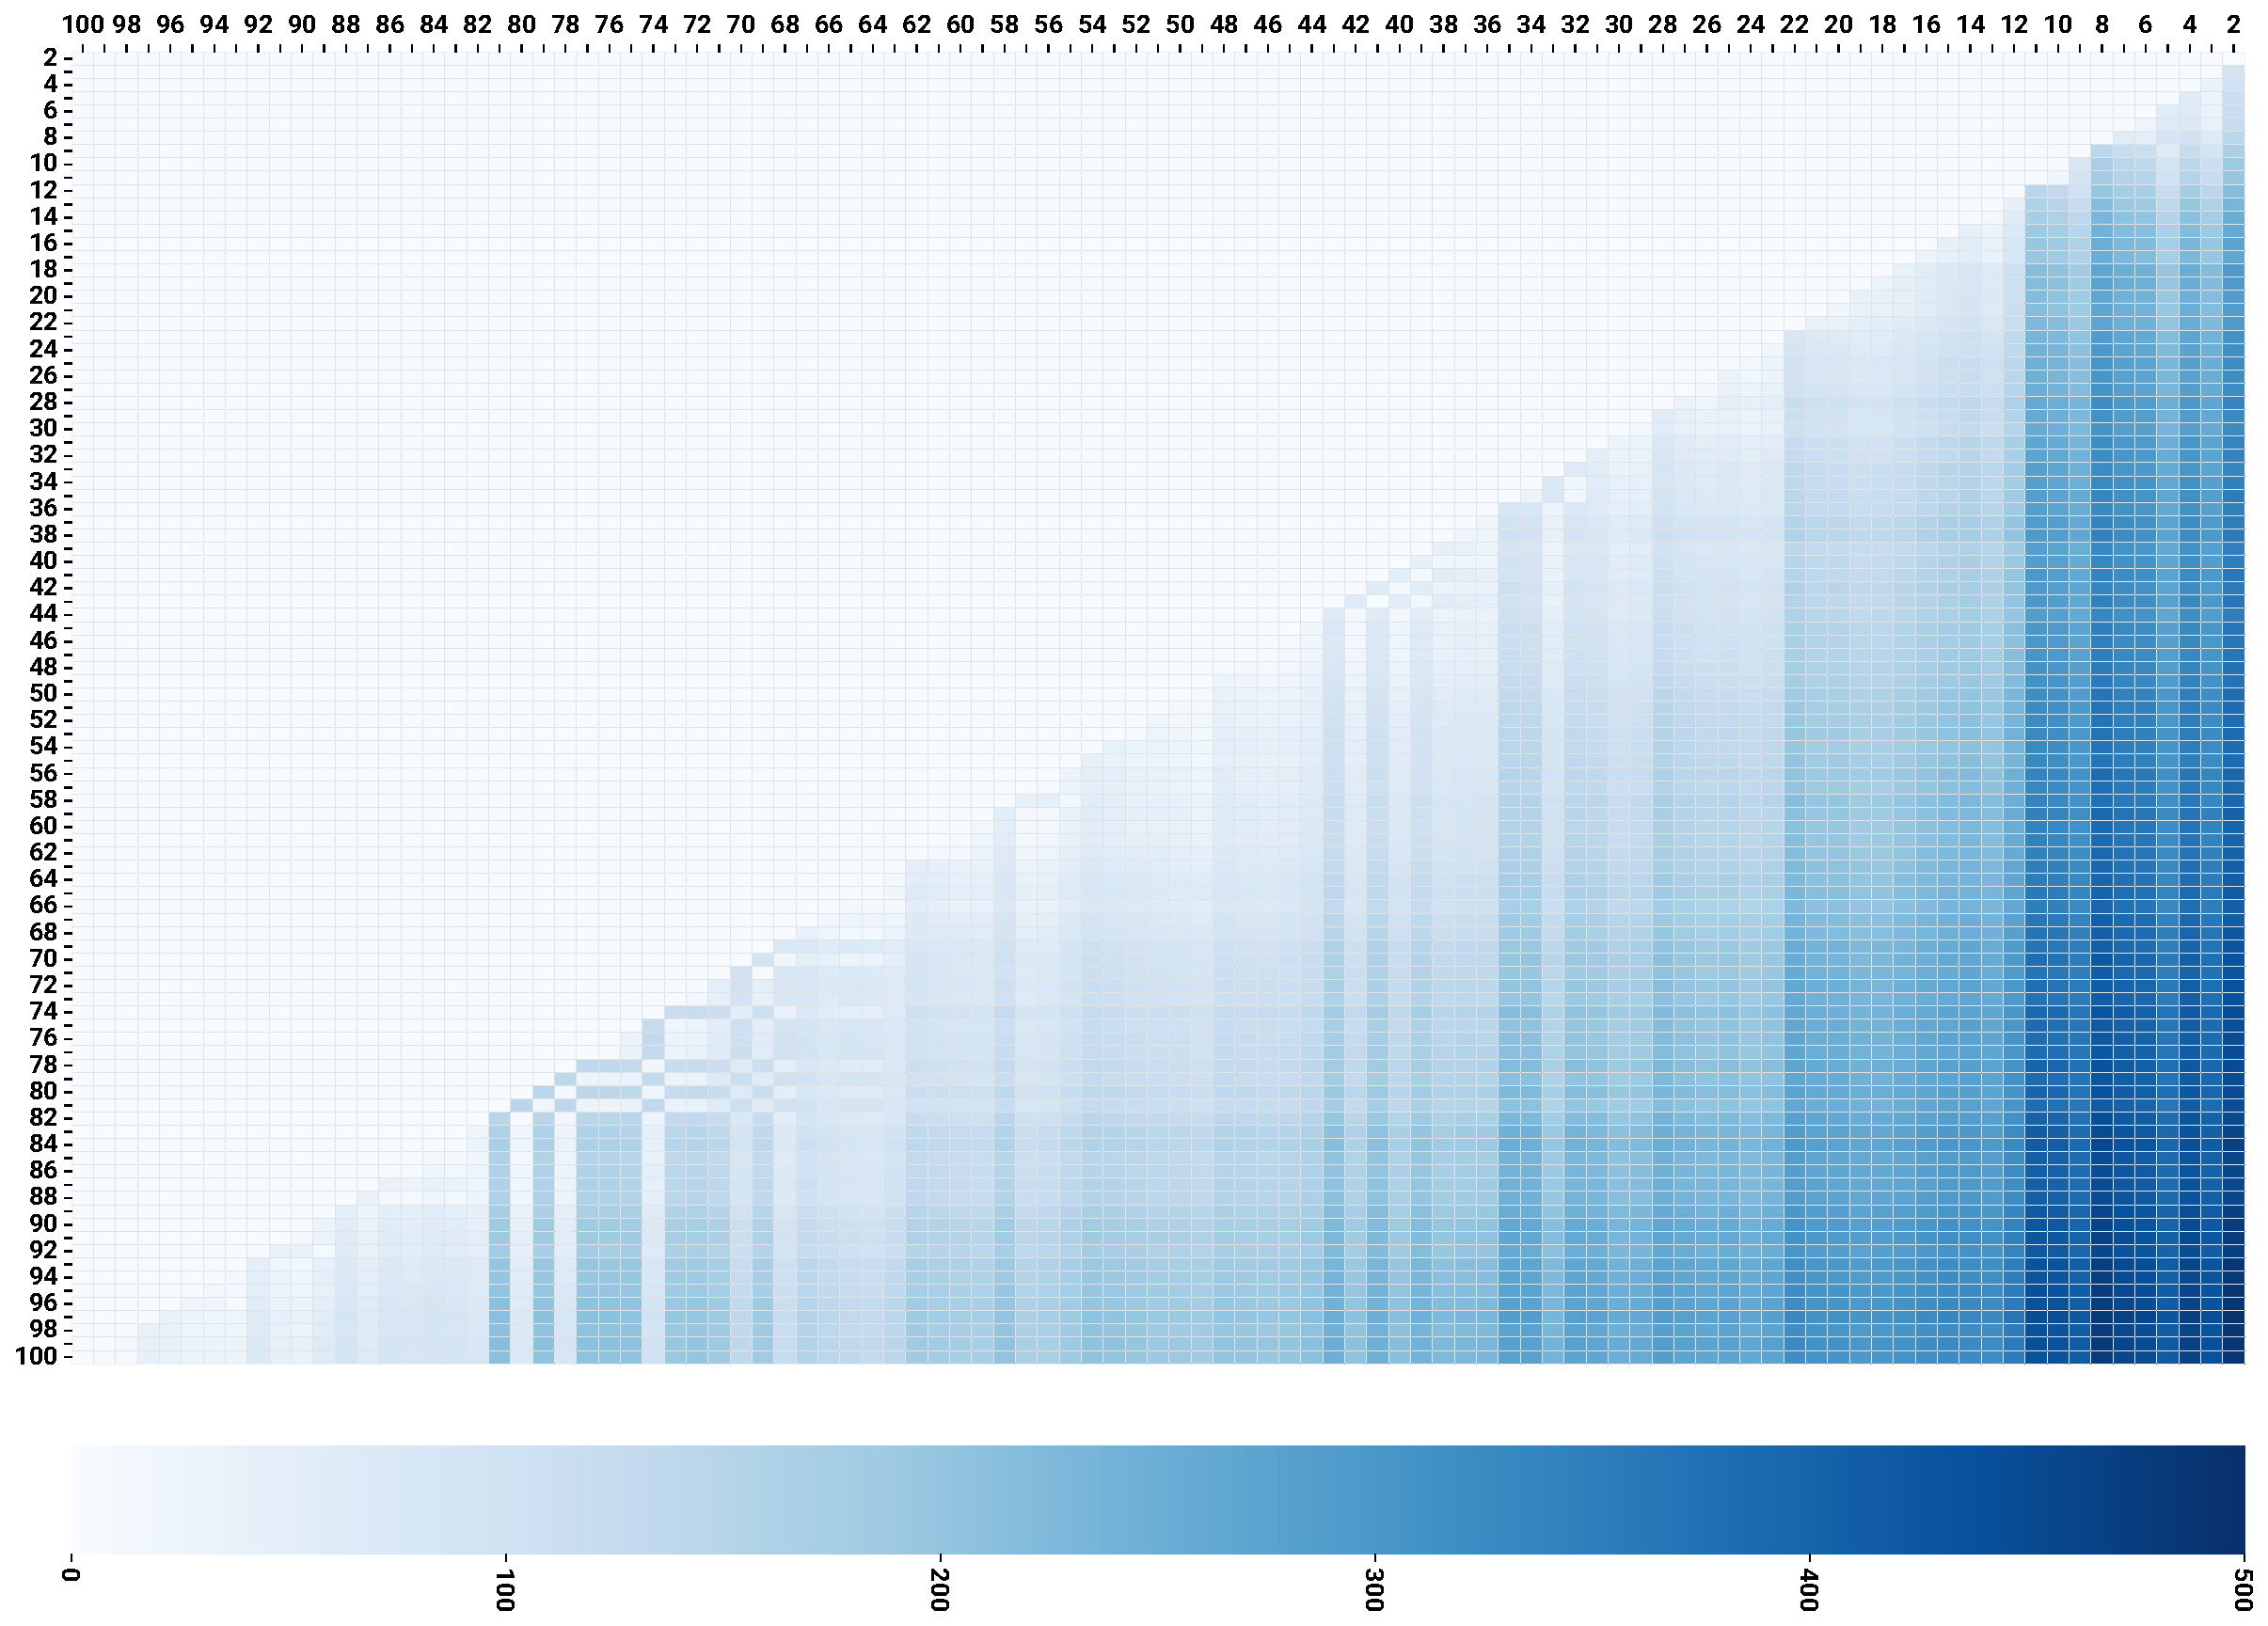
\includegraphics[width=0.8\linewidth]{{submodule/dishtiny_event_tag_phylogenetics/teeplots/distance_matrix_no_outliers/cmap=blues+linecolor=88888820+viz=heatmap+ext=}}

\caption{
TODO
}
\label{fig:phylo_distance_matrix_heatmap}
\end{figure*}



\begin{figure*}
\centering
\includegraphics[width=0.8\linewidth]{{submodule/dishtiny_event_tag_phylogenetics/teeplots/phylo_tree_no_outliers/viz=draw+ext=}}

\caption{
TODO
}
\label{fig:phylo_nj_tree}
\end{figure*}

\begin{figure*}
\centering
\includegraphics[width=0.8\linewidth]{{submodule/dishtiny_event_tag_phylogenetics/teeplots/scipy_linkage_tree_no_outliers/viz=draw+ext=}}

\caption{
Phylogeny of sampled focal strain representatives across stints reconstructed using hierarchical clustering algorithm \citep{virtanen2020scipy}.
Each leaf node corresponds to a sampled representative.
Representatives from stints 0 and 1, which share no common ancestry with representatives from other stints, are excluded.
Numbers refer to stint that each representative was sampled from.
Color coding and parentheticals of stint labels correspond to qualitative morph codes described in Table \ref{tab:morph_descriptions}.
}
\label{fig:phylo_scipy_linkage_tree}
\end{figure*}



\begin{figure}

% \begin{subfigure}{0.5\textwidth}

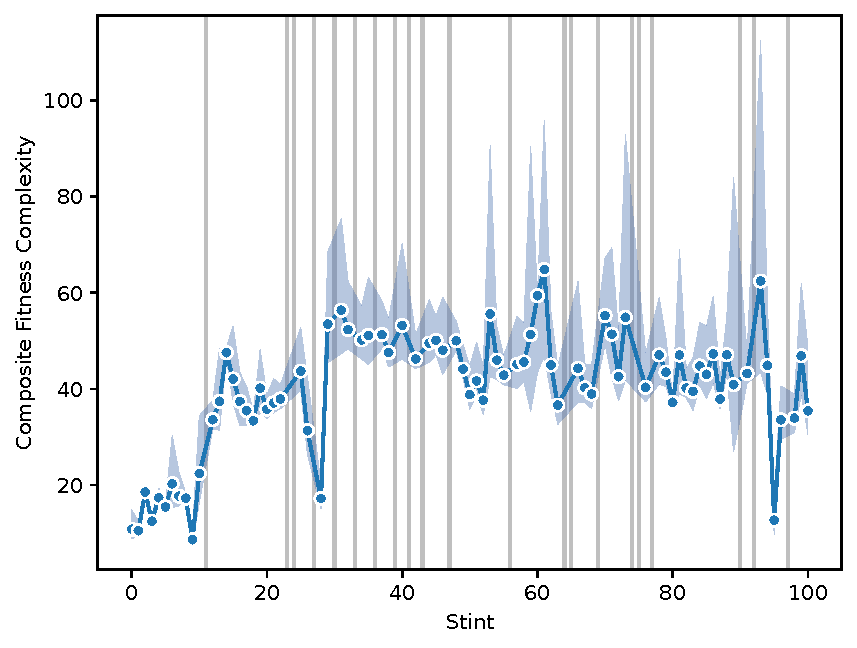
\includegraphics[width=\linewidth]{{plots/composite_fitness_complexity_alt/bucket=prq49+ci=95+endeavor=16+transform=filter-Series-16005+viz=scatter-err-vline+x=stint+y=composite-fitness-complexity+ext=}}

\caption{ Composite fitness complexity.
% An alternate rendering of Figure \ref{fig:fitness_complexity:composite_fitness_complexity}.
}
\label{fig:fitness_complexity_alt:composite_fitness_complexity_alt}

\end{subfigure}%

% \begin{subfigure}{0.5\textwidth}

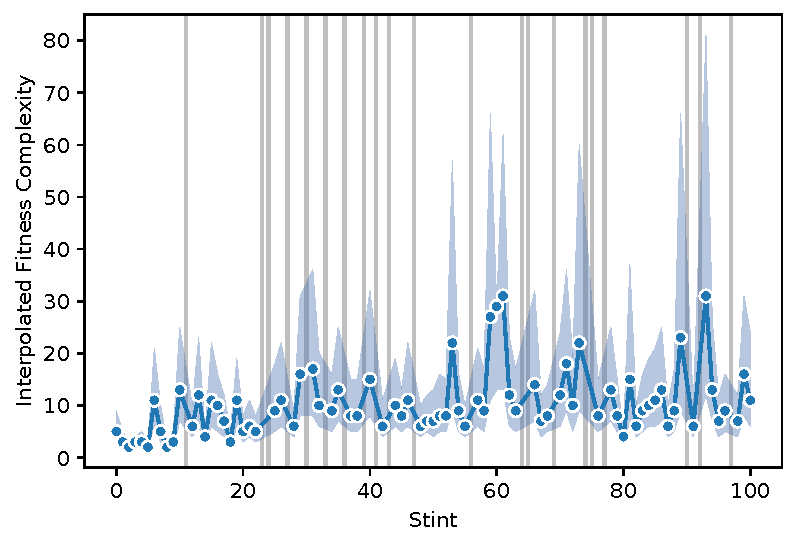
\includegraphics[width=\linewidth]{{plots/interpolated_fitness_complexity_alt/bucket=prq49+endeavor=16+transform=filter-Series-16005+viz=scatter-err-vline+x=stint+y=interpolated-fitness-complexity+ext=}}

\caption{ Interpolated fitness complexity. 
% An alternate rendering of Figure \ref{fig:fitness_complexity:interpolated_fitness_complexity}.
}
\label{fig:fitness_complexity_alt:interpolated_fitness_complexity_alt}

\end{subfigure}%

\caption{
Stub of content removed from supplement.
Left in to maintain figure numbering.
% Alternate renderings of Figure \ref{fig:fitness_complexity}.
}
\label{fig:fitness_complexity_alt}

\end{figure}


\begin{figure*}

\begin{subfigure}{0.5\textwidth}

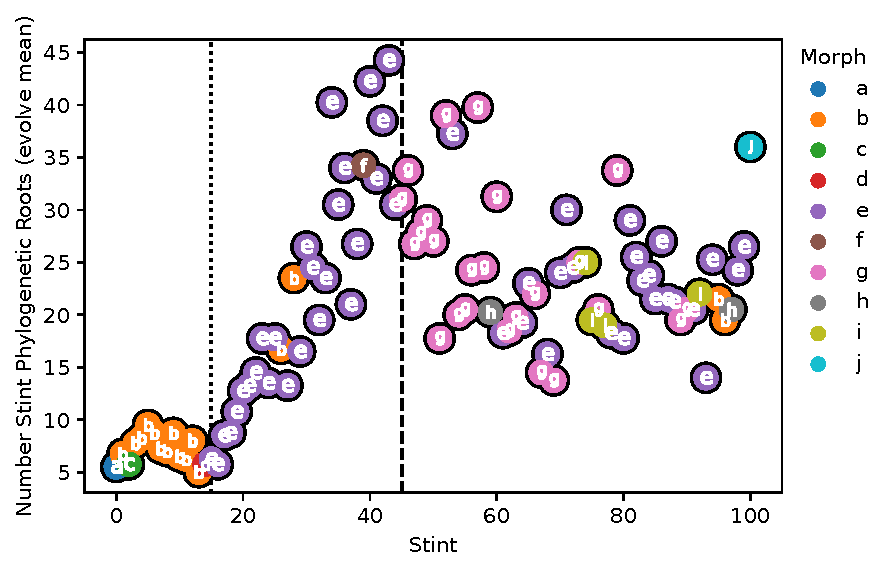
\includegraphics[width=\linewidth]{{plots/phylogeny/bucket=prq49+cat=morph+endeavor=16+transform=filter-Series-16005+viz=letterscatter-vline+x=stint+y=number-stint-phylogenetic-roots-evolve-mean+ext=}}

\caption{
Number of genomes from the beginning of a stint with extant offspring at the end of that stint. 
}
\label{fig:phylogeny:stint_roots}

\end{subfigure}%
\begin{subfigure}{0.5\textwidth}

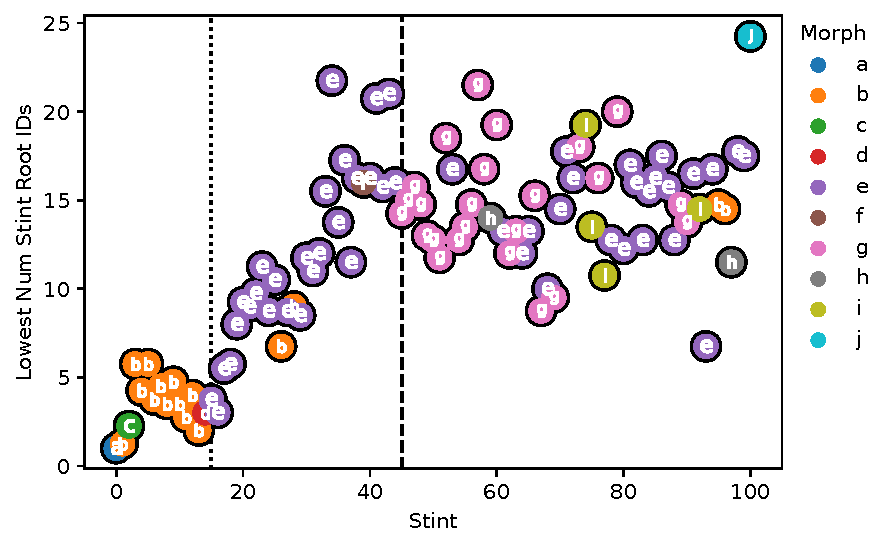
\includegraphics[width=\linewidth]{{plots/phylogeny/bucket=prq49+cat=morph+endeavor=16+transform=filter-Series-16005+viz=letterscatter-vline+x=stint+y=lowest-num-stint-root-ids+ext=}}

\caption{ Number of genomes with the lowest surviving original phylogenetic root ID from the beginning of a stint with extant offspring at the end of that stint.  }
\label{fig:phylogeny:lowestroot_stint_roots}

\end{subfigure}%
\begin{subfigure}{0.5\textwidth}

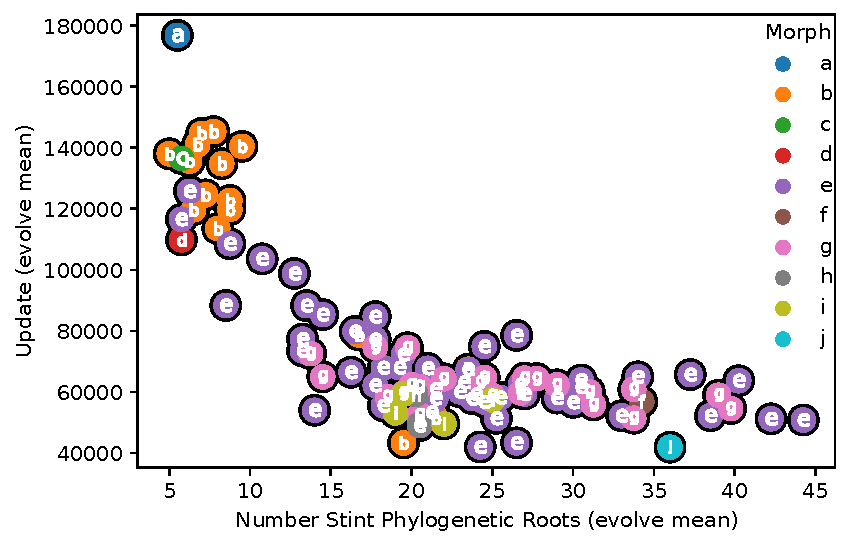
\includegraphics[width=\linewidth]{{plots/simulation/bucket=prq49+cat=morph+endeavor=16+transform=filter-Series-16005+viz=letterscatter+x=number-stint-phylogenetic-roots-evolve-mean+y=update-evolve-mean+ext=}}

\caption{
Relationship between number of simulation updates elapsed in a stint and the number of genomes seeded into a stint with extant descendants at the end of that stint.
}
\label{fig:phylogeny:updates_vs_stint_roots}

\end{subfigure}%

\begin{subfigure}{0.5\textwidth}

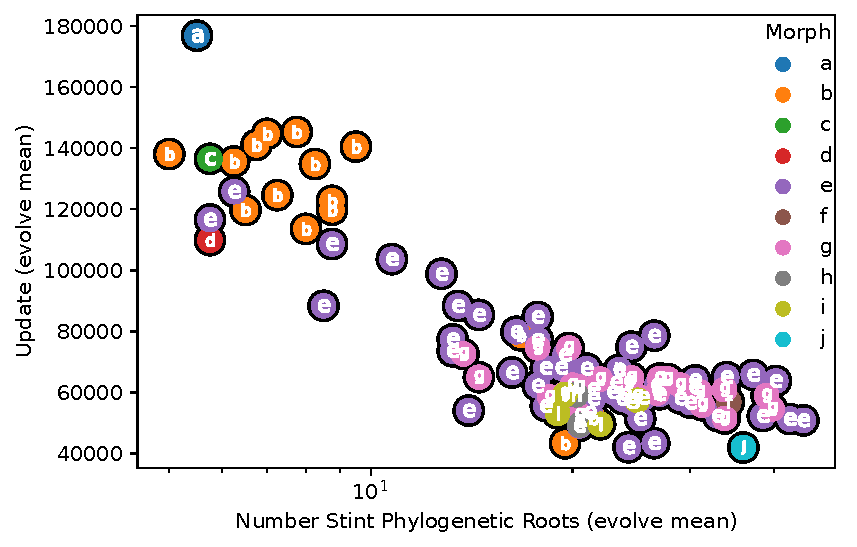
\includegraphics[width=\linewidth]{{plots/simulation/bucket=prq49+cat=morph+endeavor=16+transform=filter-Series-16005+viz=log-letterscatter+x=number-stint-phylogenetic-roots-evolve-mean+y=update-evolve-mean+ext=}}

\caption{ Relationship between number of simulation updates elapsed in a stint and the number of genomes seeded into a stint with extant descendants at the end of that stint, log axis. }
\label{fig:phylogeny:log_updates_vs_stint_roots}

\end{subfigure}%


\caption{
Phylogenetic statistics.
Color coding and letters correspond to qualitative morph codes described in Table \ref{tab:morph_descriptions}.
Dotted vertical line denotes emergence of morph $e$.
Dashed vertical line denotes emergence of morph $g$.
}
\label{fig:phylogeny}
\end{figure*}


\begin{figure*}

\begin{subfigure}{0.5\textwidth}

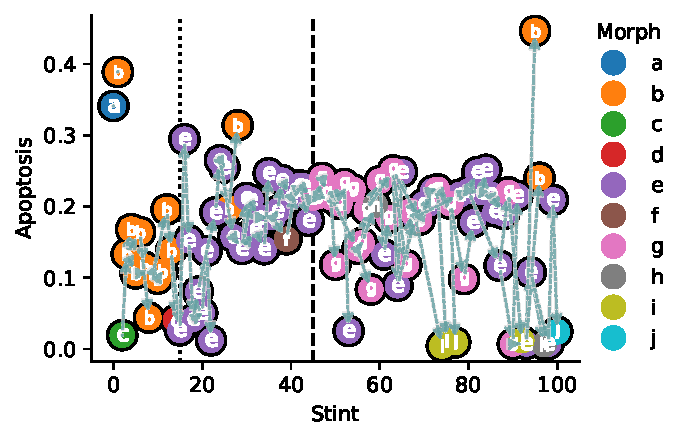
\includegraphics[width=\linewidth]{{plots/apoptosis_stint/bucket=prq49+cat=morph+endeavor=16+transform=filter-Series-16005+viz=letterscatter-vline+x=stint+y=fraction-deaths-apoptosis-monoculture-mean+ext=}}

\caption{Fraction of cell deaths due to apoptosis.
Color coding and letters correspond to qualitative morph codes described in Table \ref{tab:morph_descriptions}.}
\label{fig:apoptosis:apoptosis_stint}

\end{subfigure}%

\begin{subfigure}{0.5\textwidth}

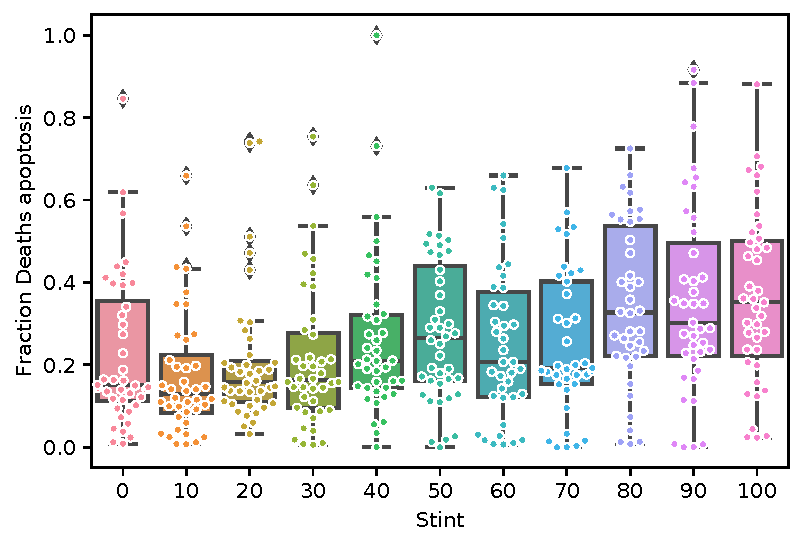
\includegraphics[width=\linewidth]{{plots/apoptosis_distn/bucket=prq49+endeavor=16+transform=filter-Stint-mod10+viz=swarmplot-boxplot+x=stint+y=fraction-deaths-apoptosis+ext=}}

\caption{Distribution of apoptosis rates across evolutionary replicates.}
\label{fig:apoptosis:apoptosis_distn}

\end{subfigure}%


\caption{ Apoptosis rates in case study strain and across evolutionary replicates. }
\label{fig:apoptosis}
\end{figure*}

\begin{figure}

\begin{subfigure}{0.5\textwidth}

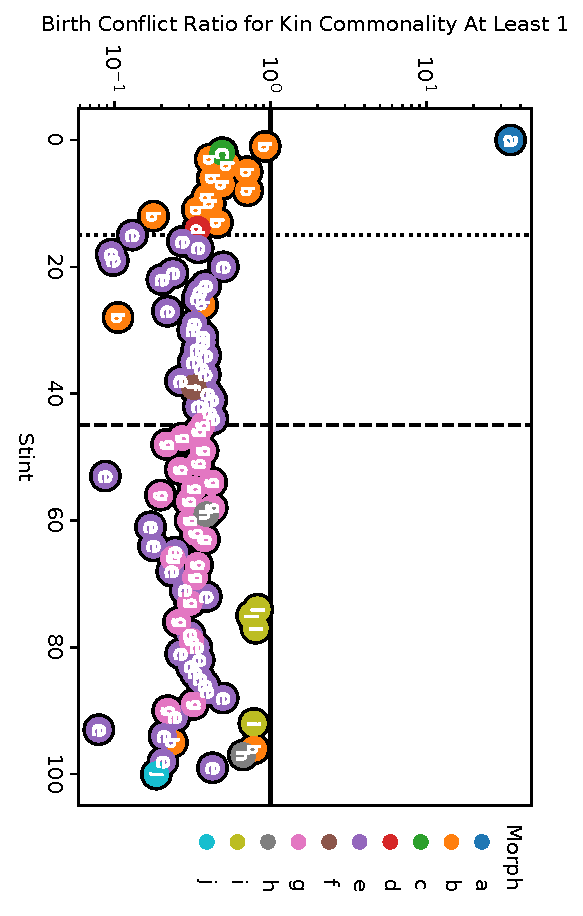
\includegraphics[width=\linewidth]{{plots/conflict/at_least_one/bucket=prq49+cat=morph+endeavor=16+transform=filter-Series-16005+viz=log-letterscatter-vline-hline+x=stint+y=birth-conflict-ratio-for-kin-commonality-at-least-1+ext=}}

\caption{
Frequency at which cell proliferation replaces neighbors with any kin group commonality to the parent, normalized for the relative frequency of neighbors with kin group commonality to the parent.
Values below 1.0 (horizontal bar) indicate preference to displace neighbors with no kin group commonality.
}
\label{fig:conflict:at_least_one}

\end{subfigure}%
\begin{subfigure}{0.5\textwidth}

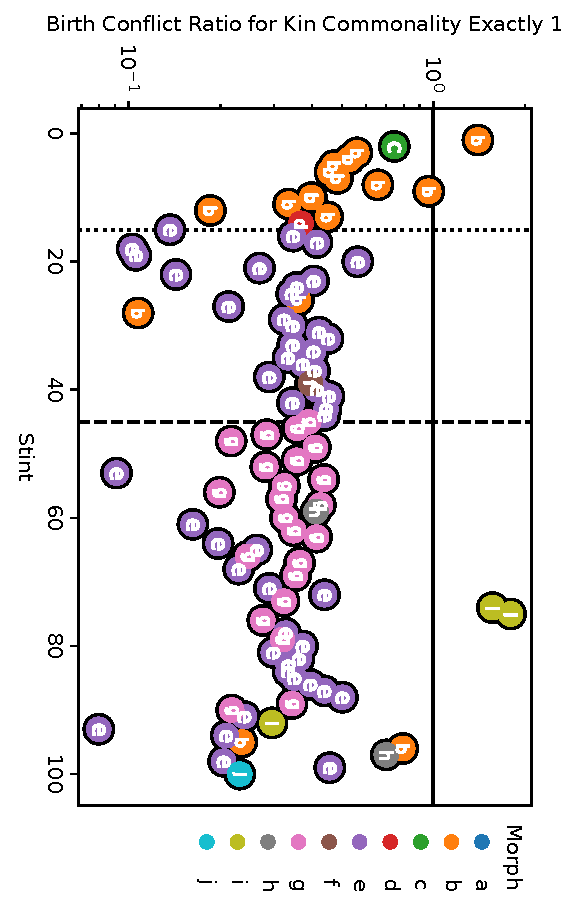
\includegraphics[width=\linewidth]{{plots/conflict/exactly_one/bucket=prq49+cat=morph+endeavor=16+transform=filter-Series-16005+viz=log-letterscatter-vline-hline+x=stint+y=birth-conflict-ratio-for-kin-commonality-exactly-1+ext=}}

\caption{
Frequency at which cell proliferation replaces neighbors with only outer kin group commonality to the parent, normalized for the relative frequency of neighbors with kin group commonality to the parent.
Values below 1.0 (horizontal bar) indicate preference to displace neighbors with no kin group commonality.
}
\label{fig:conflict:exactly_one}

\end{subfigure}%

\begin{subfigure}{0.5\textwidth}

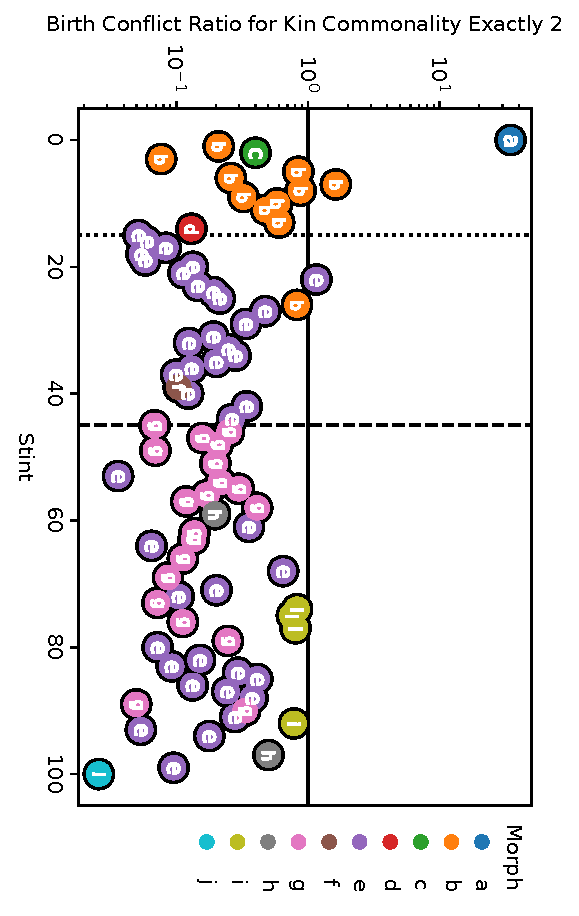
\includegraphics[width=\linewidth]{{plots/conflict/exactly_two/bucket=prq49+cat=morph+endeavor=16+transform=filter-Series-16005+viz=log-letterscatter-vline-hline+x=stint+y=birth-conflict-ratio-for-kin-commonality-exactly-2+ext=}}

\caption{
Frequency at which cell proliferation replaces neighbors with full kin group commonality to the parent, normalized for the relative frequency of neighbors with kin group commonality to the parent.
Values below 1.0 (horizontal bar) indicate preference to displace neighbors without full kin group commonality.
}
\label{fig:conflict:exactly_two}

\end{subfigure}%


\caption{ Kin conflict rates.
Color coding and letters correspond to qualitative morph codes described in Table \ref{tab:morph_descriptions}.}
\label{fig:conflict}

\end{figure}
\begin{figure*}

\begin{subfigure}{0.5\textwidth}

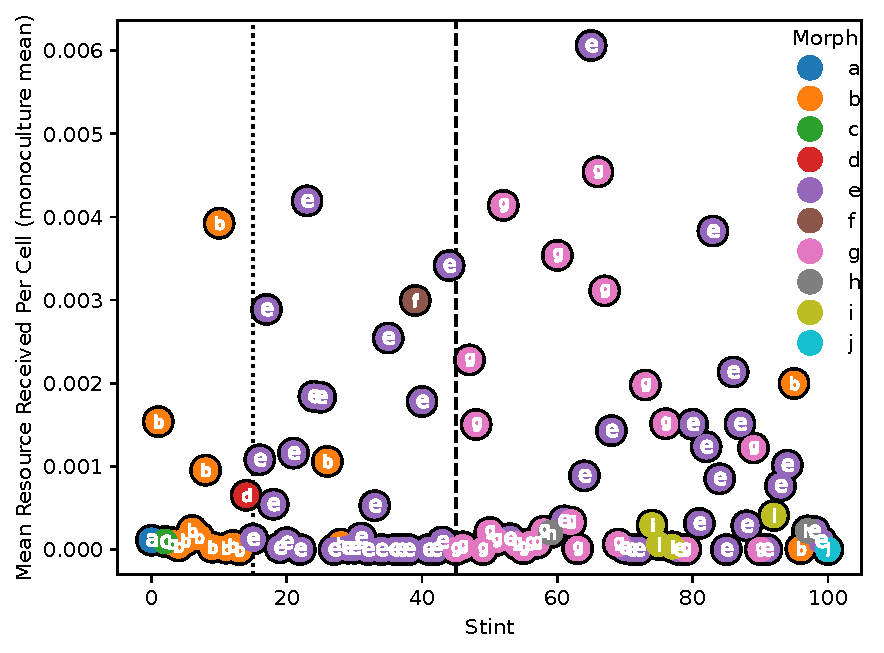
\includegraphics[width=\linewidth]{{plots/resource_sharing/bucket=prq49+cat=morph+endeavor=16+transform=filter-Series-16005+viz=letterscatter-vline+x=stint+y=mean-resource-received-per-cell-monoculture-mean+ext=}}

\caption{ Fraction of cells receiving shared resource at end of evolutionary stints, including not just the focal lineage. }
\label{fig:resource_sharing:fraction_sharing_evolve}

\end{subfigure}%

\begin{subfigure}{0.5\textwidth}

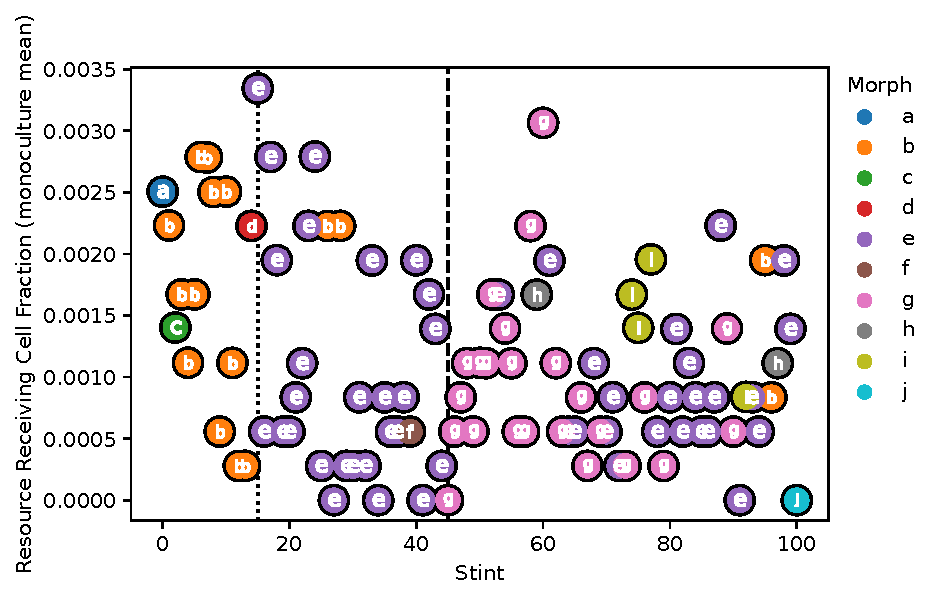
\includegraphics[width=\linewidth]{{plots/resource_sharing/bucket=prq49+cat=morph+endeavor=16+transform=filter-Series-16005+viz=letterscatter-vline+x=stint+y=resource-receiving-cell-fraction-monoculture-mean+ext=}}

\caption{ Fraction of cells receiving shared resource in monocultures of focal lineage. }
\label{fig:resource_sharing:fraction_sharing_monoculture}

\end{subfigure}%

\begin{subfigure}{0.5\textwidth}

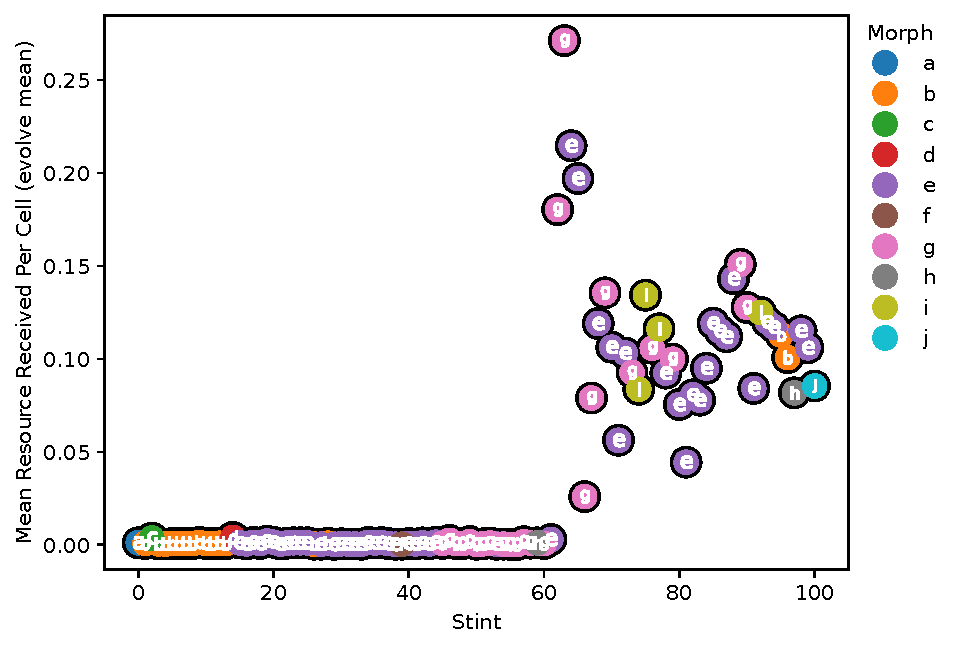
\includegraphics[width=\linewidth]{{plots/resource_sharing/bucket=prq49+cat=morph+endeavor=16+transform=filter-Series-16005+viz=letterscatter+x=stint+y=mean-resource-received-per-cell-evolve-mean+ext=}}

\caption{ Mean amount of resource shared per cell-update at end of evolutionary stints, including not just the focal lineage. }
\label{fig:resource_sharing:sharing_amount_evolve}

\end{subfigure}%
\begin{subfigure}{0.5\textwidth}

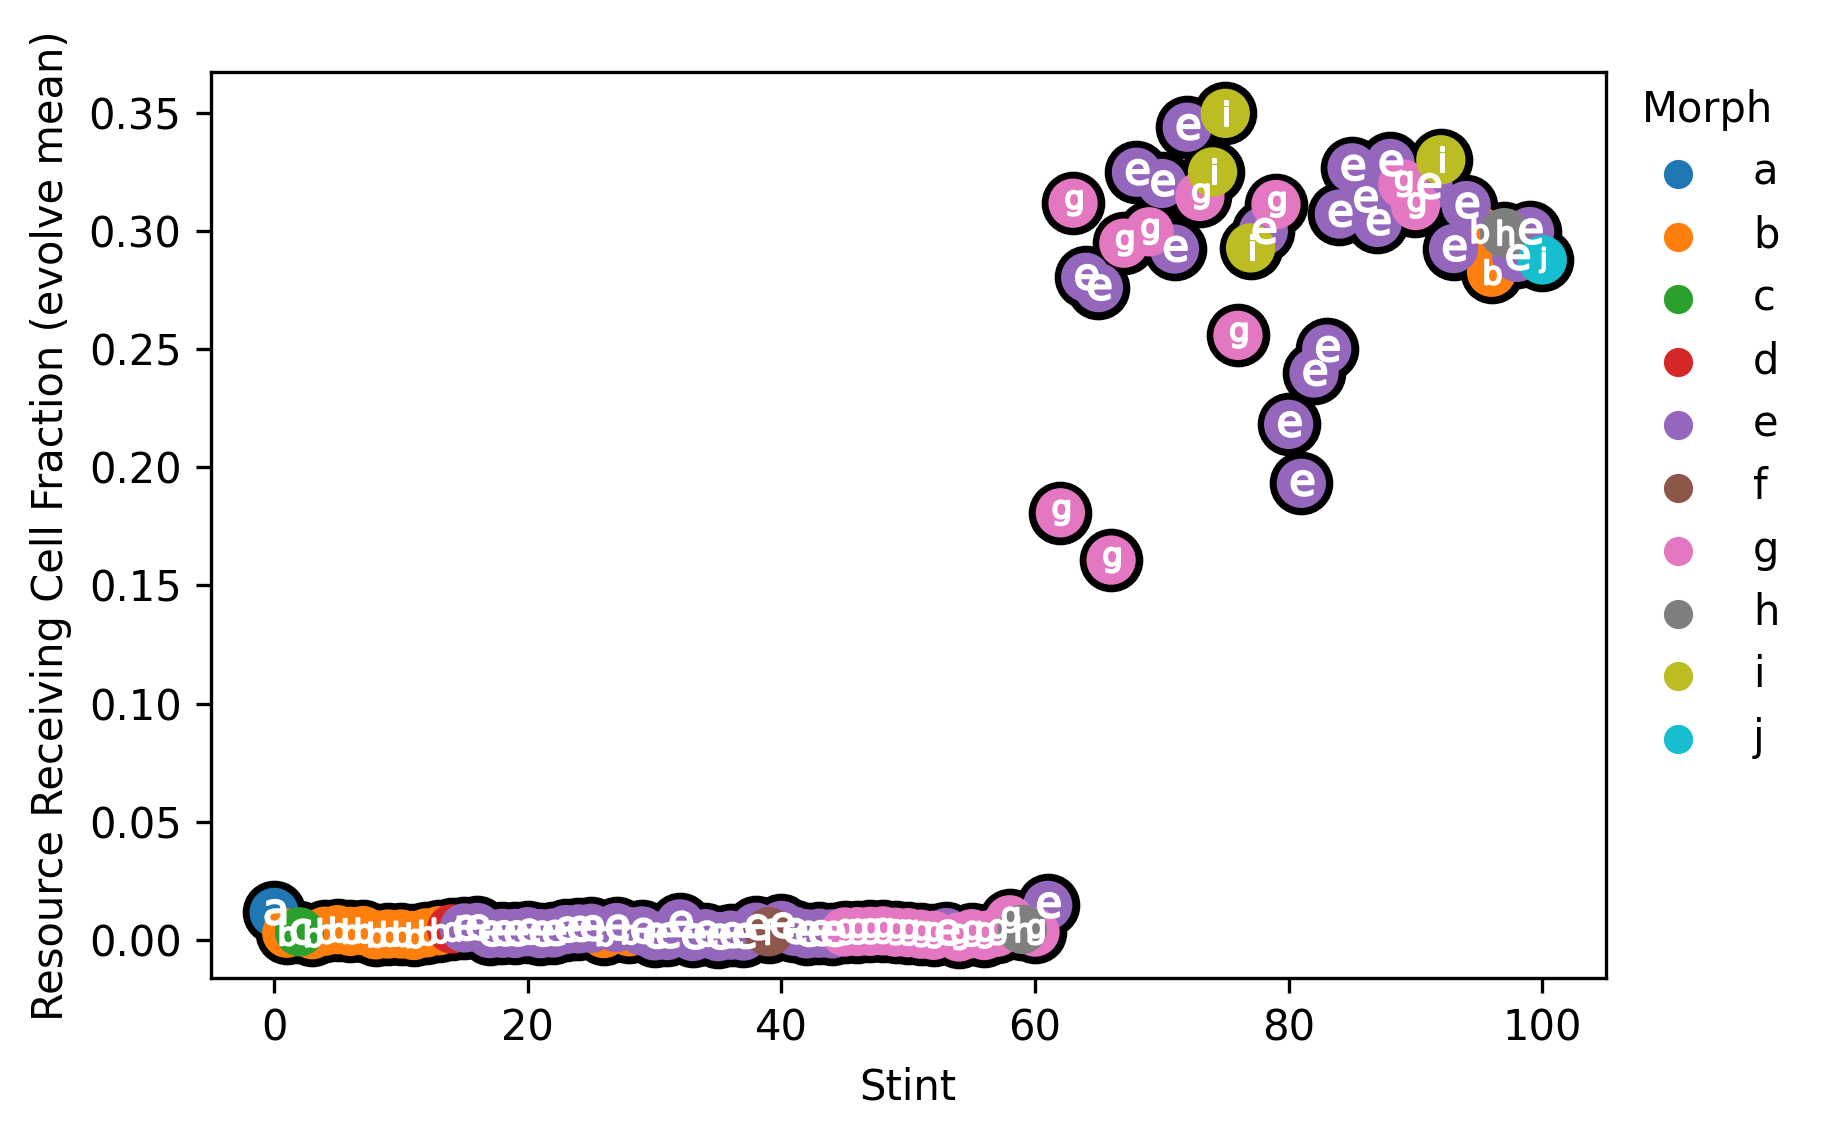
\includegraphics[width=\linewidth]{{plots/resource_sharing/bucket=prq49+cat=morph+endeavor=16+transform=filter-Series-16005+viz=letterscatter+x=stint+y=resource-receiving-cell-fraction-evolve-mean+ext=}}

\caption{Mean amount of resource shared per cell-update in monocultures of focal lineage. }
\label{fig:resource_sharing:sharing_amount_monoculture}

\end{subfigure}%


\caption{
\textbf{Resource-sharing phenotypic traits.}
\footnotesize
Color coding and letters correspond to qualitative morph codes described in Table \ref{tab:morph_descriptions}.
Dotted vertical line denotes emergence of morph $e$.
Dashed vertical line denotes emergence of morph $g$.
}
\label{fig:resource_sharing}
\end{figure*}

\begin{figure*}

\begin{subfigure}{0.5\textwidth}

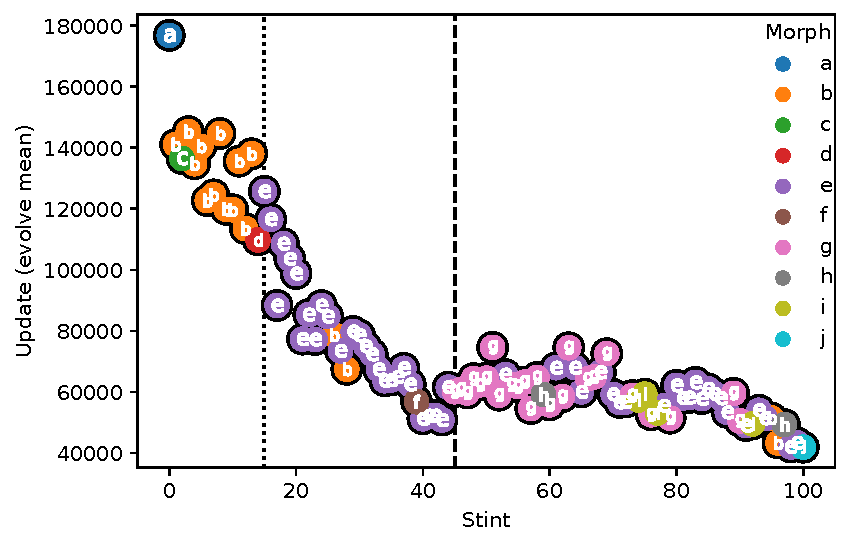
\includegraphics[width=\linewidth]{{plots/simulation/bucket=prq49+cat=morph+endeavor=16+transform=filter-Series-16005+viz=letterscatter-vline+x=stint+y=update-evolve-mean+ext=}}

\caption{ Number simulation updates elapsed per three-hour evolutionary stint. Color coding and letters correspond to qualitative morph codes described in Table \ref{tab:morph_descriptions}. }
\label{fig:simulation:stint_updates}

\end{subfigure}%

\begin{subfigure}{0.5\textwidth}

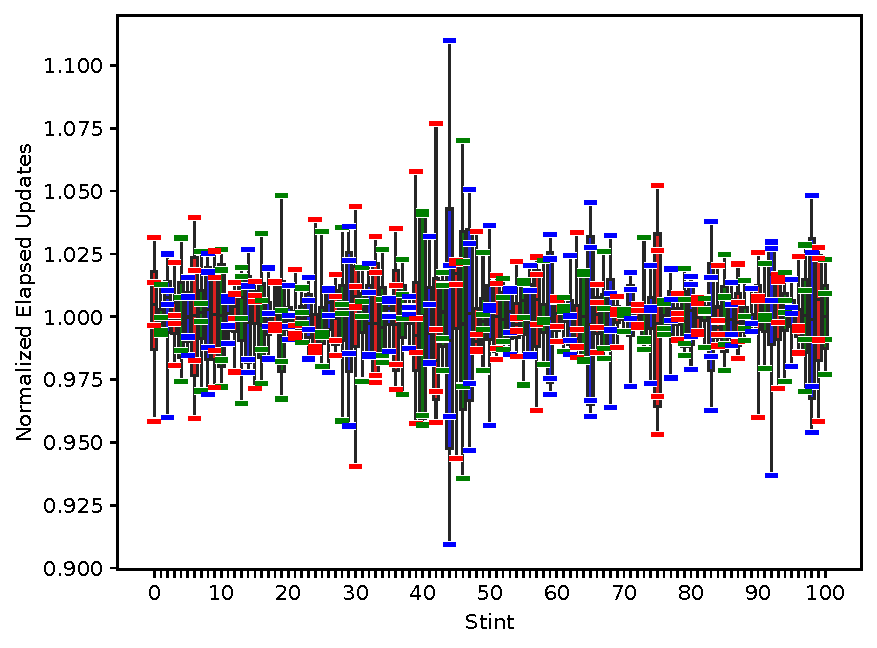
\includegraphics[width=\linewidth]{{plots/simulation/bucket=prq49+endeavor=16+hue=stint+transform=filter-Series-16005+viz=boxstrip+x=stint+y=normalized-elapsed-updates+ext=}}

\caption{ Distribution of real-time simulation rate of concurrent threads. Colors provided only to distinguish neighboring data. }
\label{fig:simulation:thread_updates}

\end{subfigure}%

\caption{ Real-time simulation performance. }
\label{fig:simulation}
\end{figure*}



\end{document}
